\documentclass[mscthesis]{usiinfthesis}
\usepackage{lipsum}
\usepackage{mathtools}
\usepackage{listings}
\usepackage{subcaption}
\usepackage[most]{tcolorbox}
\usepackage{xcolor,pifont}
\usepackage{color} % for the command \textcolor
\usepackage{soul} % for the command \hl
\newboolean{showcomments}
\setboolean{showcomments}{true}
\ifthenelse{\boolean{showcomments}}
{\newcommand{\nb}[2] {
		\fcolorbox{black}{gray!20}{\bfseries\sffamily\scriptsize#1:}
		{\sf\small$\blacktriangleright$\textit{#2}$\blacktriangleleft$}
	}
}
{\newcommand{\nb}[2]{}
}
\newcommand\matteo[1]{\nb{Matteo}{\hl{#1}}}
\lstset
{
    language=Python,
    breaklines=true,
    basicstyle=\footnotesize,
    frame=single,
    numbers=left,
    stepnumber=1,
    tabsize=1,
    frameround=fttt
}
\usepackage{graphicx}
\usepackage{wrapfig}
\usepackage{multirow}
\graphicspath{{images/}}

\lstdefinelanguage{algebra}
{morekeywords={import,sort,constructors,observers,transformers,axioms,if,
else,end},
sensitive=false,
morecomment=[l]{//s},
}

\title{Reinforcement learning vs supervised learning} %compulsory
\specialization{Major in Artificial intelligence}%optional
\subtitle{A comparison on DonkeyCar autonomous driving} %optional 
\author{Giorgio Macauda} %compulsory
\begin{committee}
\advisor{Prof.}{Paolo}{Tonella} %compulsory
\coadvisor{PhD}{Matteo}{Biagiola}{} %optional
\end{committee}
\Day{12} %compulsory
\Month{September} %compulsory
\Year{2022} %compulsory, put only the year
\place{Lugano} %compulsory

\dedication{To my beloved} %optional
\openepigraph{Someone said \dots}{Someone} %optional

%\makeindex %optional, also comment out \theindex at the end

\begin{document}

\maketitle %generates the titlepage, this is FIXED

\frontmatter %generates the frontmatter, this is FIXED

\begin{abstract}
This is a very abstract abstract. 
\lipsum
\end{abstract}
\begin{acknowledgements}
\lipsum 
\end{acknowledgements}

\tableofcontents 
\listoffigures %optional
\listoftables %optional

\mainmatter

\chapter{Introduction}

Reinforcement Learning (RL) is a branch of machine learning that has proven to be a very general framework to learn sequential decision-making tasks modeled as Markov Decision Processes (MDP) \citep{vanOtterlo2012} without the need for labeled data. Under this framework, an RL agent interacts with an environment in discrete time steps, observing the state of the environment and deciding actions based on it, in order to maximize a given reward function to solve a certain task. Such task is usually \textit{episodic}, i.e., there are clear boundaries to determine when the task is achieved.

The first RL algorithms were tabular and could solve simple tasks and games~\cite{Sutton1998}. The advent of \textit{Deep Learning} made it possible for RL algorithms to scale towards interesting and challenging problems, where the state and/or the action space are too big to be stored in tables (e.g. images and continuous actions). Most notably, the first Deep RL (DRL) algorithm, called Deep Q Network, was able to surpass humans in most of the Atari games~\cite{atari}. Recent developments in RL have shown how the framework can deal with even more complex games, from the game of Go~\cite{alphago} to multiplayer games such as Starcraft II~\cite{alphastar} and Dota II~\cite{opeaifive}.

Despite the impressive performance, RL is still confined to simulated environments, where training data can be easily collected by running several instances in parallel and safety is not a primary concern. Indeed, progress towards bringing RL into the real world, has been much slower w.r.t. the progress made in simulation, given the higher complexity and unpredictability of real-world environments. One of the domains in which RL has been applied to the real world is robotics~\cite{smith2022walk,pmlr-v164-raffin22a,gu2017deep}. However, training RL agents to control physical robots in the real world presents several challenges that are absent in simulation. First of all, training cannot be easily parallelized and therefore the RL algorithm needs to be \textit{data-efficient}, i.e., it needs to be able to reuse the collected experience for training since acquiring data is costly. Secondly, the movements of the robot need to be taken into account both to protect the environment around the robot that might carry out unsafe actions during learning and to safeguard the robot itself that can be damaged by the high-frequency actions the robot is controlled with. Moreover, the number of sensors in the real world is limited compared to simulated environments. Having less sensors impacts the design of the reward function that is necessarily more \textit{sparse} (i.e. it gives less guidance to the agent during training) than in simulation. Finally, when the RL agent completes an episode, either successfully or unsuccessfully, a \textit{reset} of the environment is needed, in order to restore its initial state. Depending on the context, such task in the real world might require substantial human intervention.

Positive results in training RL agents to control robots in the real world often come from very constrained applications. For instance, the OpenAI team was able to train a RL agent to control a robotic hand in order to solve the Rubik's cube~\cite{rubik}. Other examples are robotic arms that have been trained to reach a certain object, pull or push a door and to pick an object and place it in a target location~\cite{gu2017deep}. The whole RL training process for such tasks can be almost entirely automated requiring little to no human supervision.

On the other hand, there are fewer tasks that have been addressed with RL in real-world uncontrolled environments~\cite{smith2022walk,DBLP:journals/corr/abs-2008-00715}. In this thesis we target with RL the problem of \textit{self-driving} and, in particular, we are interested in the \textit{lane-keeping} task in which the RL agent needs to control a car to drive along a predetermined track. This problem is usually tackled using the Supervised Learning (SL) approach both in academia and in industry. In such learning paradigm a dataset of driving experience is collected, usually composed of pairs of images and labels. In its simplest form the label is the recorded steering angle applied by the human driver corresponding to a certain image. Then, the dataset is used to train a Deep Neural Network (DNN) to minimize the error between the predicted steering angle and the ground truth label. Even though SL has proven successful for this task in the real world, it has some disadvantages. First, it requires huge labeled datasets that need to be constantly updated to take into account new scenarios. Furthermore, a SL model is trained offline and, as such, it cannot predict the effects that a certain action has on the environment. On the other hand, a RL agent is trained online, thereby being able to learn and adapt based on the effects of its actions, respecting the sequential nature of the task of driving.

%Interesting results in real-world applications comes often from very controlled environments, for example, solving a Rubik's cube requires a limited set of actions, and the reset of the cube to the initial state is very simple. The objective of this thesis is to learn an RL self-driving DonkeyCar, a scale remote-controlled electric car, first in simulation and then replicate the same result in a very uncontrolled real-world environment. The state-of-the-art self-driving cars algorithms, created by Google with Waymo and Tesla, rely on Supervised Learning (SL) techniques such as Convolutional Neural Networks (CNNs) for image processing, feature detection, and extraction, and Recurrent Neural Networks (RNNs) for processing temporal data. Even though supervised learning is very successful in autonomous driving, it does not come at no cost, it requires huge labeled datasets that need to be consistently updated to face new scenarios. Furthermore, SL methods typically are used to generate predictions about the surroundings of the car and upon that decisions are taken and do not take into account that each decision influences future events, which in turn influence future decisions. In other words, they try to imitate data but do not have the consciousness of the real world. RL, on the other hand, allows learning a policy, thereby creating models able to make their own decisions, take actions, react and adapt based on the feedback they receive. 

The objective of this thesis is to train a RL agent to control a physical 1:16 scale radio-controlled car (called DonkeyCar~\footnote{https://www.donkeycar.com/}) and make it drive along a physical track. The car is equipped with a camera, which is the only sensor the agent has to perceive its surroundings. We first addressed the problem in simulation, by using a high-fidelity simulator and a faithful representation of the physical track. We use simulation to carry out experiments to evaluate different training configurations in order to select the best choice when training in the real world. In particular, we experimented with different Representation Learning (ReL) techniques to speed up learning, as learning directly from raw images is known to be ineffective~\cite{DBLP:journals/corr/abs-2008-00715}. Moreover, we evaluated different reward functions and several reset strategies. Then, we transferred this knowledge to the real world and trained a RL agent which is able to learn to drive along the physical track in a reasonable amount of time.

%Since training an autonomous agent from raw images is expensive and has been proven unsuccessful \citep{DBLP:journals/corr/abs-2008-00715}, we first investigate a few Representation Learning (ReL) techniques such as AutoEncoders and Variational AutoEncoders. ReL is a technique designed to extract abstract features from data and reduce their complexity. Furthermore, techniques for a smooth exploration of the environment such as state-dependent exploration are implemented. A reward function that has proven to work in both simulated and real-world environments has been designed even if the sensors are scarce. In particular, as a first step of the experiments, we trained successfully a simulated proof-of-work RL agent that autonomously drives by taking actions based on what a camera sensor, with which it is equipped, sees as unique information about the surroundings. As a second step, the model is successfully replicated in a real-world environment with an investigation of the best training strategy in terms of the starting point of the car which crucially defines the learning success. 

Finally, we also experimented with \textit{sim2real} (simulation to real) techniques that can be used to transfer knowledge from one environment (e.g. in simulation) to another one (e.g. in the real world). Our attempts can be useful to understand the direction of future endeavors at addressing the same problem.

%Finally, a few unsuccessful experiments which need to be explored more are run in a Sim2Real procedure through the use of CycleGan \citep{CycleGAN2017}, where an agent trained in simulation is deployed in the real world and vice-versa, thus leading to cheaper training processes and more reliable benchmarking. 

\chapter{Background}

\section{Reinforcement Learning}

Reinforcement Learning (RL) is a branch of machine learning, alongside supervised learning and unsupervised learning, that defines a set of algorithms meant to learn how to act in a specific environment without the need of labeled data to learn from. 

The algorithm defines the agent that learns a given task, for example, walking, driving and playing a game, by trial and error, while interacting with an environment which can be real or simulated. Whenever the agent makes a set of good actions it receives a positive reward, which makes such actions more likely in the future. State, action and reward are the most important concepts in RL. The state represents the current situation of the environment. If the agent is a humanoid robot and the task is walking, one possible state representation is the positions of its actuated joints. The action set or space in case of continuous domain, describes what the agent can do in a particular state. In the humanoid robot example above, the action space is a n-dimensional vector where each dimension represents the torque command to each of the n joint motors. Finally the reward is a measure of how good are the actions carried out by the agent. 

\begin{wrapfigure}{r}{0.6\textwidth}
  \begin{center}
    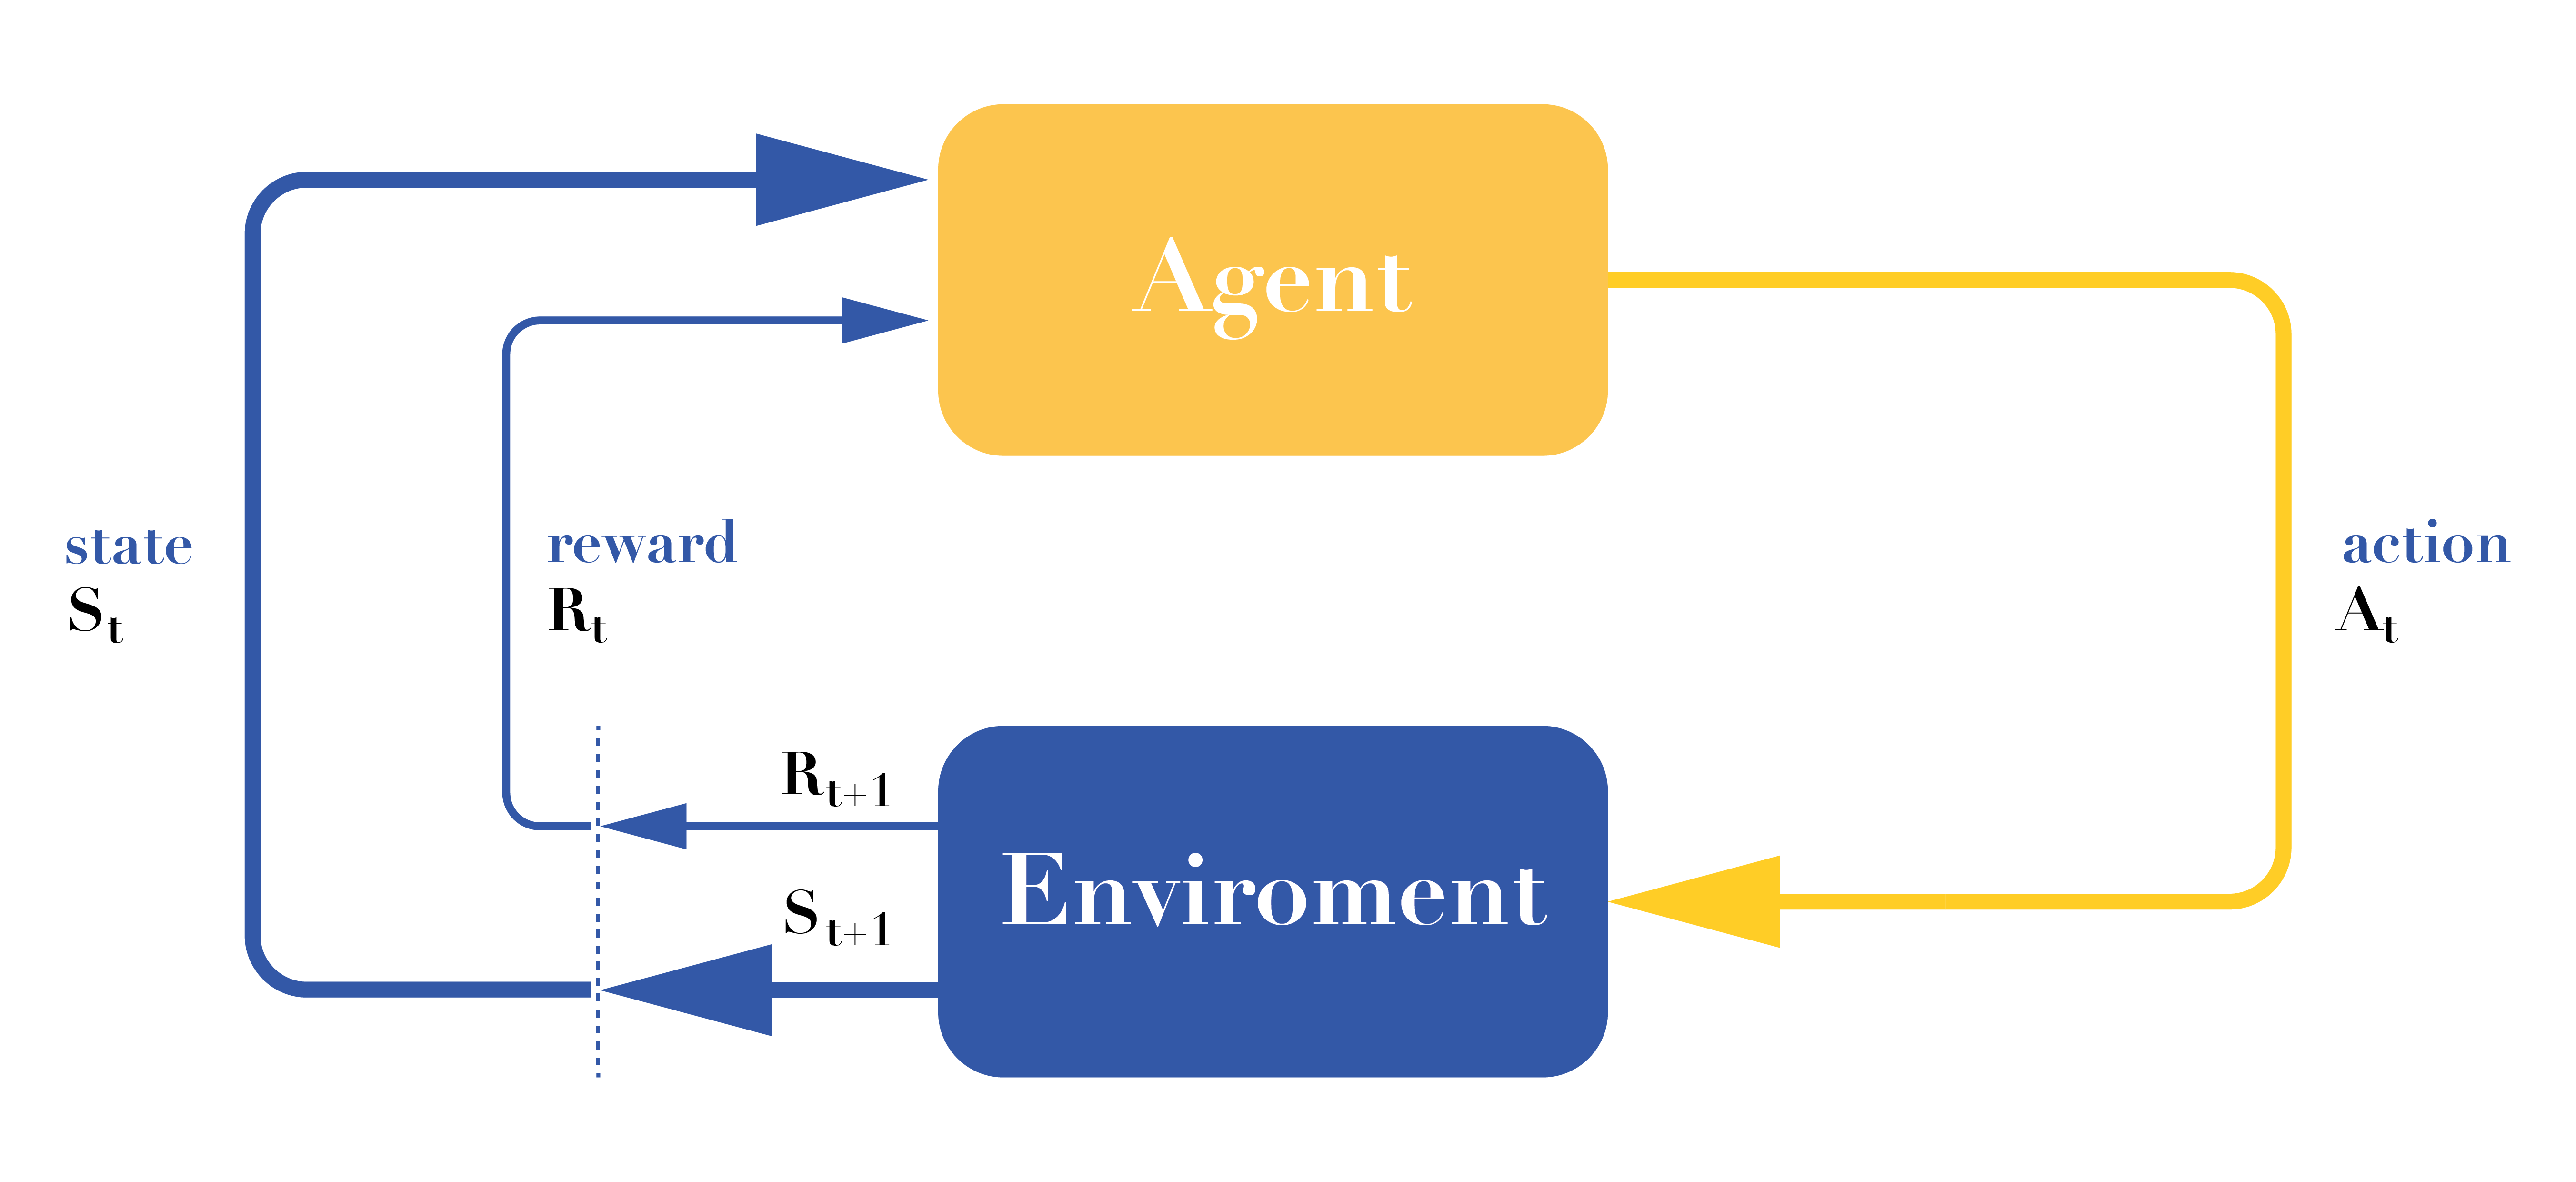
\includegraphics[width=0.6\textwidth]{background/rl.png}
  \end{center}
  \caption{Basic reinforcement learning}
  \label{fig:rl}
\end{wrapfigure}

The reward function, usually human-designed, assigns a score to the action taken by the agent. Every action that leads to a \textit{good} state increases the score and vice-versa. As described in Figure \ref{fig:rl} the agent interacts with the environment in discrete time steps. At time $t$ it gets the current state $s_{t}$ and the associated reward $r_{t}$ then the action $a_{t}$ is chosen from the set of available actions. After receiving the chosen action, the environment moves to a new state $s_{t+1}$ and the reward $r_{t+1}$ is given back to the agent. The total discounted reward (also known as return) to be maximized is:

\begin{equation}
  \label{eq:totalreward}
  R=\sum _{t=0}^{T}\gamma ^{t}r_{t}
\end{equation}
where $T$ is the time horizon (eventually $\infty$), $\gamma \in [0,1)$ is the discount factor which makes future rewards worth less than immediate rewards. The reward function is fundamental to the agent in order to learn and optimize a policy function $\pi$:
\begin{align}
  \displaystyle \pi &:A\times S\rightarrow [0,1] &  \displaystyle \pi (a,s)&=\Pr(a_{t}=a\mid s_{t}=s) \label{eq:label1}
\end{align}
The policy is a mapping that gives the probability of taking action $a$ in state $s$. By following the policy the agent takes the action that maximizes the reward. However, the policy, especially during training, is not deterministic. This is due to one of the fundamental challenges in RL, i.e. the exploration-exploitation dilemma \citep{Sutton1998}. Indeed, the agent needs to repeat the actions it already knows to be rewarding but, at the same time, it needs to explore the environment to discover actions that can lead to an even higher reward. 
The final goal of the algorithm is to learn a policy that maximizes the expected cumulative reward:
\begin{equation}
  \label{eq:rlobj}
  J(\pi)=\mathbb{E}_{\pi}[\sum _{t=0}^{T}\gamma ^{t}r(s_{t},a_{t})]
\end{equation}
The expectation term is added because both the policy and the environments are usually stochastic.
There are multiple ways to learn the optimal policy $\pi^{*}(s)$ assuming the \textit{State Transition probability matrix} $P$ that describes the probability of moving from one state to any successor state is known. The first one is called \textit{Value iteration}, which exploits the state value function $V^{\pi}(s)$ and the action value function $Q^{\pi}(s, a)$. The state value function $V$ is the expected return starting from the state s and following the policy $\pi$:

\begin{equation}
  \label{eq:statevalue}
  V(s) = E_{\pi}[\sum_{t=0}^{T-1} \gamma^t r_t \mid s_t=s]
\end{equation}
while the action value function $Q$ is the expected return starting from the state s and taking action $a$ by following the policy $\pi$ :

\begin{equation}
  \label{eq:actionstatevalue}
  Q(s,a) = E_{\pi}[\sum_{t=0}^{T-1} \gamma^t r_t \mid s_t=s, a_t = a]
\end{equation}
There is an important relationship between the two functions \ref{eq:statevalue} and \ref{eq:actionstatevalue}, in fact they can be written in terms of each other:

\begin{equation}
  \label{eq:statevaluefromQ}
  V(s) = \sum_{a\in A} \pi(a \mid s) Q^{\pi} (s,a)
\end{equation}

\begin{equation}
  \label{eq:actionstatevaluefromV}
  Q(s,a) = \sum_{s'\in S} P(s' \mid s,a) [r(s,a,s') + \gamma V (s')].
\end{equation}
where $P$ is the state transition matrix that gives the probability of reaching the next state $s\textit{'}$ given the state $s$ and action $a$ and $r$ is the reward function that returns the reward value associated with transitioning to the next state $s'$ by taking the action $a$ in state $s$.

In \textit{Value Iteration}, the value function $V$ is randomly initialized and the algorithm, illustrated in Listing \ref{lst:valueiteration}, repeatedly updates the values of $Q$ and $V$ for each state until convergence. When value iteration terminates the functions $Q$ and $V$ are guaranteed to optimal.

\begin{center}
  \begin{minipage}{0.65\linewidth}
    \lstinputlisting[escapeinside={(*}{*)}, caption=Value iteration pseudo code from \citet{Alpaydin:2014:IML:2635955}, captionpos=b, label=lst:valueiteration]{valueiteration.pseudo}
    \end{minipage}
\end{center}
Finally the optimal policy $\pi^{*}$ can be inferred from the optimal $Q^{*}$ function with:
\begin{equation}
  \label{eq:pifromq}
  \pi^{*}(s) = argmax_a Q^{*}(s,a)
\end{equation}
The optimal policy aims at choosing actions that maximizes the optimal $Q$ function in that state.

Since the fundamental quantity for the agent is the policy, another way of training the agent is to learn a policy without extracting it from the action-value function $Q$. Therefore, the so-called \textit{Policy Iteration} algorithm seeks to learn the policy directly by updating it at each step as shown in Listing \ref{lst:policyiteration}
\begin{center}
  \begin{minipage}{0.65\linewidth}
    \lstinputlisting[escapeinside={(*}{*)}, caption=Policy iteration pseudo code from \citet{Alpaydin:2014:IML:2635955}, captionpos=b, label=lst:policyiteration]{policyiteration.pseudo}
    \end{minipage}
\end{center}
Policy iteration is also guaranteed to converge to the optimal policy and it often takes less iterations to converge than the value iteration algorithm.

A major problem arises when the \textit{the State Transition Matrix} of the environment is not known to the agent or the number of possible states is too big to be stored in tables, as for example when the state is an image and/or the action space is continuous. Deep RL algorithms use Deep Neural Networks in order to approximate $Q$ and $V$ instead of storing them in tables. Indeed, DNNs can represent states and actions in a compact way thanks to their ability to generalize to unseen data. 

Besides the quantity that needs to be learnt, i.e. the value functions or the policy, RL algorithms are also categorized by the way such quantities are updated. On-Policy methods evaluate and improve the same policy which is being used to select actions. Off-Policy methods can optimize a certain quantity (usually an action value function $Q$) with data coming from any policy. Such methods are typically more efficient than on-policy methods, as they can reuse already collected experience multiple times. In order to reuse previously gathered data, off-policy methods randomly sample training data from the past experience stored in buffers, generally called replay buffer or experience, instead of using the latest experience. The replay buffer contains a collection of experience tuples ($s$, $a$, $r$, $s'$), where each term is respectively the state, the action taken, the reward and the new state reached taking action $a$, collected by the driving policy.

\section{OpenAI Gym interface}

Gym is an open source library that defines a standard API to handle training and testing of RL agents, while providing a diverse collection of simulated environments. The environment is of primary importance to a RL algorithm since it defines the world of the agent in which the agent lives and operates. 

\begin{wrapfigure}{r}{0.6\textwidth}
  \begin{center}
    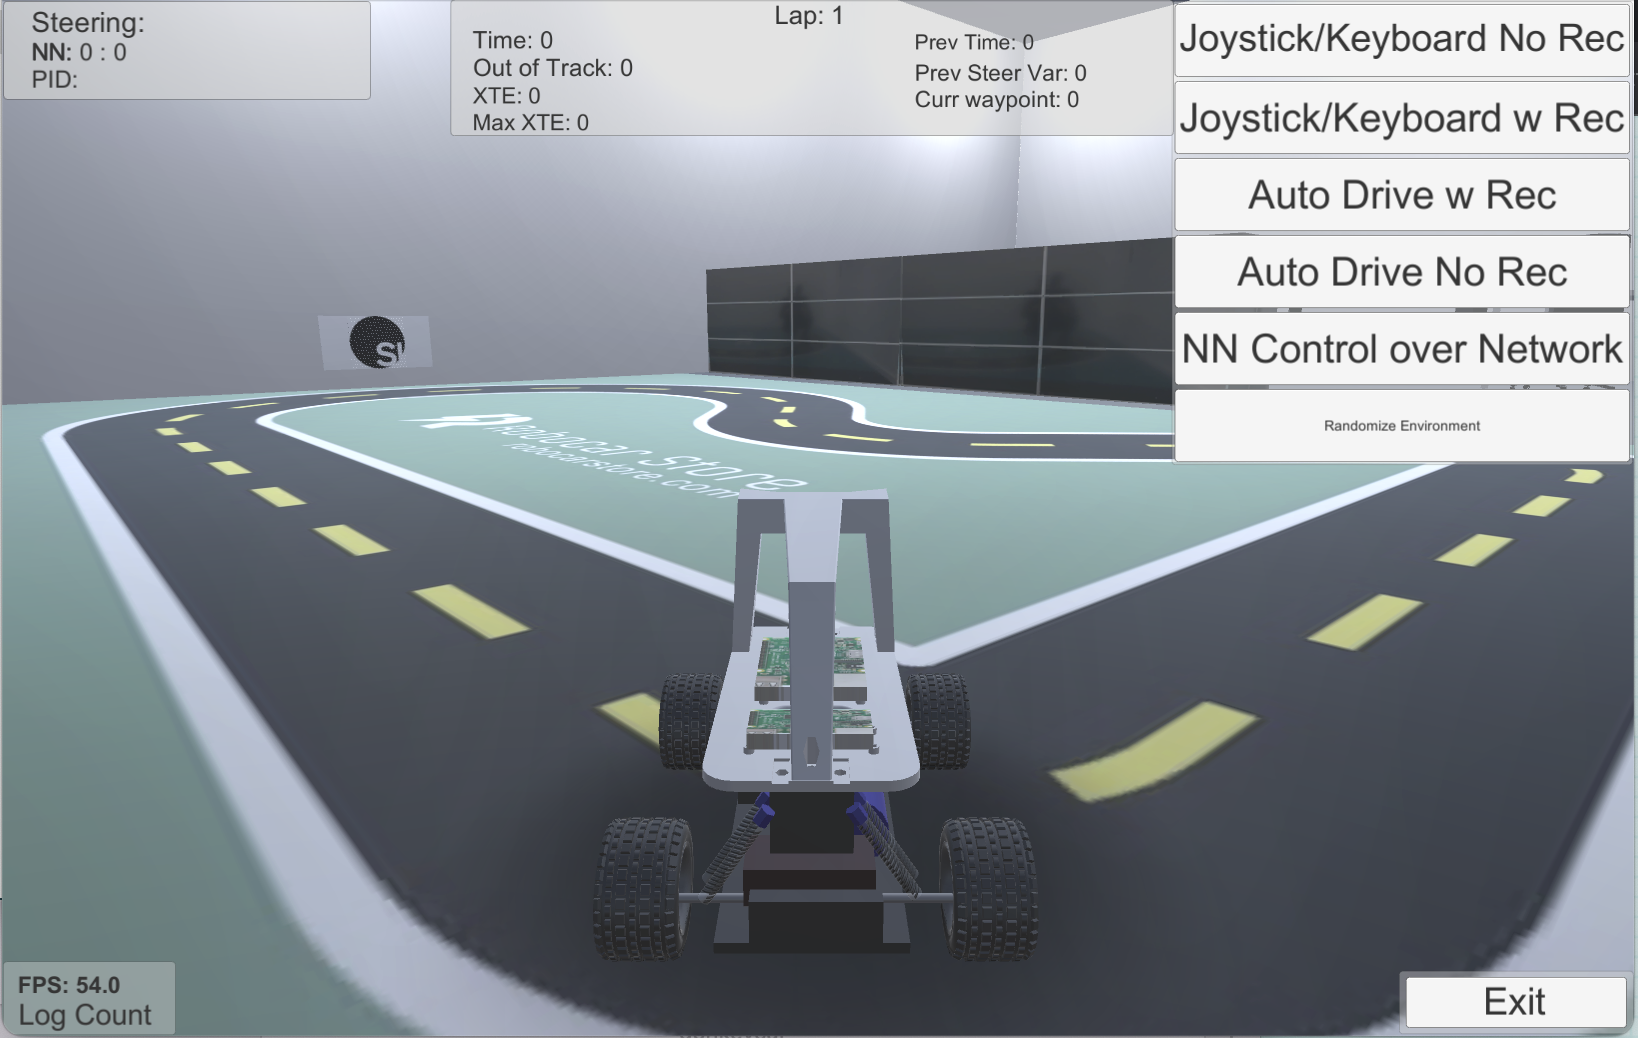
\includegraphics[width=0.6\textwidth]{background/env.png}
  \end{center}
  \caption{DonkeyCar environment implemented with Gym}
  \label{fig:gym}
\end{wrapfigure}

The standard interface designed by Gym, makes it easier to interact with environments, both made available by Gym and externally developed. The Gym interface is simple and capable of representing general RL problems. The DonkeyCar environment, shown in Figure \ref{fig:gym} and used in this piece of work, is an example of what is a custom environment. Gym let us define the action space of the car, which means all the operation it can performs in it such as steer and accelerate. Furthermore, it informs us about the state of the of the car in the environment so that we can perform all the necessary operation, for example, stopping the car when exceeding certain boundaries. 

The documentation provides a reference template shown in Listing \ref{lst:gym} that describes what are the fundamental methods a Gym environment should implement to work properly.
Any existing environment built with Gym implements the following methods:

\begin{center}
  \begin{minipage}{0.45\linewidth}
    \lstinputlisting[caption="Gym template", captionpos=b,  label=lst:gym]{gym.py}
    \end{minipage}
\end{center}

\begin{itemize}
  \item \textbf{init:} every environment should extend the gym.Env class and override the variables \textit{observation\_space} and \textit{action\_space} specifying the type of observations and actions. For example, the observations can be images or continuous vectors as well as actions can be continuous or discrete. According the the Gym notation the state of the environment is called 'observation' since, in general, the state is not fully observable. Therefore, the observation is the observable part of the state, i.e. what the agent can perceive with its sensors.
  \item \textbf{step:} this method is the primary interface between environment and agent, it takes as input the action to be carried out in the environment and return information (observation, reward, done) about the current state such as, the next observation resulting from the action executed in the environment, the corresponding reward value and a boolean flag signaling the end of the 'episode'. Indeed, a Gym environment models episodic RL tasks, i.e. finite tasks that terminate when certain conditions hold.
  \item \textbf{reset:} this method resets the environment to its initial values returning the initial observation. This method is called to initialize the environment and at the end of each episode, such that the agent starts each episode always with a clean state.
  \item \textbf{render:} this method renders the environment when a parameter \textit{mode='human'} is passed.
  \item \textbf{close:} this method performs any necessary cleanup before closing the environment.
\end{itemize}
Besides the API interface, Gym provides a set of wrappers to modify an existing environment without having to change its underlying code directly. The three main things a wrapper does are:

\begin{itemize}
  \item Transform actions before executing them to the base environment
  \item Transform observations that are returned by the base environment
  \item Transform rewards that are returned by the base environment
\end{itemize}
The given set of wrappers to reach any of the aforementioned goal includes: \textit{ActionWrapper}, \textit{ObservationWrapper}, \textit{RewardWrapper}. Furthermore, custom wrappers can be implemented by inheriting from the \textit{Wrapper} class.

\section{Soft Actor Critic - SAC}
The soft actor critic algorithm \citep{art:sac} is a state-of-the-art RL algorithm designed to outperform prior on-policy and off-policy methods in a range of continuous control benchmark tasks. 

It aims to both increase the sample efficiency and the robustness of the policy at test time. A poor sample efficiency is typical of on-policy RL methods since they require new sample to be collected for each gradient step. In order to improve the sample efficiency, SAC adopts an off-policy approach where the experience is stored in a replay buffer such that it can be reused multiple times during training. Moreover, SAC is based on the maximum entropy framework which maximizes both the expected return and the entropy of the policy. This objective is expressed in the following equation:
\begin{equation}
  J(\pi)=\mathbb{E}_{\pi}[\sum _{t=0}^{T}\gamma ^{t}r(s_{t},a_{t})+\alpha H(\pi(\cdot \mid s_{t}))]
\end{equation}
where $\alpha$ is a temperature parameter that weighs the entropy term and thus controls the policy stochasticity, Maximizing both the expected reward and the entropy of the policy is beneficial to obtain policies that are robust w.r.t. unexpected situations at testing time. Moreover, training a stochastic policy encourages a wide exploration of the environment, promoting diverse behaviors of the agent.

\section{Generative Adversarial Networks - GAN}
\begin{wrapfigure}{r}{0.6\textwidth}
  \begin{center}
    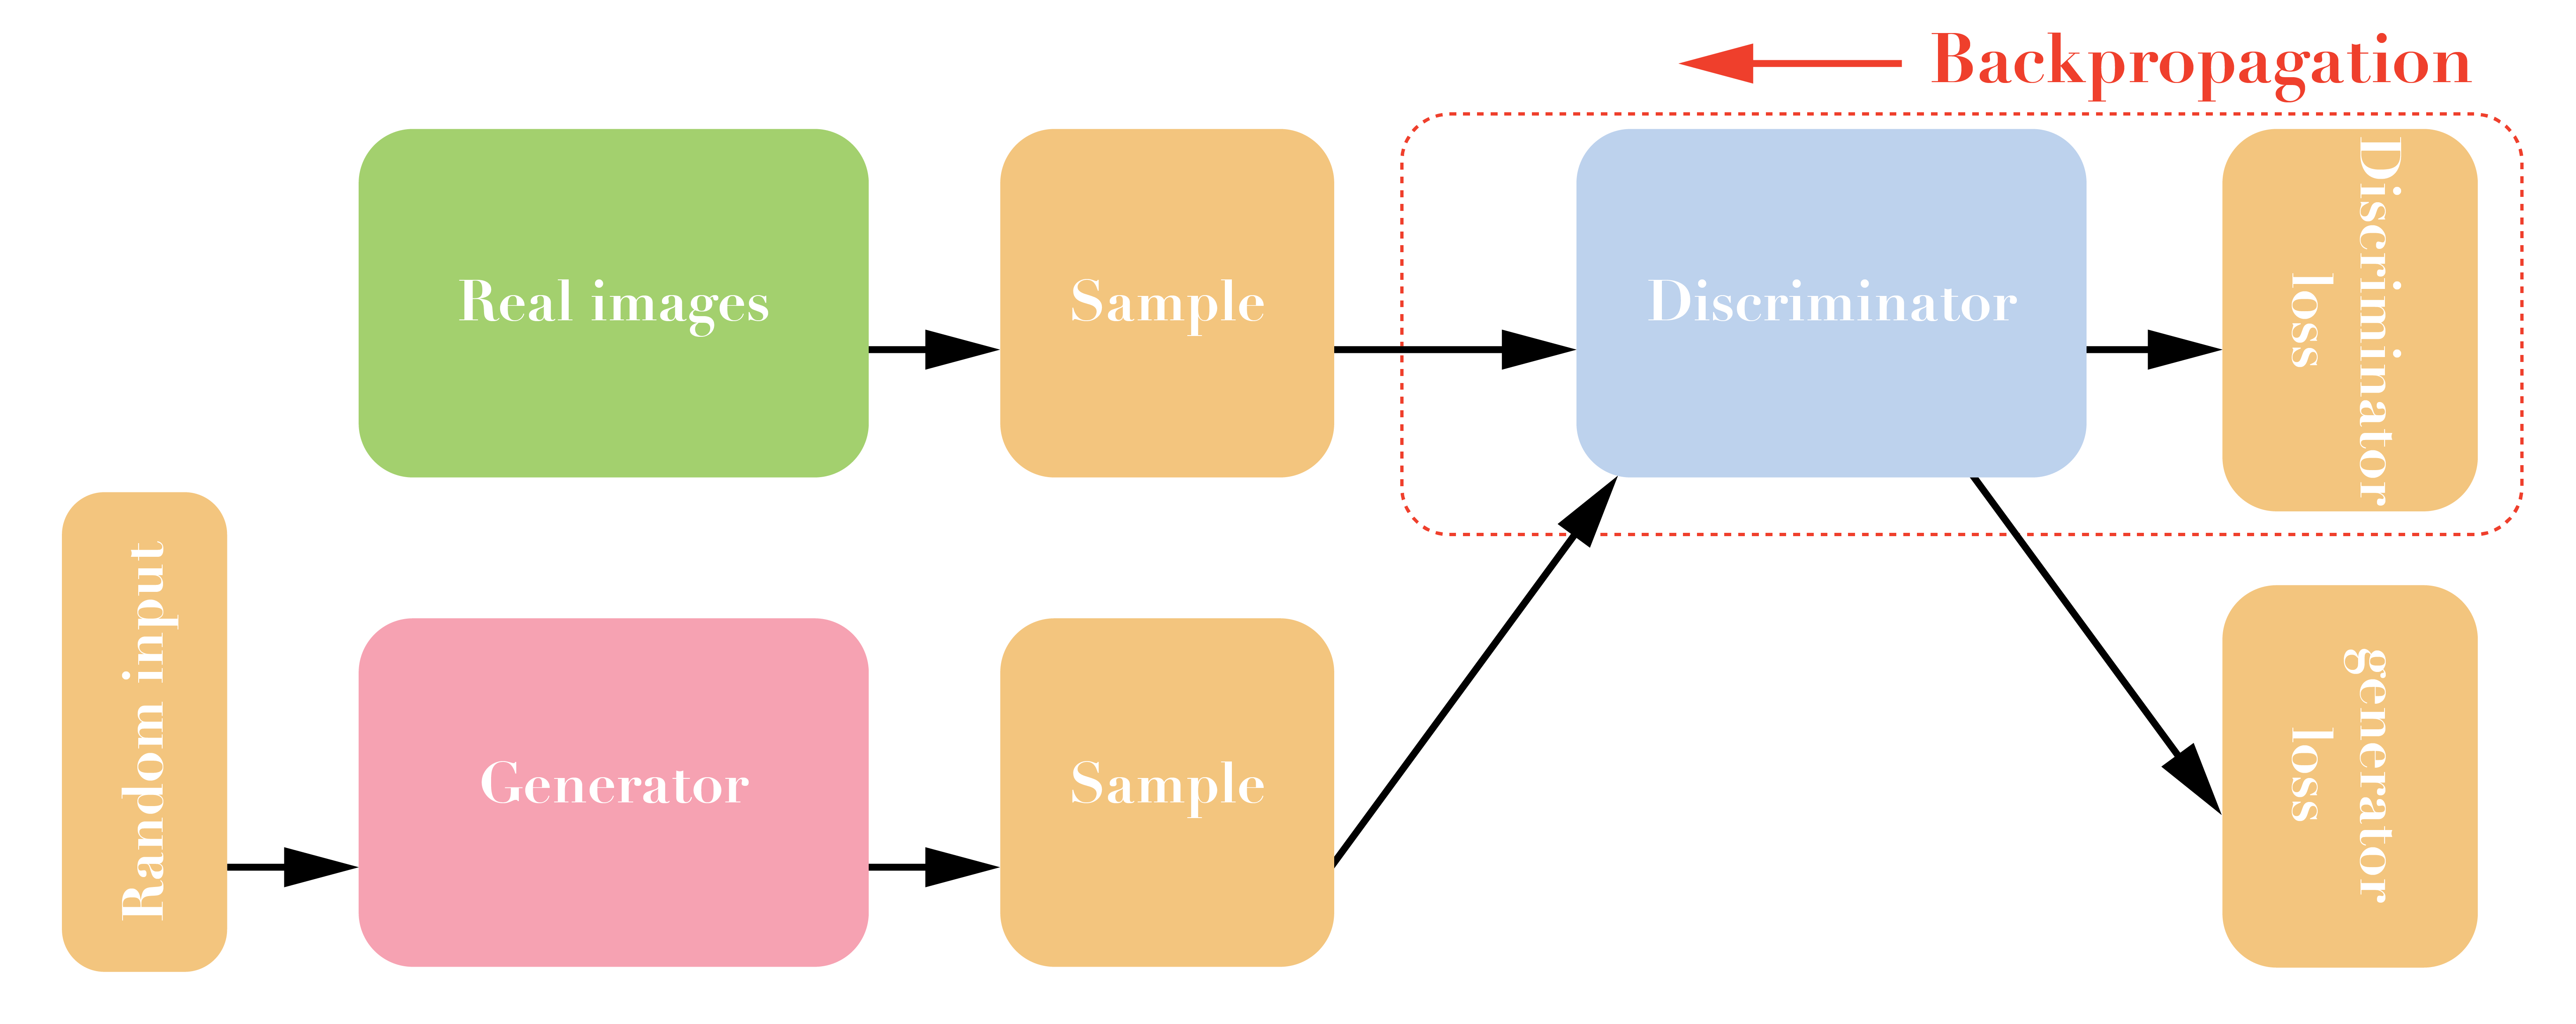
\includegraphics[width=0.6\textwidth]{background/gan.png}
  \end{center}
  \caption{GAN diagram}
  \label{fig:gan}
\end{wrapfigure}

Generative Adversarial Network is a framework introduced by \citet{art:gan} for training generative models in an unsupervised fashion. GANs can be used, for example, to generate visual paragraph \citep{Liang_2017_ICCV}, realistic text \citep{pmlr-v70-zhang17b}, photographs of human faces \citep{https://doi.org/10.48550/arxiv.1710.10196} and Image-to-Image translation \citep{Isola_2017_CVPR}.
The learning process involves two neural networks that are trained in an adversarial way, i.e. with a contrasting objective. Indeed, as shown in Figure \ref{fig:gan}, the generator G generates inputs (e.g images) starting from random noise and the discriminator D needs to distinguish whether such inputs belong to the original dataset or not. GANs fall under the branch of unsupervised learning since the training process does not need labeled data as the generator is guided by the discriminator in order to generate inputs that resemble those of the training dataset. The discriminator $D$ is trained to maximize the probability of returning the correct label when given both training examples and examples generated by the generator $G$. At the same time the objective of generator $G$ is to minimize the following loss function:
\begin{equation}
  \label{eq:gloss}
  L_G =log(1-D(G(z)))
\end{equation}
where $z$ is the random noise vector, i.e. the latent vector, $D(G(z))$ is the probability that the generated example $G(z)$ comes from the training dataset (represented by the distribution $p_{x}$ where X is the training dataset and $p_{x}$ represents all the possible images that can be in X), which means that $1-D(G(z))$ is the probability that $G(z)$ does not come from from $p_{x}$. Indeed, the objective of the generator $G$ is to generate examples that are indistinguishable from the training examples for the discriminator $D$.

In particular, in order to learn the generator's distribution $p_{g}$ over the training dataset $X$ such that $p_{g}\approx p_{x}$, the authors define a distribution over latent vectors $p_{z}(z)$, which is mapped into the data space with the generator $G(z, \theta_{g})$. Moreover, the discriminator $D(x;\theta_{d})$, with $x \sim p_{g}$, outputs a single value which estimates the probability of $x$ coming from the distribution $p_{x}$ rather than $p_{g}$. $D$ and $G$ are both differentiable functions represented by a neural network with parameters $\theta_{d}$ and $\theta_{g}$ respectively.

In other words, the discriminator and the generator play a minimax game to optimize the function $V(G,D)$:
\begin{equation}
  \label{eq:ganloss}
  min_G max_D V(G,D) = \mathbb{E}_{x\sim \rho_{data}(x)}[log D(x)] + \mathbb{E}_{z\sim \rho_{z}(z)}[log (1-D(G(z)))]
\end{equation}

\section{CycleGAN}
Image-To-Image translation is a complex task where the goal is to transform an image from one domain to another and vice-versa, as shown in Figure \ref{fig:translation}.
\begin{wrapfigure}{r}{0.5\textwidth}
  \begin{center}
    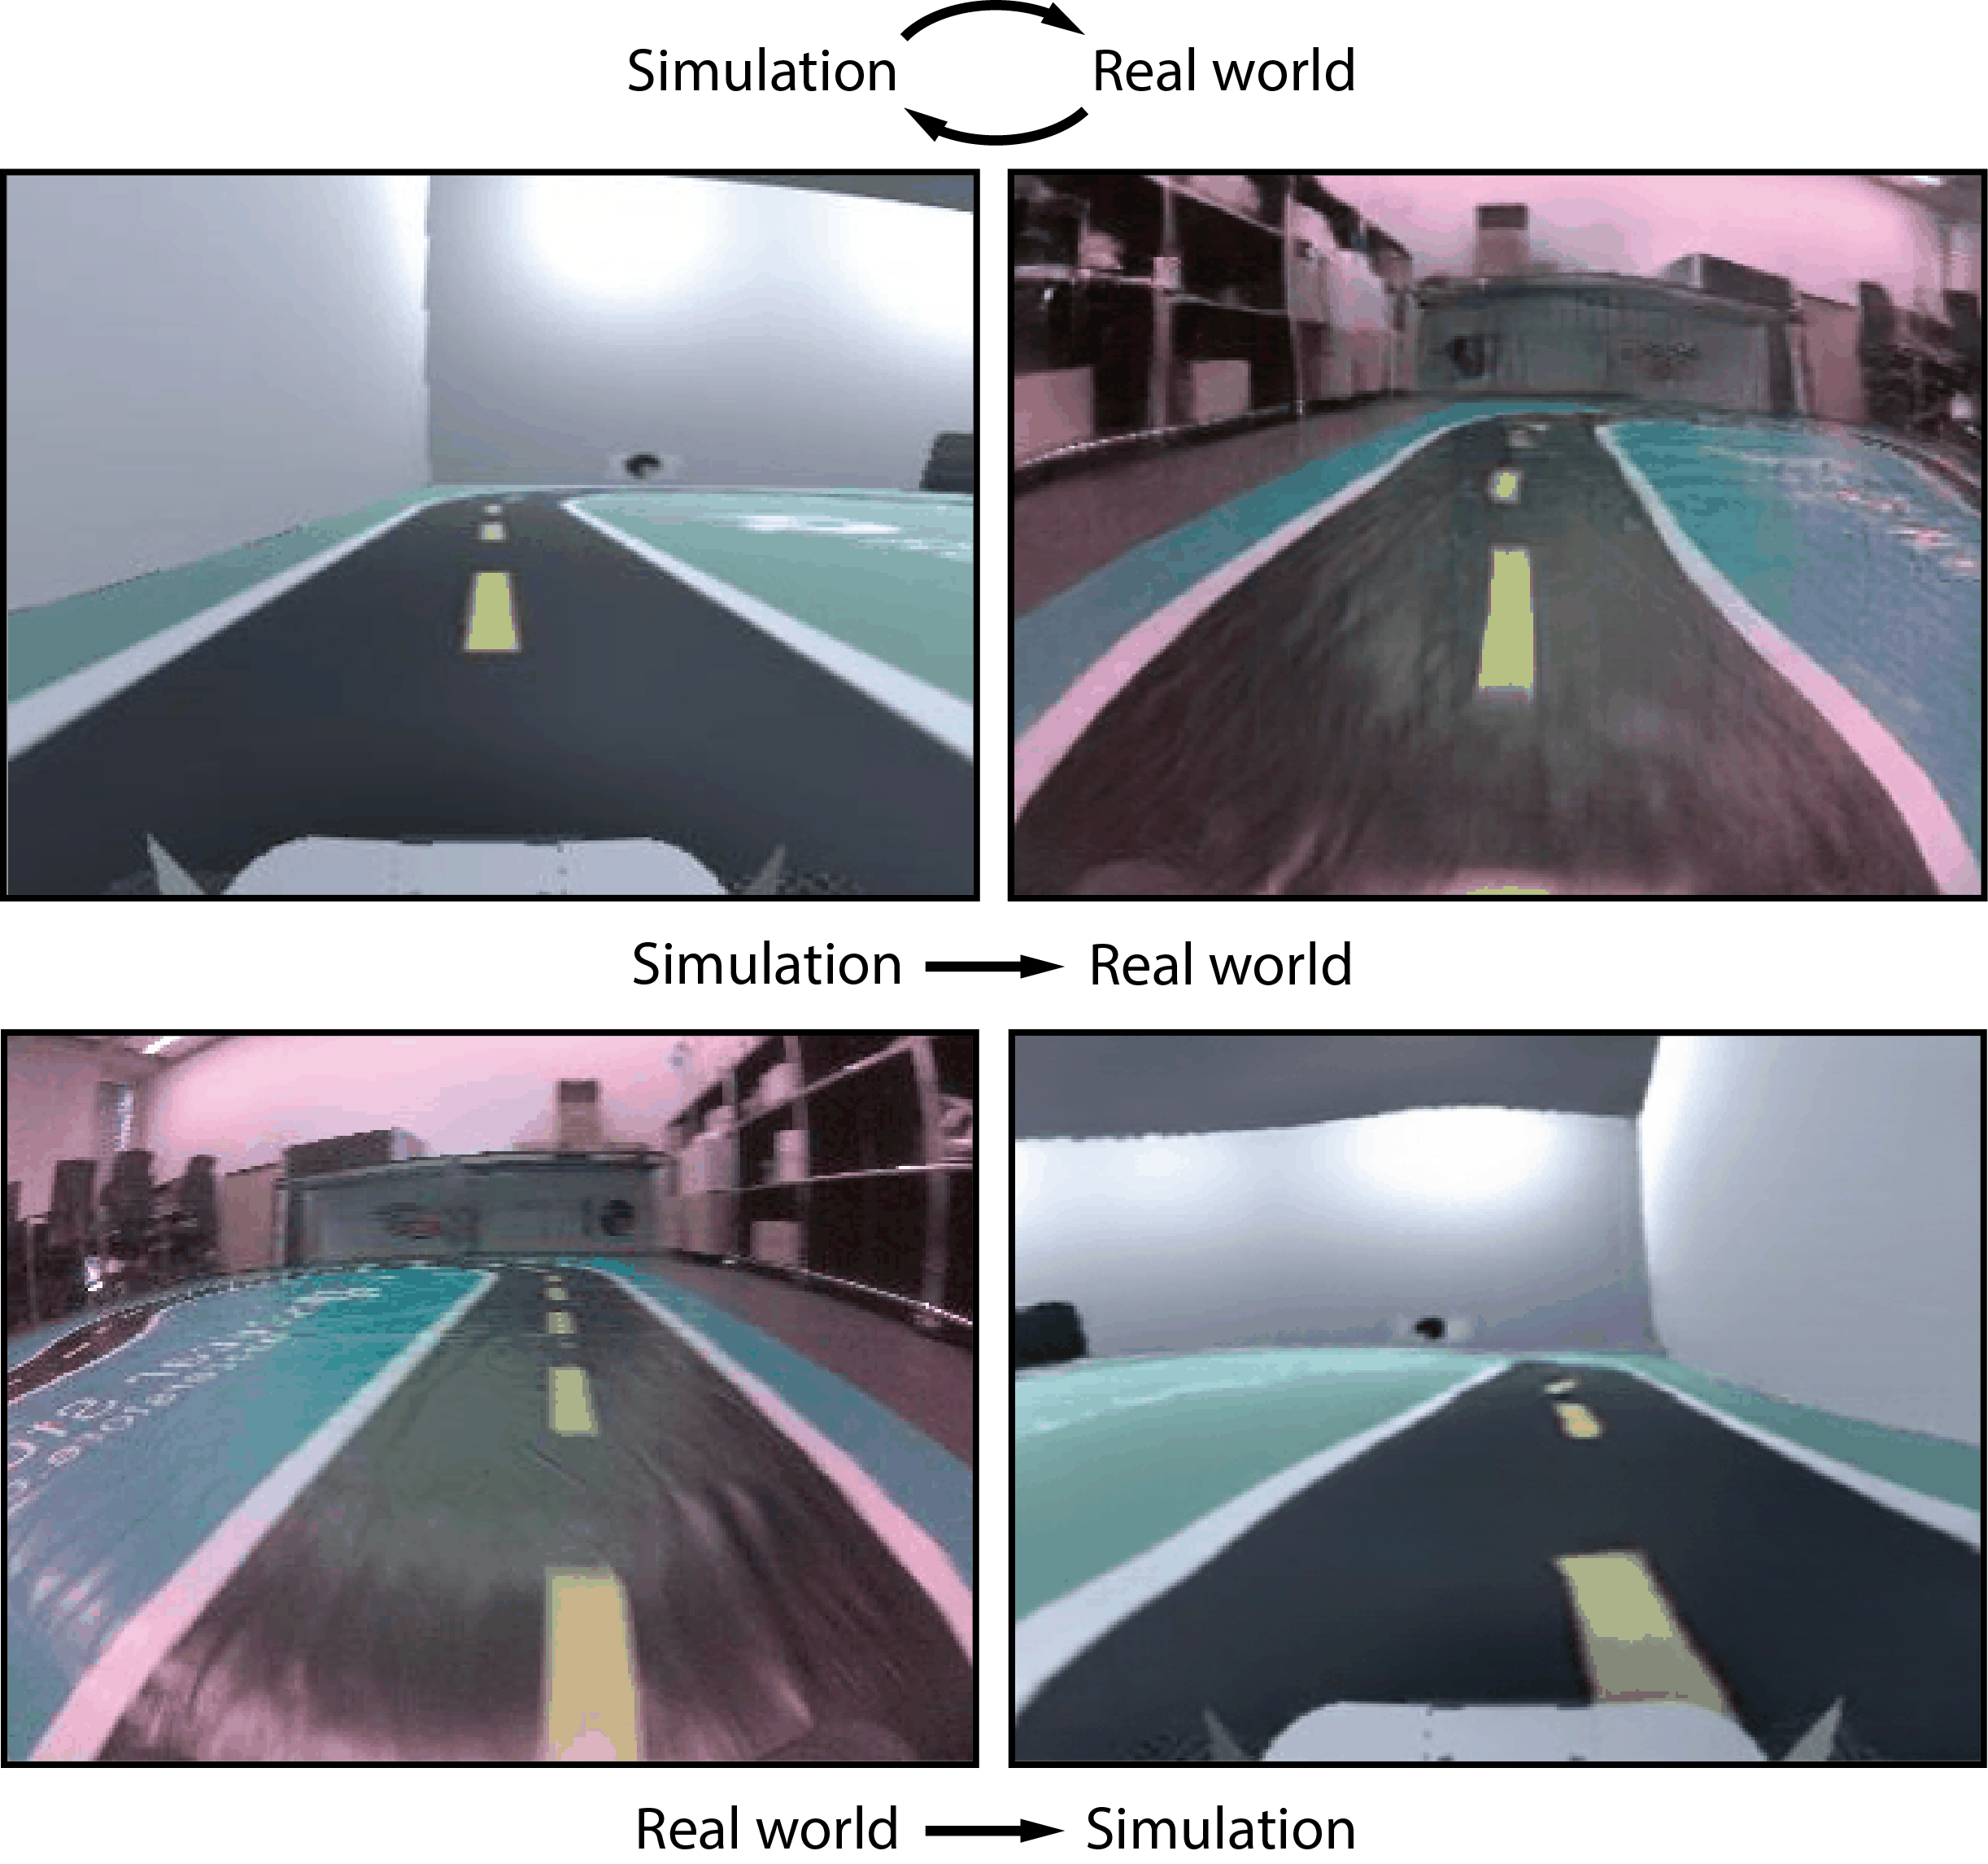
\includegraphics[width=0.5\textwidth]{background/imagetranslation.png}
  \end{center}
  \caption{Image-to-image translation example \citep{CycleGAN2017}.}
  \label{fig:translation}
\end{wrapfigure}
Prior papers have been presented to translate images, however they often require paired training examples between the domains [\citet{https://doi.org/10.48550/arxiv.1612.00835}, \citet{karakan}].
Such paired datasets can be very expensive or even impossible to gather, as in the case of object transfiguration ($horse \leftrightharpoons zebra$).

Cycle-Consistent Adversarial Networks from \citet{CycleGAN2017} (CycleGAN), aims to solve this problem in an unsupervised fashion. The main goal is to learn, using an adversarial loss, a mapping $G:X\rightarrow Y$, where $X$ and $Y$ are two sets representing different domains, such that the image $G(x) $ with $x\in X$ is indistinguishable from an image $y\in Y$. Since the mapping is highly under-costrained, an inverse mapping $F:Y \rightarrow X$ is introduced, together with a cycle-consistency loss to enforce $F(G(x)) \approx x$ and vice-versa.
To accomplish the goal two discriminator $D_{X}$ and $D_{Y}$ are provided. $D_{X}$ tries to distinguish between examples coming from one domain (i.e. represented by the distribution $\rho_{x}$) and their translations $F(Y)$ and vice-versa for $D_{Y}$. 
The full objective \ref{eq:cycleganloss} includes the adversarial losses and the cycle-consistency loss to encourage a consistent translation from one domain to the other:
\begin{equation}
  \label{eq:cycleganloss}
  L(G,F,D_{X}, D_{Y}) = L_{GAN}(G, D_{Y},X,Y) + L_{GAN}(F, D_{X},Y,X) + \lambda L_{cyc}(G,F)
\end{equation}
where the loss $L_{GAN}(G, D_{Y},X,Y)$ and $L_{GAN}(F, D_{X},Y,X)$ can be constructed from Equation in \ref{eq:ganloss}
% where the loss $L_{GAN}(G, D_{Y},X,Y)$ is described below and $L_{GAN}(F, D_{X},Y,X)$ can be derived similarly:
% \begin{equation}
% L_{GAN}(G, D_{Y},X,Y) = \mathbb{E}_{y\sim \rho_{data}(y)}[log D_{Y}(y)] + \mathbb{E}_{x\sim \rho_{data}(x)}[log (1-D_{Y}(G(x)))]
% \end{equation}
and the following is the cycle-consistency loss:
\begin{equation}
  L_{cyc}(G,F) =  \mathbb{E}_{x\sim \rho_{x}}[\left \| F(G(X))-x \right \|_1] + \mathbb{E}_{y\sim \rho_{y}}[\left \| G(F(y))-y \right \|_1]
\end{equation}
where $\lambda$ is a temperature parameter to define the importance of such loss in Equation \ref{eq:cycleganloss} and $\| \cdot \|_1$ is the L1 norm, i.e. a measure of the distance between vectors.

\section{AutoEncoder and Variational AutoEncoder}

\subsection{AutoEncoder}
AutoEncoders (AEs) are artificial neural networks that fall under the branch of unsupervised learning since they learn efficient encoding into a latent space without the need of a labeled dataset. They are generally used for several purposes, for example, dimensionality reduction, image compression, image denoising, image generation, feature extraction and sentence generation [\citet{doi:10.1126/science.1127647}, \citet{8456308}, \citet{7836672}, \citet{7926714}, \citet{8852155}]. 

Taking as example the case of image dimensionality reduction, an AE is composed of two main parts, an encoder $E$ and a decoder $D$. 
\begin{align}
  E(\phi) &:  X \rightarrow Z & D(\theta) &:  Z \rightarrow X'
\end{align}
where $X = \mathbb{R}^{mxn}$ and $Z = \mathbb{R}^{k }$ for some $m,n,k$ and $k\ll mxn$ to reach the goal of dimensionality reduction. Both encoder and decoder are parametrized functions, with parameters $\phi$ and $\theta$ respectively,
As shown in Figure \ref{fig:ae}, the main goal of the encoder is to learn a mapping of each observation of the dataset $x \in X$ into a latent space of smaller dimensionality.  Since a label is not available, in order to measure the quality of the embedded image into the latent space, the decoder is used to reconstruct the image and then compute the reconstruction loss.

\begin{figure}[h]
  \begin{center}
    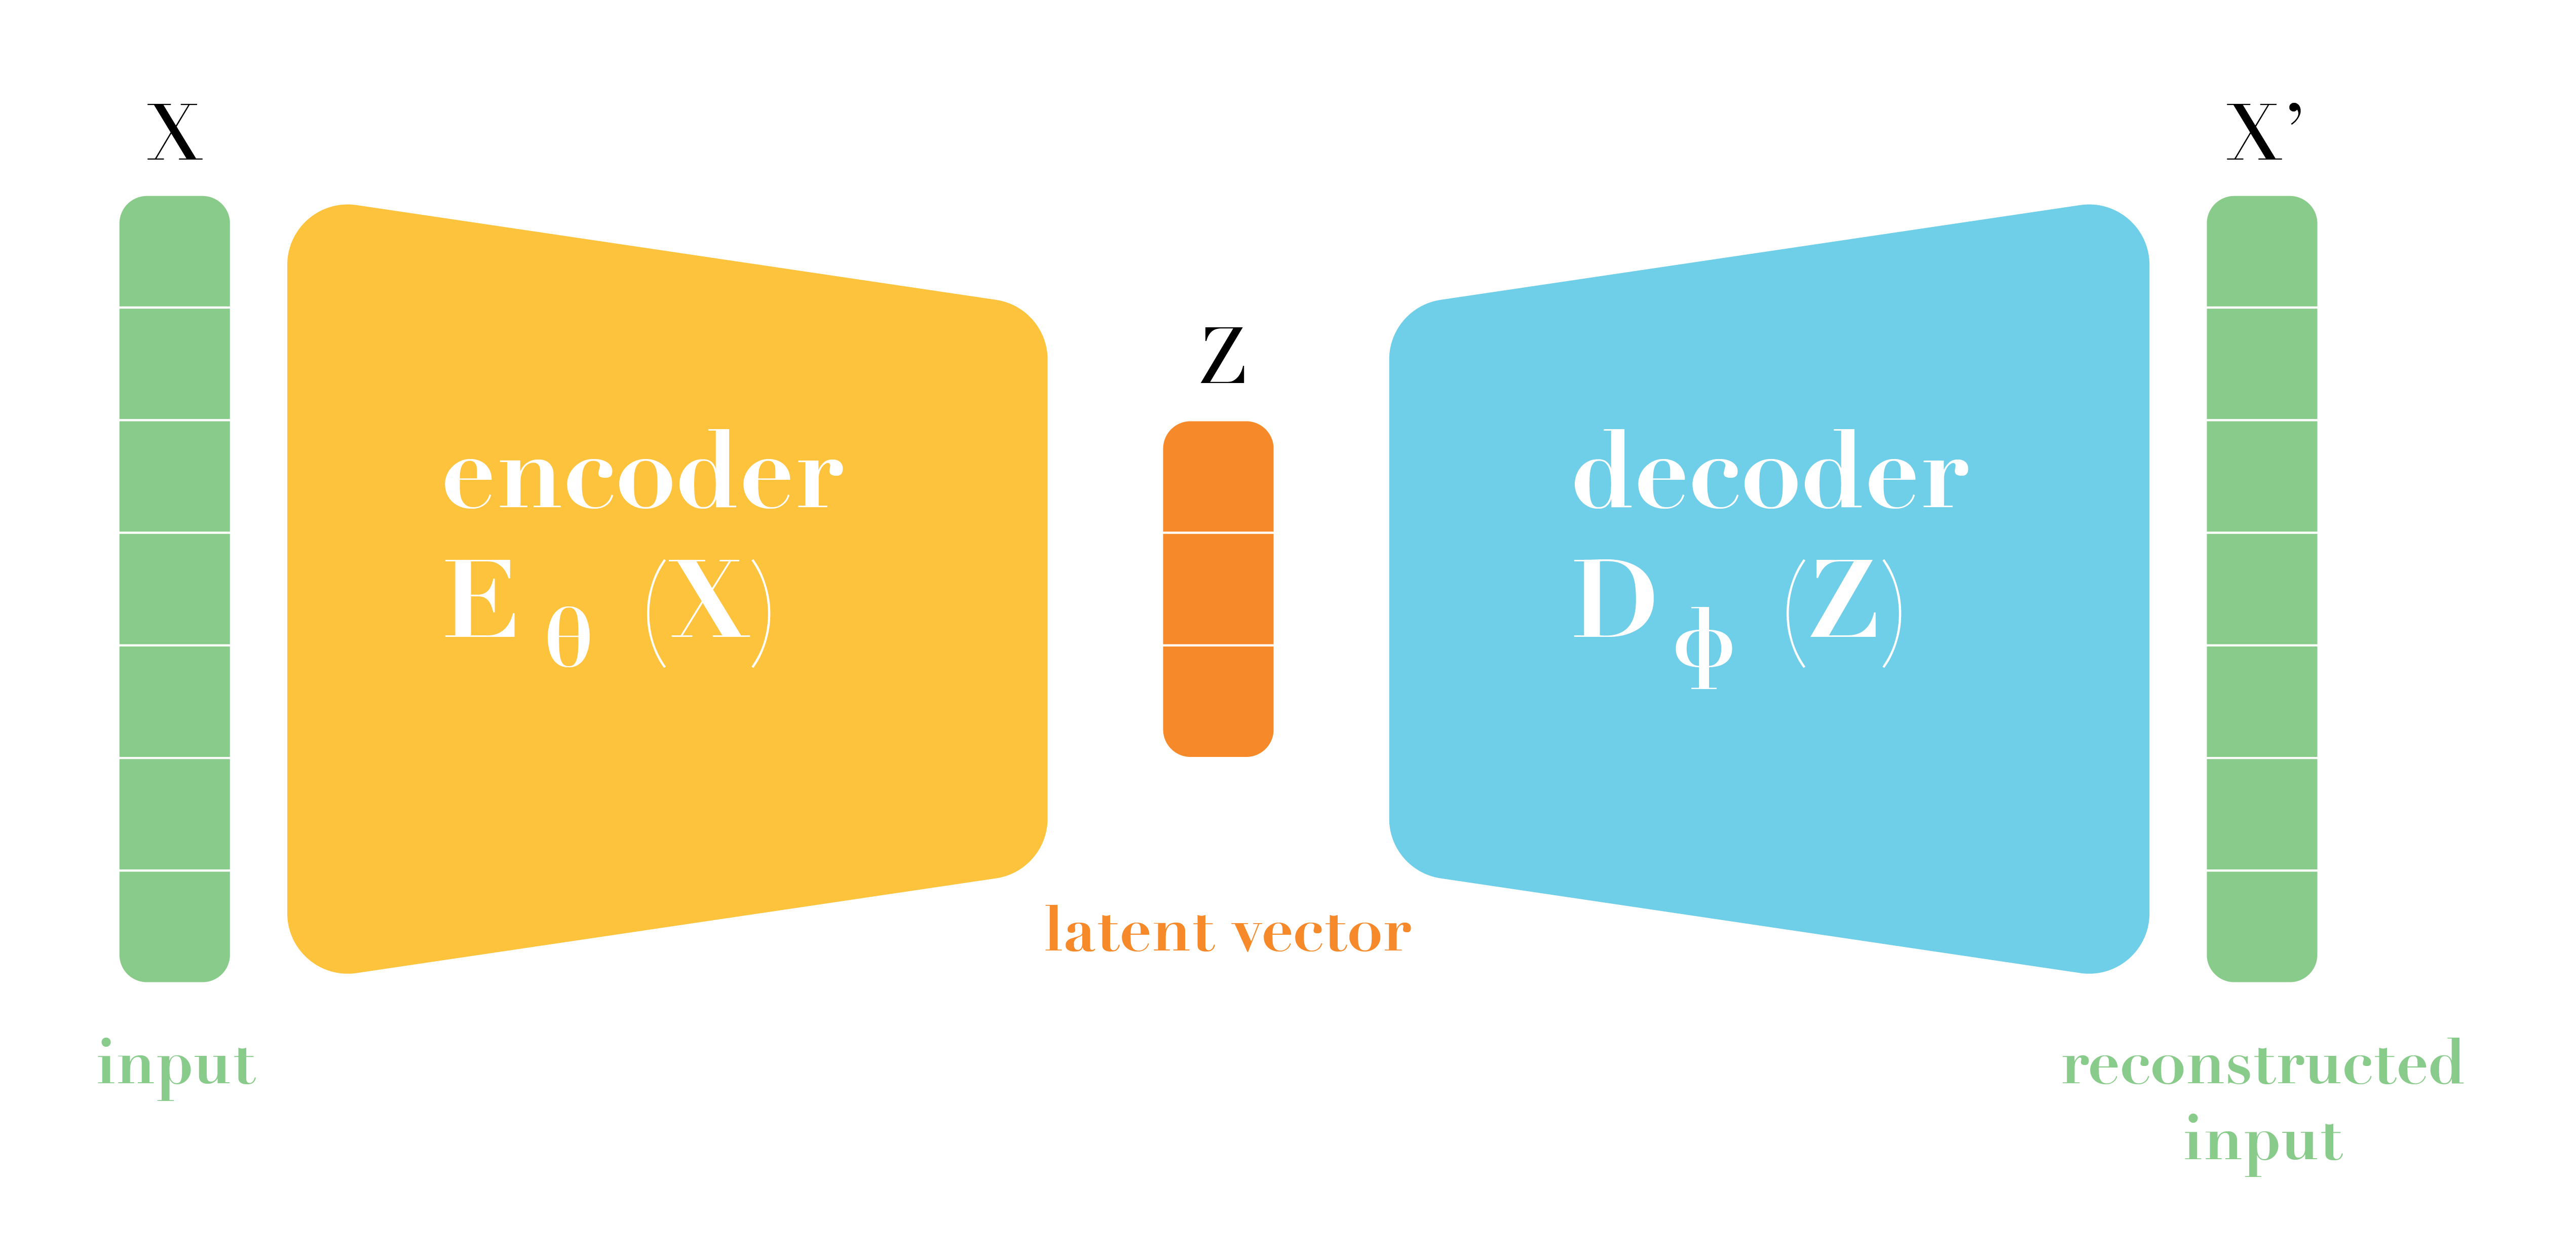
\includegraphics[width=0.70\textwidth]{background/ae.png}
  \end{center}
  \caption{AE diagram}
  \label{fig:ae}
\end{figure}

In other words, the encoder maps an image $x\in X$ into the latent space producing ${z=E_{\phi }(x)}$ with $z\in Z$; then $z$ is reconstructed by the decoder to bring it back to the original space ${x'=D_{\theta }(z)}$ with $x'\in X'$. Finally, $x'$ can be used as a label with any distance measure $d(x,x')$. Thus the loss to be minimized is computed as follows:

\begin{equation}
\label{eq:aeloss}
  L(\theta ,\phi ) = d(x_{i},D_{\theta }(E_{\phi }(x_{i})))
\end{equation}

\subsection{Variational AutoEncoder}

Variational AutoEncoders (VAEs) addresses the problem of \textit{sparse localization} of data point into the latent space thus providing a more powerful generative capability then AEs.

\begin{figure}[h]
  \begin{center}
    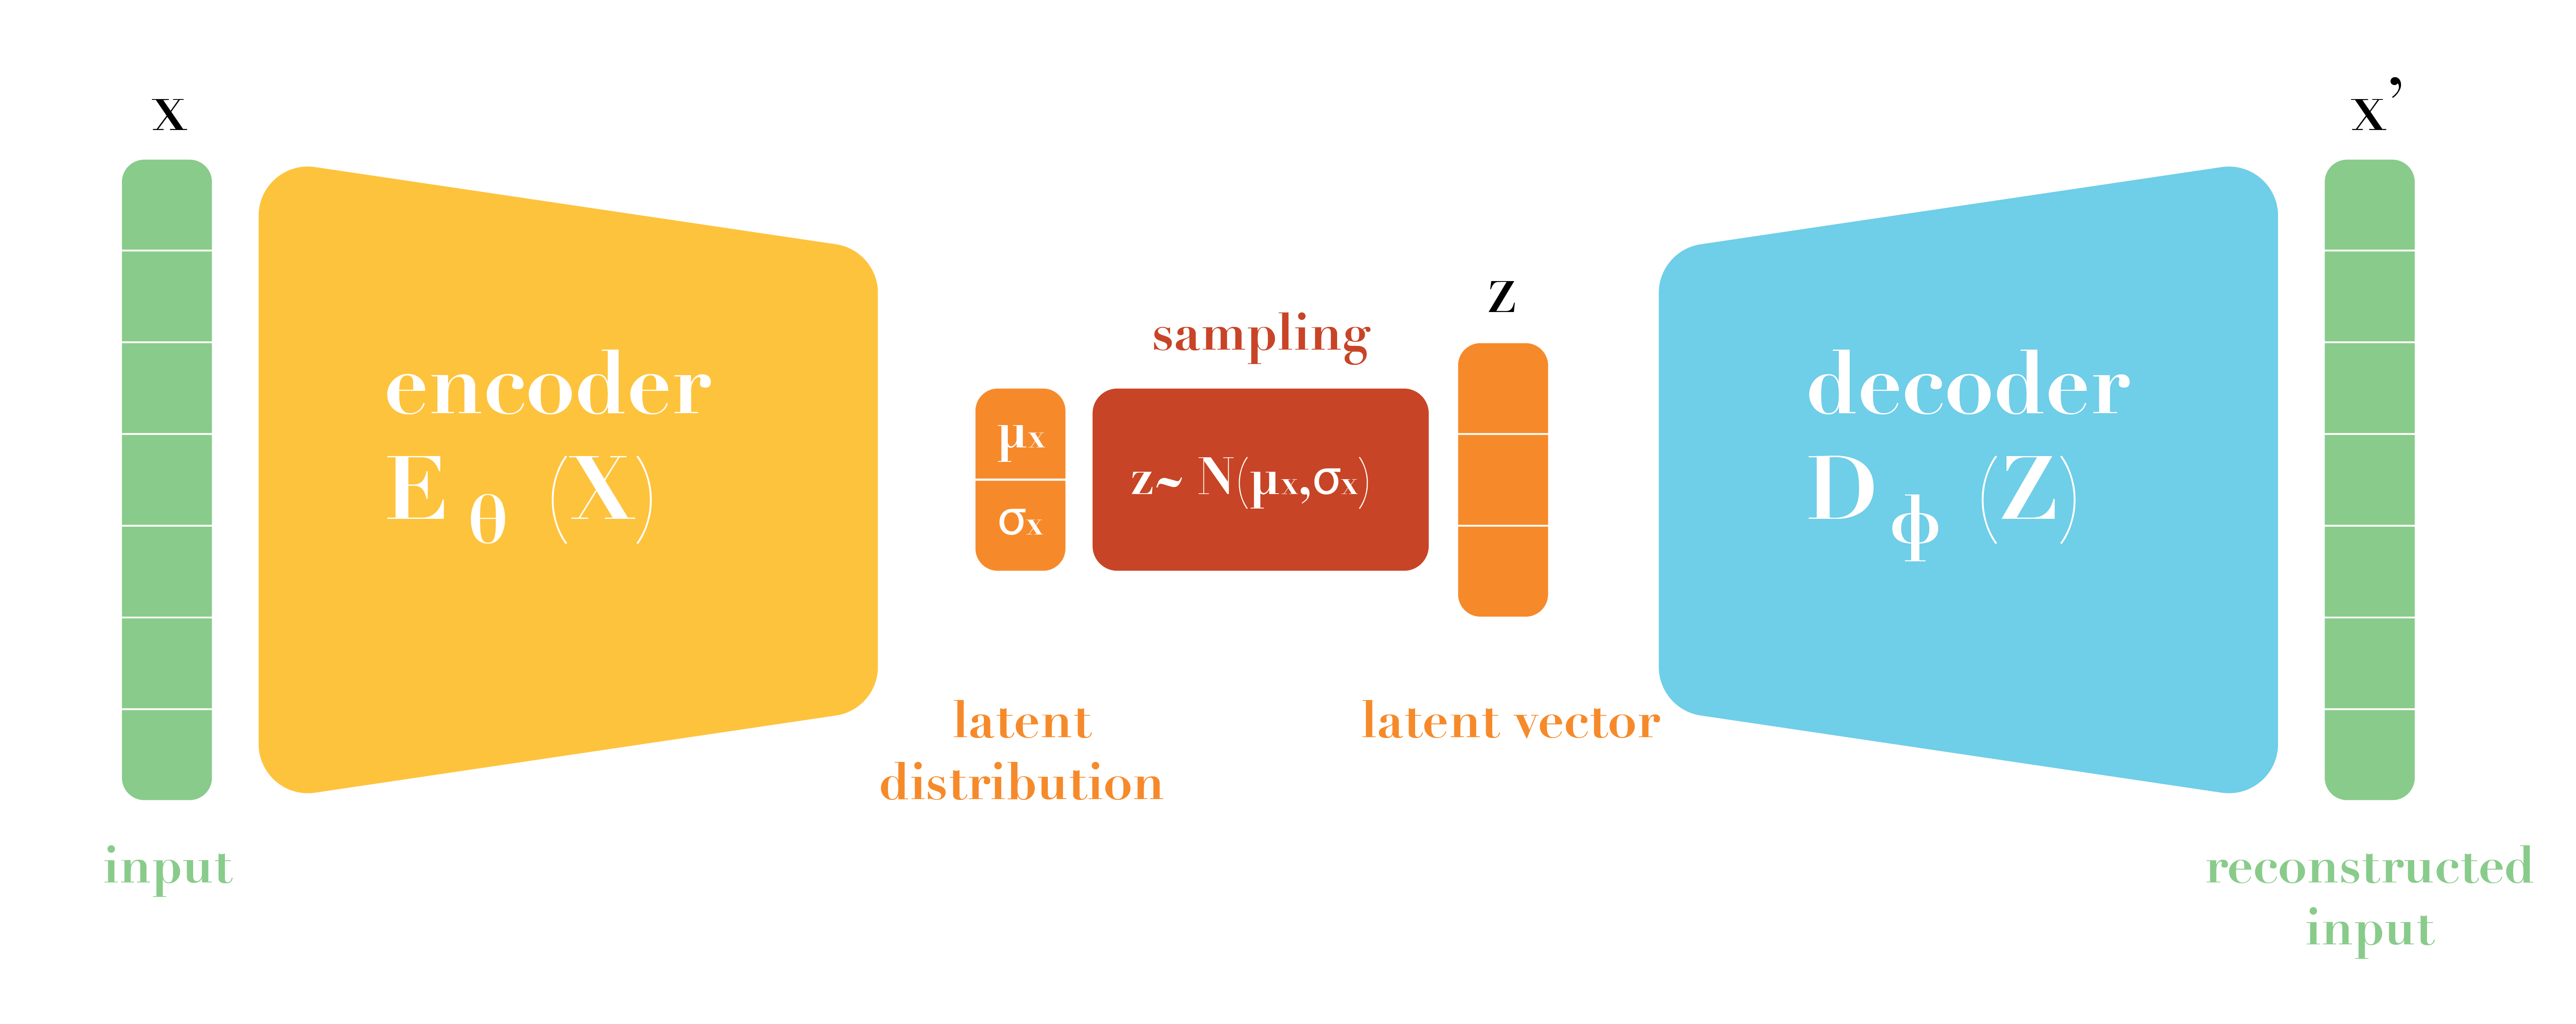
\includegraphics[width=0.80\textwidth]{background/vae.png}
  \end{center}
  \caption{VAE diagram}
  \label{fig:vae}
\end{figure}

As shown in Figure \ref{fig:vae} only a small change with respect to AEs is introduced, i.e. the encoder instead of mapping samples directly into the latent space it encodes a single input as a distribution (usually a normal distribution) over the latent space. Then the concrete latent vector $z$ is produced by sampling such distribution. 

Specifically, the encoder, starting from an image $x\in X$, produces the gaussian parameters ${[\mu_x, \sigma_x]=E_{\phi }(x)}$, then $z$ is sampled from a normal distribution $z \sim \mathcal{N}(\mu_x, \sigma_x)$. Consequently, the decoder brings it back to the original space ${x'=D_{\theta }(z)}$ with $x'\in X'$. Finally, $x'$ can be used as a label with any distance measure $d(x,x')$. Thus the loss to be minimized is computed as follows:
\begin{equation}
\label{eq:vaeloss}
  L(\theta ,\phi) = d(x_{i},D_{\theta }(E_{\phi }(x_{i}))) + KL[\mathcal{N} (\mu_x, \sigma_x),\mathcal{N}(0, 1)]
\end{equation}
where the first term is equivalent to the loss function in Equation \ref{eq:aeloss} and the KL term is the Kullback-Leibler divergence, which is a measure of how a probability distribution is different from another. The KL divergence acts as a regularization term by enforcing predicted distributions to be close to the normal distribution with mean 0 and standard deviation 1, giving to the latent space two main properties, i.e. continuity (close points in the latent space should be close also when decoded) and completeness (any point sampled from the latent space should always be meaningful once decoded). 

\section{DonkeyCar} \label{sec:donkeycar}
DonkeyCar, shown in Figure \ref{fig:donkey}, is an open source DIY platform providing software and hardware tools for the development of self-driving car algorithms. The basic car is a simple remote controlled electric car that can be 3D printed or bought as a kit for an affordable price. The car can be customized with additional sensors as LIDARs and IMUs to provide more information about the surroundings of the car during driving.

\begin{wrapfigure}[19]{r}{0.5\textwidth}
  \begin{center}
    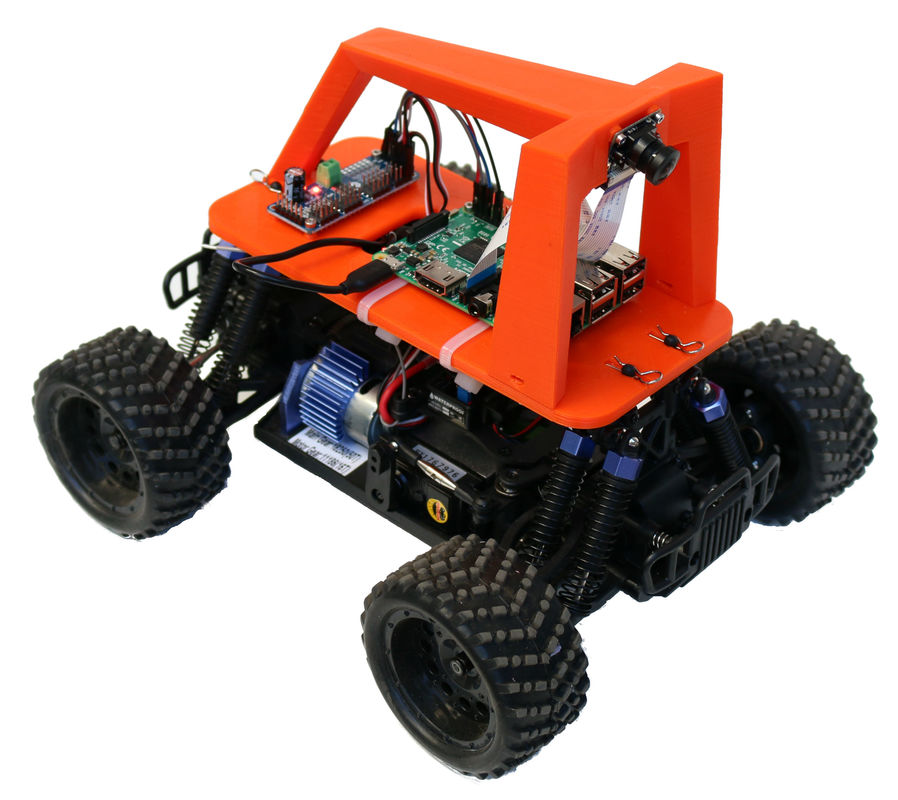
\includegraphics[width=0.5\textwidth]{background/donkey.jpeg}
  \end{center}
  \caption{Assembled DonkeyCar}
  \label{fig:donkey}
\end{wrapfigure}

In particular, the car used for the purposes of this thesis, is a basic donkey car equipped with an 8-megapixel IMX219 sensor that features an 160 degree field of view. It is capable of capturing images with a resolution of 3280x2464 and video recording up to a resolution of 1080p at 30 frames per seconds. In order to process all the information coming from the camera, control the motors and run the self-driving car software the car is equipped with an NVIDIA Jetson Nano micro-controller. The power comes from a LiPO battery of 11.1V and 2200mAh that runs the electric motor and the micro-controller. Additionally, to expand the operational life of the car, a power-bank can be added to exclusively power the micro-controller, while the LiPO battery is dedicated at powering the engine. 
A DonkeyCar can be remotely controlled either with a joystick or directly by the software.
\chapter{Related works}

When training a Reinforcement Learning model there are several problem that can arise and need to be tackled, especially when the learning process moves from simulated environments to the real world. In this section a few methods, particularly useful for the purposes of this thesis, are presented.

\section{State Representation Learning} \label{sec:srl}

Reinforcement Learning is a very general method for learning sequential decision making tasks. On the other hand, Deep Learning has become in recent years the best set of algorithms capable of Representation Learning (ReL). Representation learning algorithms are designed to extract abstract features from data. A mix of the two provides a particularly powerful framework for learning state representation, especially when dealing with real world environments that tend to be much more complex and unpredictable than simulated environments. In particular, State Representation Learning (SRL) is a specific type of ReL where extracted features are in low dimension, evolves in time and are affected by an agent's action. The low dimensionality allows easier interpretation by humans, helps in handling the curse of dimensionality and speeds up the policy learning process. Thus, SRL is well suited for Deep Reinforcement Learning applications. \citet{DBLP:journals/corr/abs-1802-04181} presented a complete survey that covers the state-of-the-art on SRL. Feature extraction and learning is a wide topic that tries to discover features that characterize data by decomposing them. Taking as example a dataset of portraits, a set of features that can compose each picture can be the hair color, skin color, face shape and so on. Training a neural network to learn those features may be accomplished by compressing the image into a smaller vector, discarding all the useless informations for the model, where each dimension would represents a feature like the ones just described. However, a feature not necessarily describes a humam readable aspect of the data but can be even without a semantic meaning. In particular, SRL exploits the time steps, actions, and eventually rewards, to transform observations into states, a low dimensionality vector that contains the most relevant features to learn a particular policy that acts as a supervisor. The better the policy or the speed with which it is learned, the more the features extracted are significant to the model.

\section{Improving sample efficiency} \label{sec:sampleefficiency}

In order to define the state of the environment in our experiment we use a camera as described in Section \ref{sec:donkeycar}. However, training a model from high-dimensional images with reinforcement learning is difficult, in previous Section \ref{sec:srl} we described an approach to mitigate those difficulties. In this section we present a specific method that is used for the purposes of this thesis.

Deep convolutional encoders can learn a good representation even though they generally require large amounts of training data. Using off-policy methods and adding an auxiliary task with an unsupervised objective can naturally improve sample efficiency and add stability in optimization but they often lead to suboptimal policies as described in \citet{DBLP:journals/corr/abs-1910-01741}. They revisit the concept of adding an encoder to off-policy RL methods and provide a simple and  effective autoencoder-based off-policy method that can be trained end-to-end. The main focus is in finding the optimal way of training a RL agent using SRL.

In practice, in their experiment, the AE is composed of a convolutional encoder that maps an image observation to a low dimension vector into the latent space and a deconvolutional decoder the reconstruct the latent vector back to the original image. While several auxiliary objectives could be used to improve the learned representation, they target on the most general and widely applicable, an image reconstruction loss avoiding task dependent losses. After that, a SAC algorithm is used to learn some task from the latent state of the environment.

There are two options, the first one seeks to train the agent alternately with the encoder with both kept indipentent from each other. So the AE is pretrained and then a few iteration are used to improve the AE with its own loss, later on, the agent is trained with the encoder kept constant. The algorithm keeps iterating between this two phases until convergence. The second option, seeks to learn a latent representation that is well aligned with the underlying RL objective, thus the AE network is updated with the gradient coming from the actor, critic and the AE itself. However, this attempt of joint representation learning was proven unsuccesful. For this reason, our focus is on the first alternating representation learning. The last thing to define is how often the encoder should be updated. From the tested tasks is evident that it should be updated at the end of every episode, however, even if it is never updated after the first pre-training, the result are still very good. Beside that, an on going update would require more computational power to complete all the algorithm steps in the same amount of time. Since this work aims to solve a real-time problem, it is necessary that a certain number of frames are processed per second that is why the single pretrain is preferable in the context of microcontroller, PC without a GPU and over-the-air communication. Even though this could lead to a slightly longer training, it would speed up the single iteration.

\section{Smooth exploration}

When moving a RL algorithm from a simulated environment to the real world, the unstructured step-based exploration often very successful in simulation, leads to unstable motion patterns. This may results in poor exploration, longer training and even damages to the robot's motors that can be expensive. \citet{pmlr-v164-raffin22a} handle the issue by including a state-dependent exploration (SDE) to current Deep Reinforcement Learning algorithms. In most RL algorithm the standard for exploration is to sample a noise vector from a Gaussian distribution indipendent from the environment and the agent, and then it is added to the controller output. SDE replaces the sampled noise with a state-dependet exploration function. This results in smoother exploration and less variance for each episode. In practice the solutions is as simple as sampling a noise vector as a function of the actual state $s_t$ and adding it to the choosen action.

\section{Learning to Drive - L2D}
Learning to Drive (L2D) \citep{DBLP:journals/corr/abs-2008-00715} is a low-cost benchmark for real world autonomous driving learned through reinforcement learning. Since training this types of RL algorithms can be very expensive due to the nature of trial-and-error learning and the cost of a real car, the benchmark are carried out using a DonkeyCar as described in Section \ref{sec:donkeycar}. The authors also provide the source code in order to let every one implent his own RL algorithm to solve DonkeyCar autonomous driving task which we, for the sake of simplicity, use as a baseline of our experiments. They demonstrate that existing RL
algorithms, like Imitation learning, SAC+VAE and Dreamer, can learn to drive the car from scratch. SAC+VAE is also our choise since it performs the best in terms of High-Speed Control. Beside that, they also show as SAC trained directly from the images is not able to learn, which is why we do not consider this option in our test, insted we focus on the aforementioned State Representation Learnign as they did.
\chapter{Experimental Setup}

%\begin{itemize}
%	\item Track and Gym environment
%	\item Dataset (Simulated and Real)
%	\item Training (Simulated and Real)
%\end{itemize}

\section{Track and Gym Environment} \label{sec:track}
In our real-world experiments, we used the DIYRobocars Standard Track taken from the Robocar Store\footnote{https://www.robocarstore.com} and shown in Figure~\ref{fig:usitrack}. The track measured is about 11 meters long, i.e. $\approx$60\% bigger than the track used by~\citet{DBLP:journals/corr/abs-2008-00715}. 

\begin{figure}[h]
	\centering
	\begin{minipage}{.5\textwidth}
		\centering
		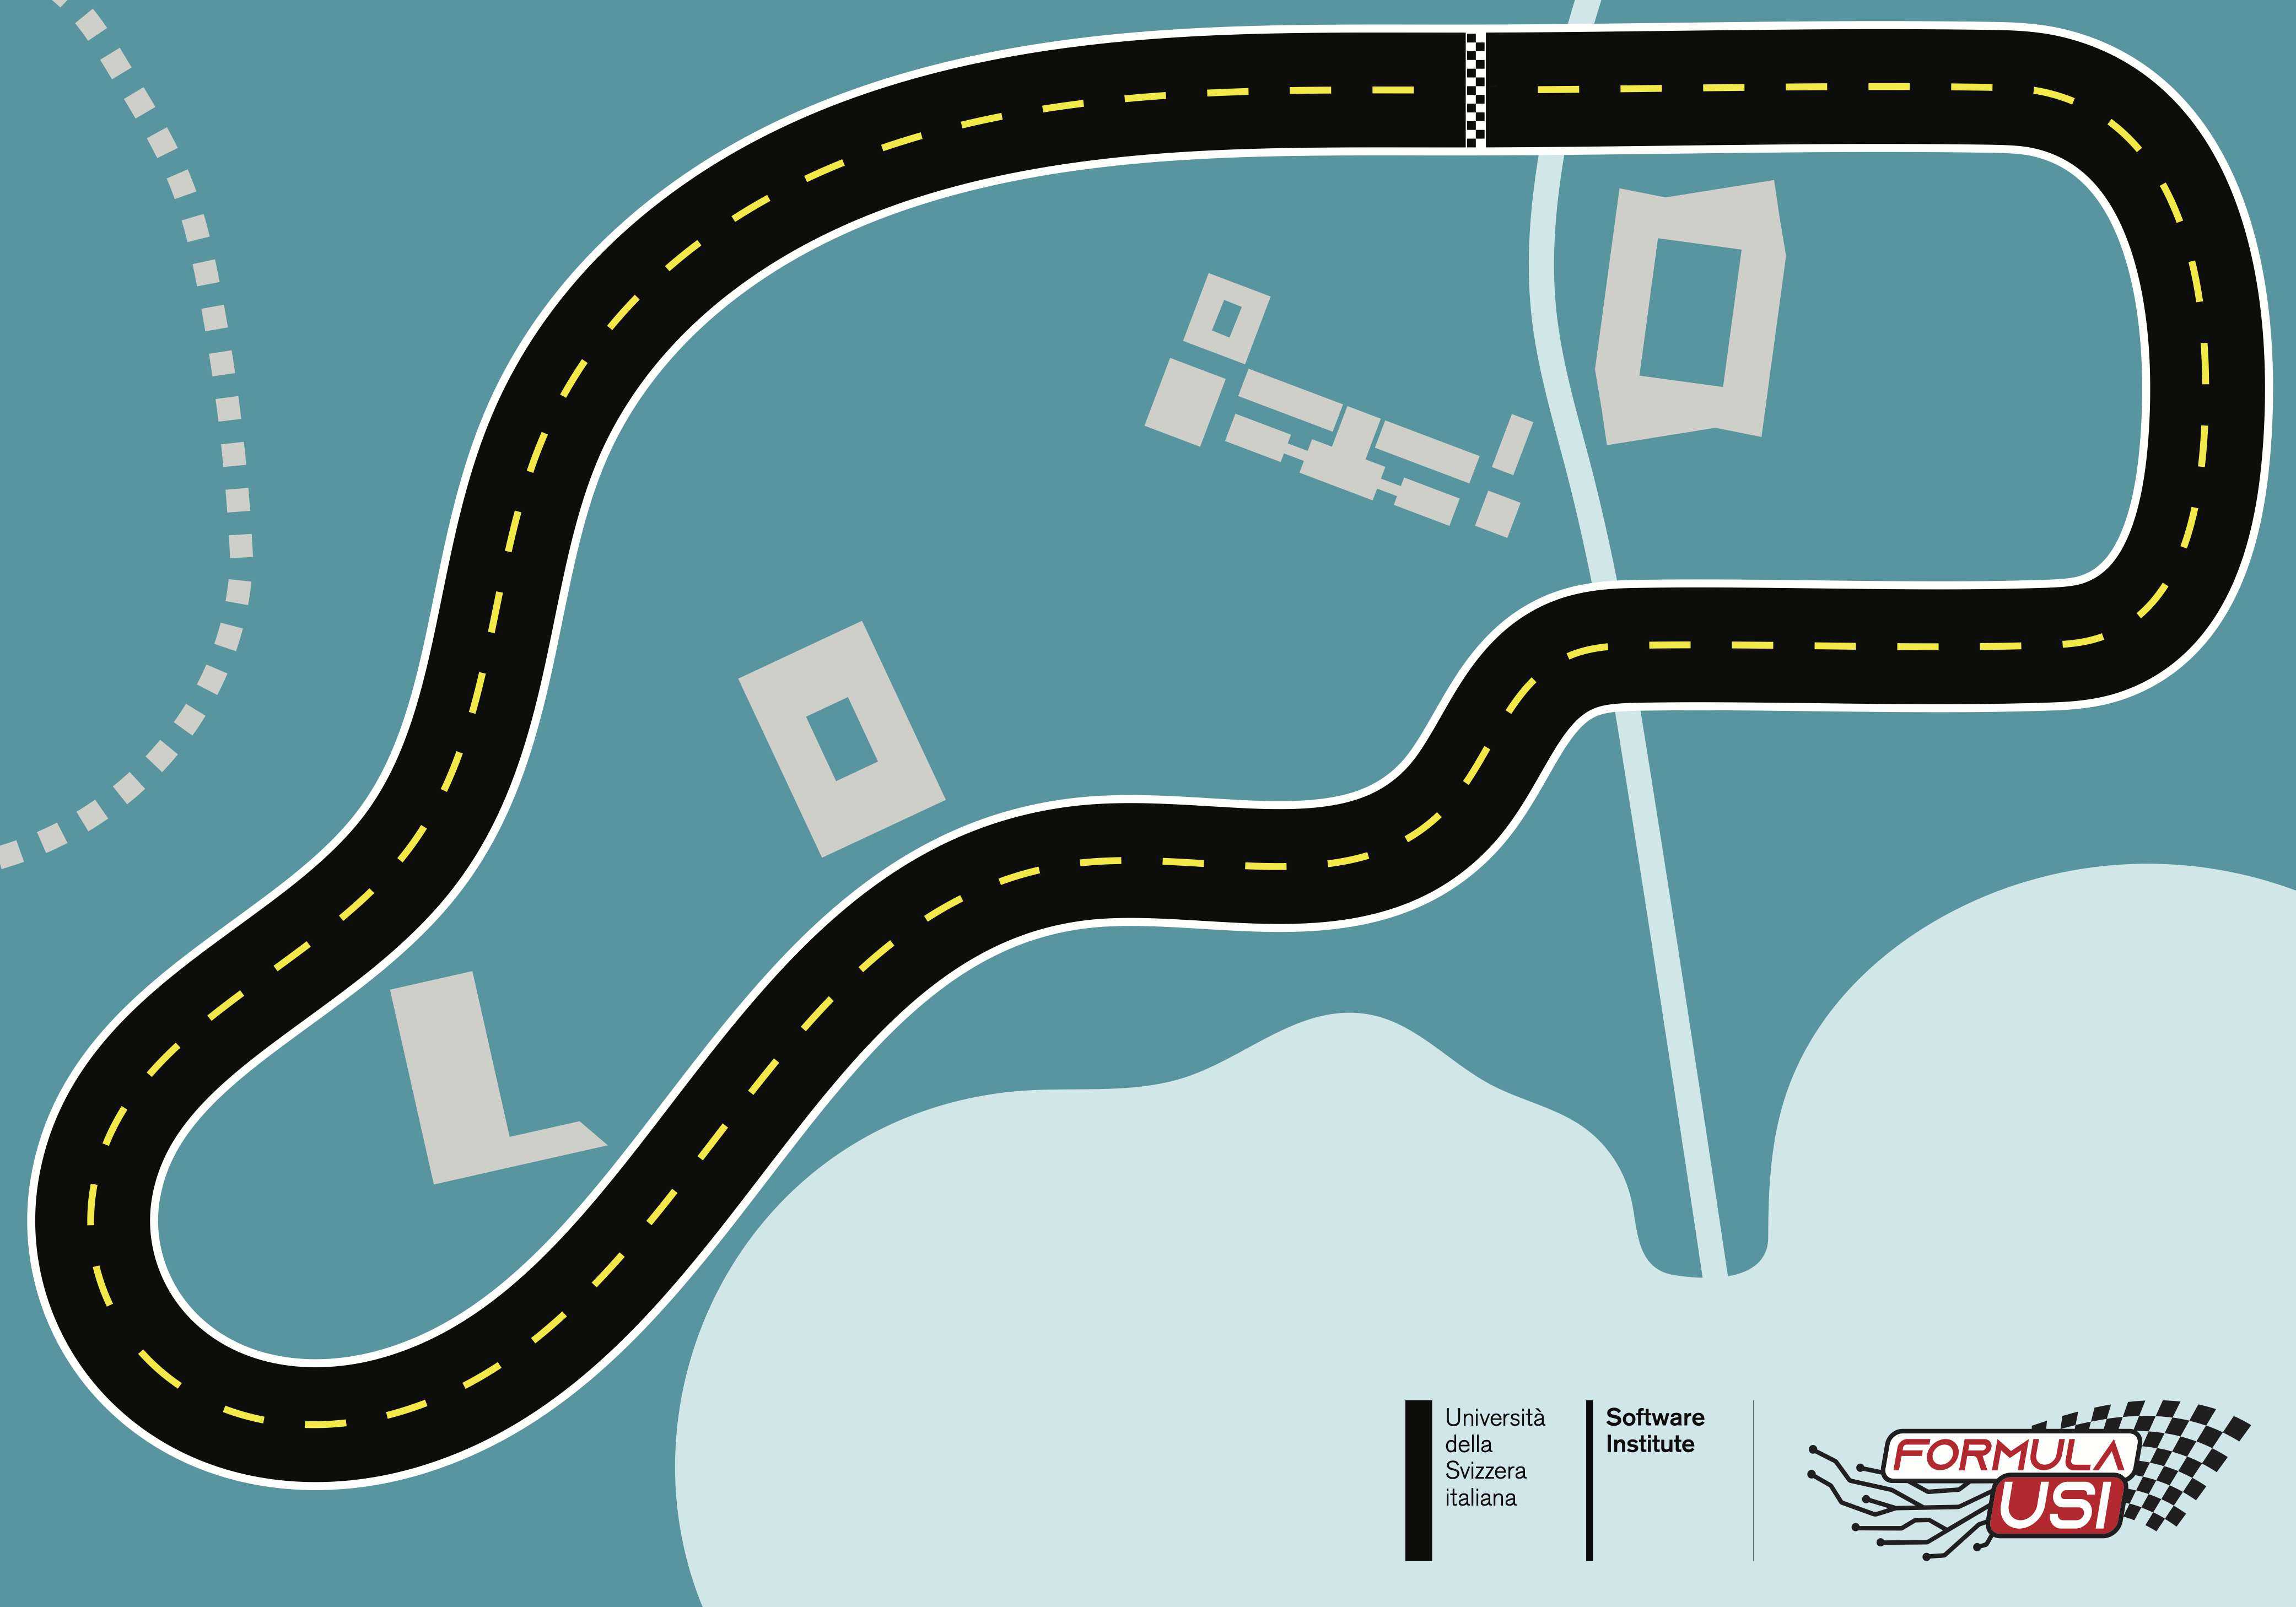
\includegraphics[width=.98\textwidth]{setup/usi_track_real.png}
		\captionof{figure}{Real track}
		\label{fig:usitrack}
	\end{minipage}%
	\begin{minipage}{.5\textwidth}
		\centering
		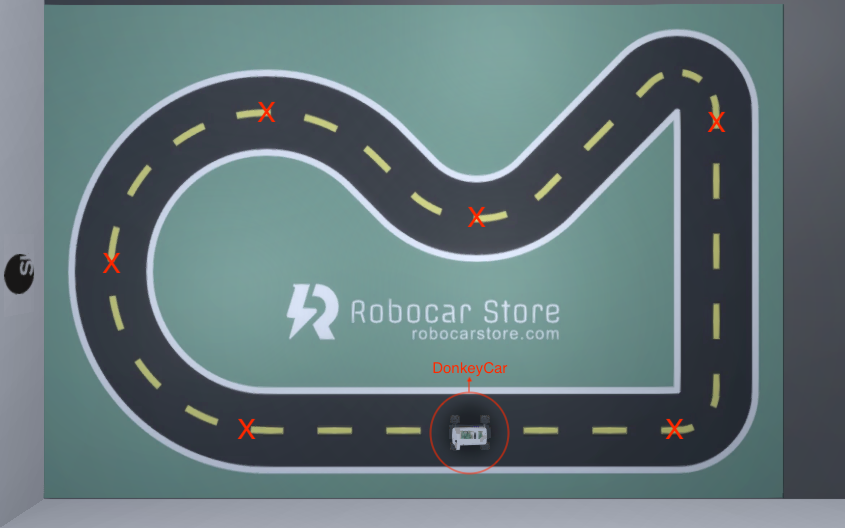
\includegraphics[width=.94\textwidth]{setup/usi_track.png}
		\captionof{figure}{Simulated track}
		\label{fig:usitracksim}
	\end{minipage}
\end{figure}

For our experiments in the simulated environment, we used the virtual replica of such track, which was created in Unity~\footnote{https://www.unity.com} by a previous thesis in the lab. Additionally, we added a starting line in the simulated track in order to record the number of times the car completes a lap. Such information is important to understand the progress of the RL agent during training. Both tracks are single-lane since the DonkeyCar occupies 50\% of the track when it is placed in the middle of the yellow dashed line. However, the track is an interesting testbed for RL and self-driving in general since it has a mixture of sectors that are easy to drive and curves that are challenging to take.

Regarding the Gym environment, we built upon the codebase of ~\cite{learning-to-drive-in-5-minutes}. Specifically, the \textit{observation space} of both the real and simulated agent consists of RGB images of size $320 \times 240$ collected at 20\textit{Hz} (i.e. 20 frames per second). 

The \textit{action space} is composed of two continuous actions, i.e. steering and throttle, both varying in the interval $[-1, 1]$. Indeed, the action space must be symmetric since most RL algorithms use a Gaussian distribution (with mean 0 and standard deviation of 1) for exploration of continuous action spaces and a non-symmetric action space would harm learning~\footnote{https://stable-baselines.readthedocs.io}. Consequently, the throttle is rescaled to take values in the interval $[0, 1]$. However, for simplicity and for speeding up learning especially in the real world, we kept the throttle constant throughout training. Furthermore, In order to obtain a smooth control of the car, the change in steering angle is \textit{constrained} by keeping a history of steering angles at previous time steps. This ensures that the difference between steering angles in two consecutive time steps stays within a given range~\cite{learning-to-drive-in-5-minutes}.

Since we use an encoder to represent the images in a lower dimension, we used a custom Gym wrapper to convert the raw images coming from the simulator or the real world into the corresponding latent space. Moreover, we stack four consecutive frames, i.e. converted into the corresponding latent space representations, such that the agent can perceive the motion of the car by taking an action every four frames~\cite{dqn}.

Regarding the \textit{reset} of the environment we used two different modalities in simulation and in the real world. In simulation, the DonkeyCar simulator provides the \textit{cross track error} (XTE) measurement, which is defined as the distance between the center of the mass of the car and the center of the lane. Such metric varies in the interval $[-2, 2]$ when the car is \textit{fully} on-track, i.e. its center of mass is in the middle of either white lines; therefore, when the absolute value of the XTE is outside of such interval the car can be considered off-track. In particular, we used the boundary value of $3$, which corresponds to having the car with all four wheels off-track; in such case the episode terminates unsuccessfully. On the other hand, in the real world the XTE is not available. Therefore, we resort to a manual stopping strategy to terminate the episode, by remotely signaling the agent to stop controlling the car.

Finally, in real world, we established a success criterion to deem a certain episode successful. In particular, we chose to stop an episode when the number of timesteps reach the threshold level of 1000. Such threshold corresponds to approximately two laps around the track or alternatively 50 seconds given that the frame rate is 20\textit{Hz}. Indeed, the number of laps carried out by a trained RL agent depends on how \textit{smooth} is the control, since steering actually slows down the car. In simulation, instead, such criterion is set to a completed a lap, and also in this case the number of steps carried out in a lap may vary based on the smoothness of the motion. However, the limit of 1000 steps is kept also in simulation.

%\section{The track and the environment} \label{sec:track}
%The track we used is called USI track, shown in Figure \ref{fig:usitrack}. It strongly resembles one used by \citet{DBLP:journals/corr/abs-2008-00715} in Learning to Drive. We do have a simulated version built in Unity and an actual printed track. The choice fell on this track since it is complete, it includes a straightaway, right turn, left turn, wide turn and very steep turn. Beside that, \citet{DBLP:journals/corr/abs-2008-00715} already proved that the agent can learn on this type of track and the focus of this thesis is more on replicating a real agent learning to self-drive in real world and not creating a new model with a particular feature.
%
%\begin{figure}[h]
%    \centering
%\begin{minipage}{.5\textwidth}
%    \centering
%    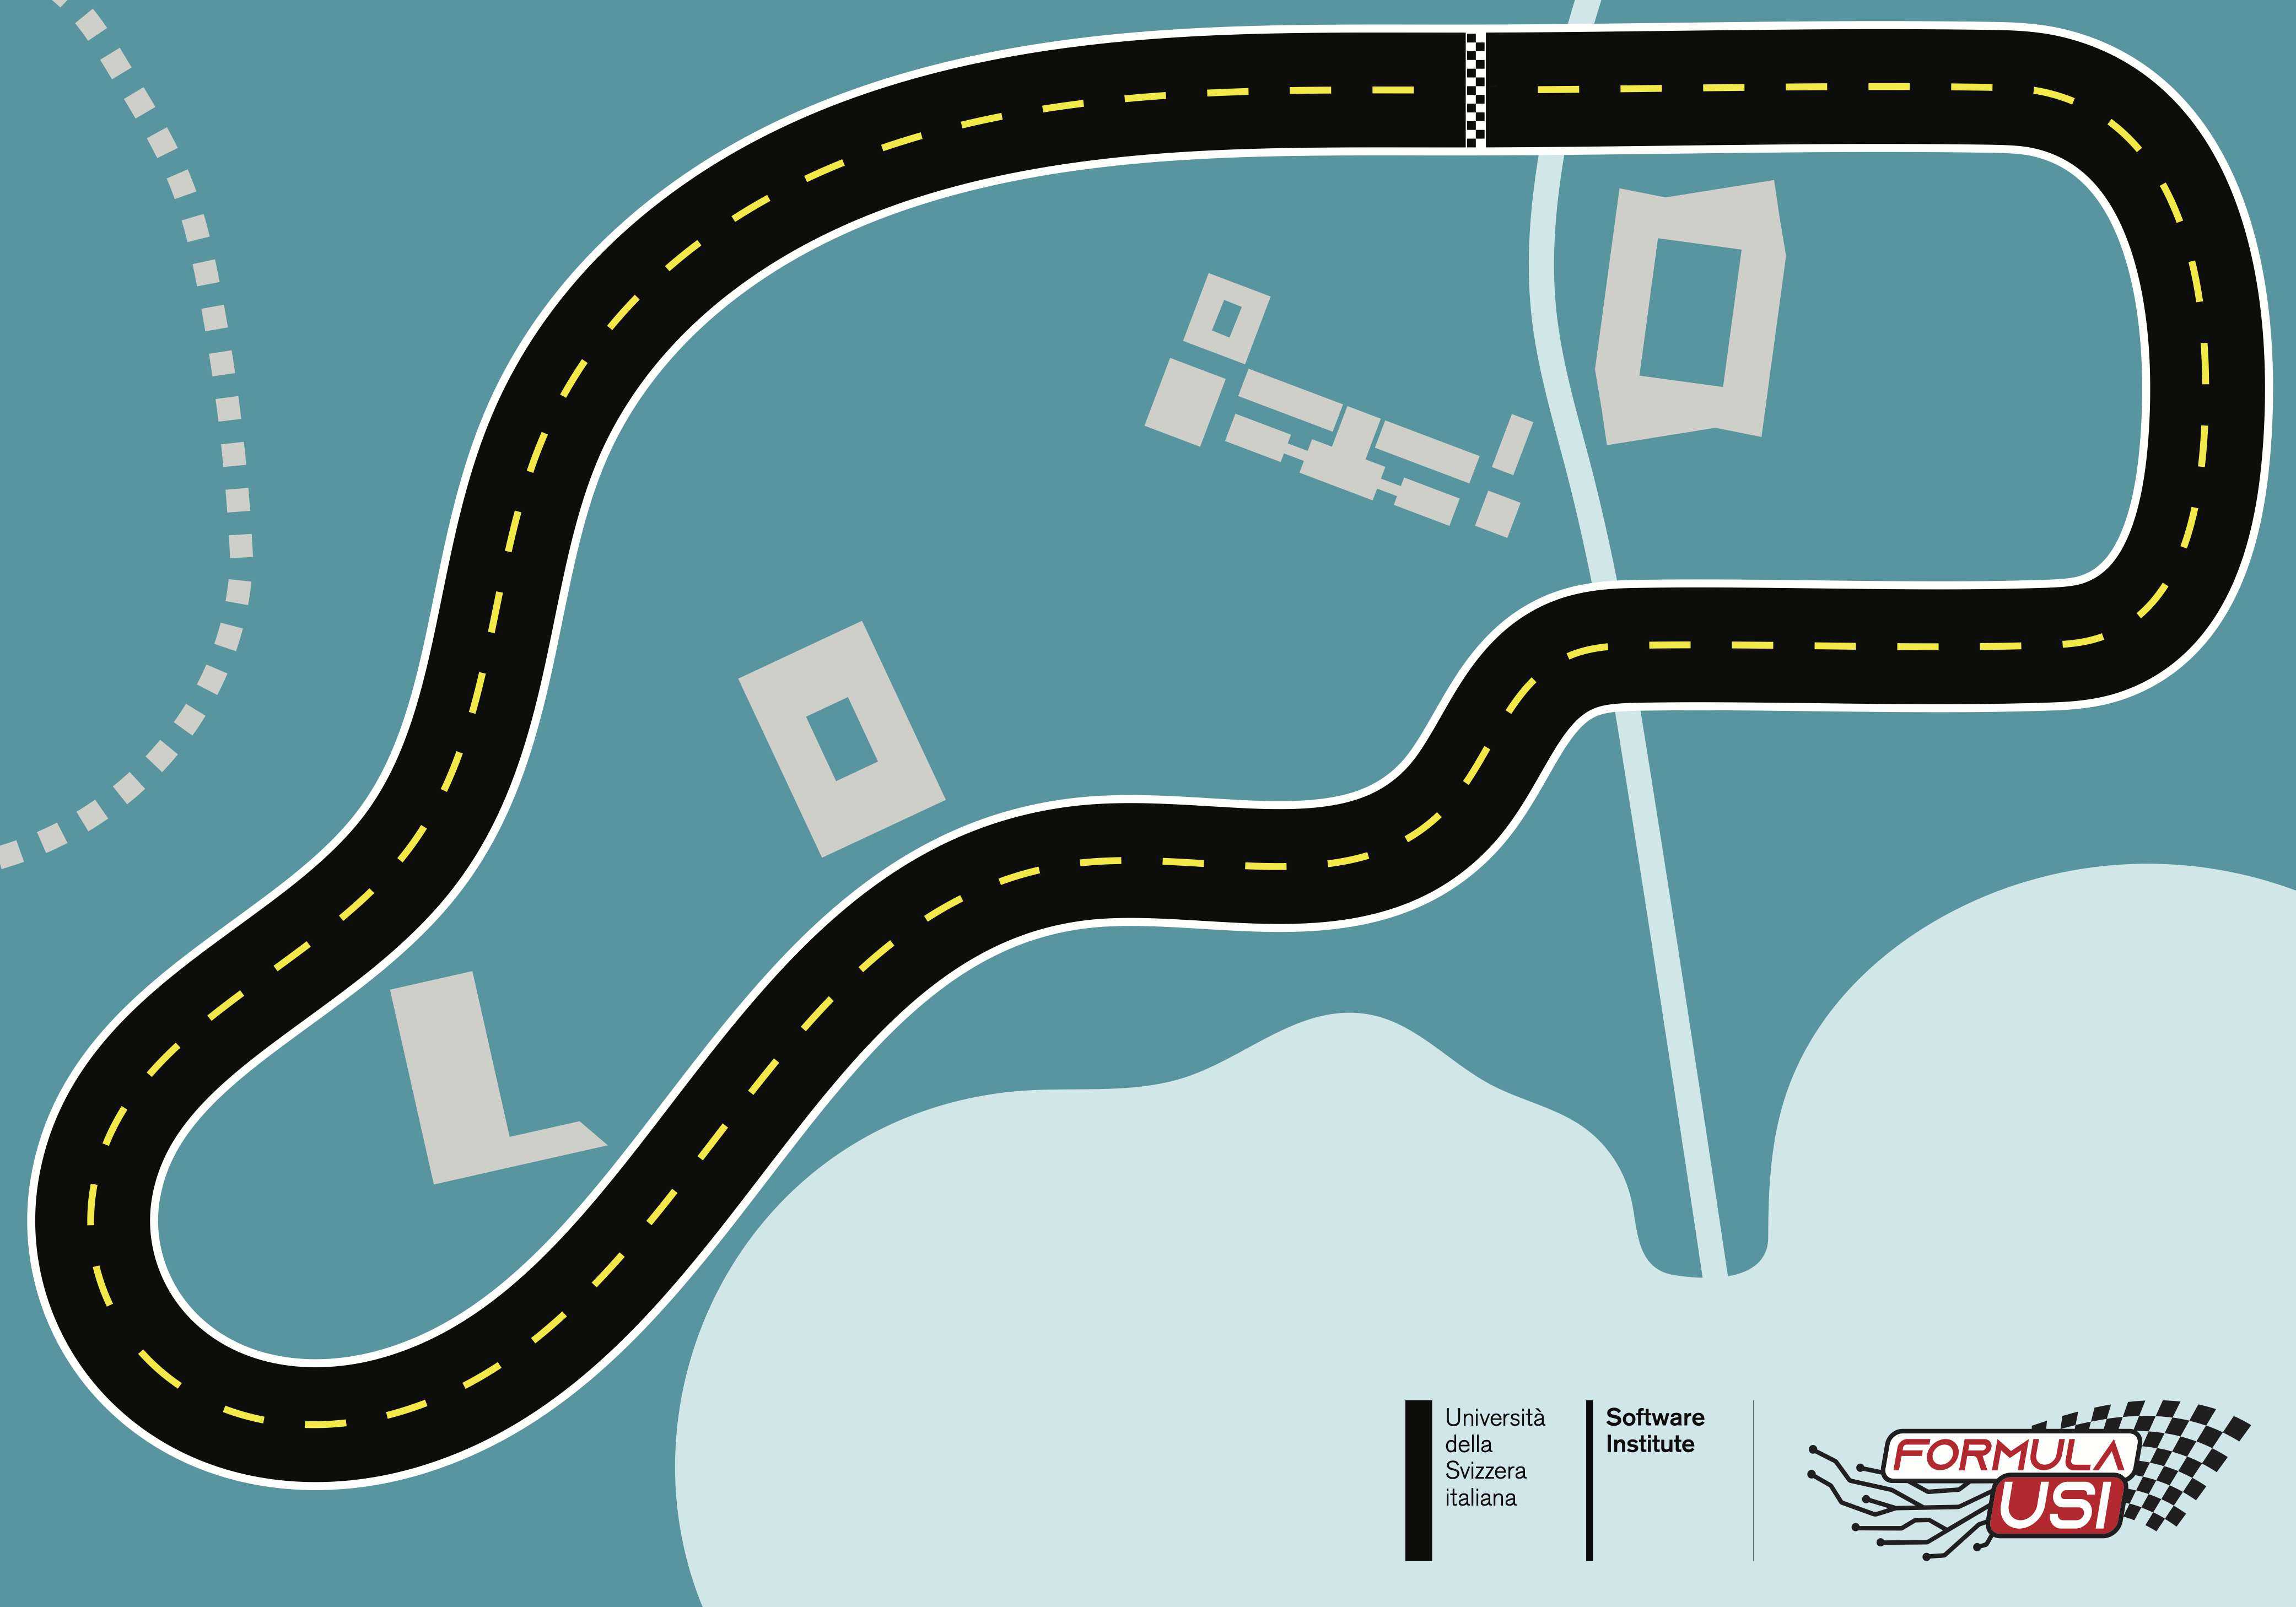
\includegraphics[width=0.85\textwidth]{setup/usi_track_real.png}
%    \captionof{figure}{Real USI track TODO}
%    \label{fig:usitrack}
%\end{minipage}%
%\begin{minipage}{.5\textwidth}
%    \centering
%    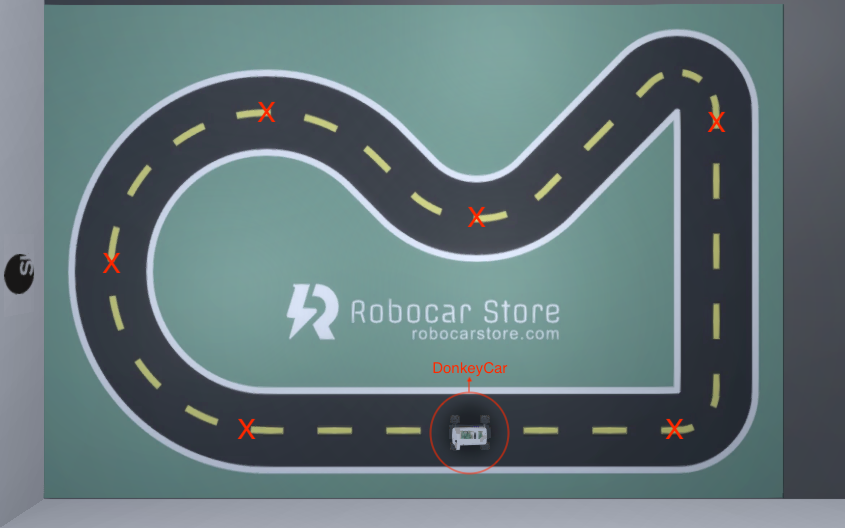
\includegraphics[width=0.95\textwidth]{setup/usi_track.png}
%    \captionof{figure}{Simulated USI track}
%    \label{fig:usitracksim}
%\end{minipage}
%\end{figure}
%
%The learning of the agent, as shown later on, is straightforward, except the very steep turn which is considerably harder than the others. This difficulty is due to the limited steering angle of the robot and in the real world the aforementioned adversity is even more marked as well see. 
%
%The default starting line in both tracks is where the Donkey is placed in Figure \ref{fig:usitracksim}. Certainly, in the real track it is an imaginary line that we use as a starting point and of course the laying of the car at each episode beginning cannot be exact but approximate. Beside that, there are a few checkpoints, approximately highlighted with a cross in Figure \ref{fig:usitracksim}, troughout the track that can be used as starting points depending on the learning strategy chosen. The simulator provides the following possibilities:
%
%\begin{itemize}
%    \item \textbf{Start:} The episode start always at the starting line.
%    \item \textbf{Checkpoint:} The episode start at the latest checkpoint reached during the previous episode.
%    \item \textbf{All:} All the checkpoints are used cyclically starting from the starting line and proceeding one by one forward for each episode.
%    \item \textbf{Random: } The starting point is chosen randomly, between the available checkpoints, at the beginning of each episode.
%\end{itemize}
%Furthermore, the simulator let us choose where a lap ends. It can end where the DonkeyCar started or at the starting line.

%TODO: AGGIUNGI referenza punti di partenza.

%\section{DonkeyCar}
%
%The real Remote Controlled DonkeyCar is essentially a standard DonkeyCar as described in Section \label{sec:donkeycar}. To recap it is a remote controlled car equipped with a microcontroller NVIDIA Netson Nano and a camera sensor. The RGB pictures are taken at a resolution of $320x240$ and at $20hz$ (20 frames per second), which means the algorithm must finish all iteration steps within $0,05$ seconds otherwise it would skip some frames and the learning or the driving may be compromised by the agent's non-responsiveness. This limitation is present only in real world since the simulator time can be slowed down to meet the needs. In our setting we have a standard 3 cell LiPO battery of 11.1V and 2200 mAh to power just the motors and the controller. During the training in the real world we often noticed a slow regression in term of speeds of the car, iteration after iteration. However, this problem can be solved by disconnecting the LiPO battery for a moment from time to time to restore full speed, which is why we suspect this problem may be caused by the battery. Furthermore, an external power bank with 10000mAh/37Wh of capacity and an output of 5V and 2.4A powers the Jetson Nano which with this capacity, is more than enough to overcome the longevity of the LiPO battery.

\section{Dataset}
In order to train the encoders for the simulated and the real world, we collected two different datasets by driving the car in the respective environment. Examples of collected images are respectively shown in Figure~\ref{fig:datasetsim} and in Figure~\ref{fig:datasetreal}.

\begin{figure}[h]
	\begin{minipage}{.33\textwidth}
		\centering
		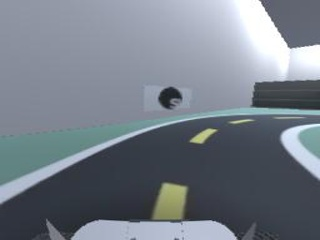
\includegraphics[width=0.95\textwidth]{setup/s1.jpg}
	\end{minipage}%
	\begin{minipage}{.33\textwidth}
		\centering
		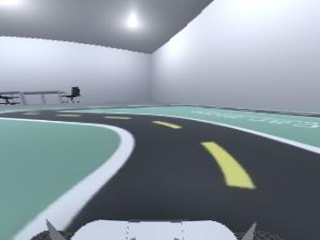
\includegraphics[width=0.95\textwidth]{setup/s2.jpg}
	\end{minipage}%
	\begin{minipage}{.33\textwidth}
		\centering
		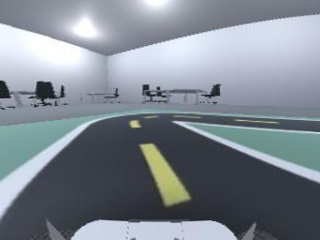
\includegraphics[width=0.95\textwidth]{setup/s3.jpg}
	\end{minipage}
	\captionof{figure}{Images extracted from the simulated dataset}
	\label{fig:datasetsim}
\end{figure}

\begin{figure}[h]
	\begin{minipage}{.33\textwidth}
		\centering
		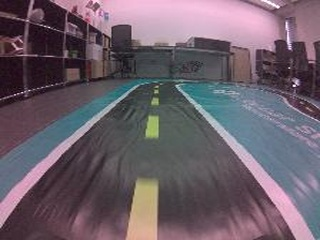
\includegraphics[width=0.95\textwidth]{setup/r1.jpg}
	\end{minipage}%
	\begin{minipage}{.33\textwidth}
		\centering
		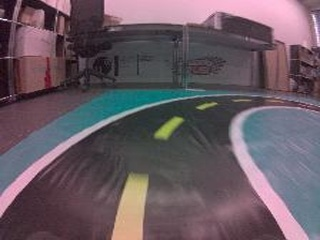
\includegraphics[width=0.95\textwidth]{setup/r2.jpg}
	\end{minipage}%
	\begin{minipage}{.33\textwidth}
		\centering
		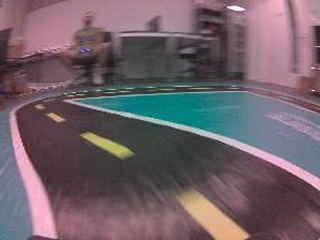
\includegraphics[width=0.95\textwidth]{setup/r3.jpg}
	\end{minipage}
	\captionof{figure}{Images extracted from the real dataset}
	\label{fig:datasetreal}
\end{figure}

In both environments we collected a dataset of $\approx$ 10\textit{k} images which correspond to $\approx$ 10 minutes of driving at $20$\textit{Hz}. We payed extra care when collecting the images in the real world by ensuring that the lighting conditions were consistent in all images; such conditions were also kept during training of the RL agent. Collecting the dataset for training the encoders does not require a good quality of driving, since labels are not recorded. However, it is important to capture all the sectors of the track such that the RL agent can extensively explore the track during training and always have a good representation of the observation it will encounter. Indeed, the pretrained encoder will not be updated during the online training of the agent.

%During the experiments resulted that a dateset of $\sim 10000$ pictures was enough to reach our goals, furthermore notice that smaller datasets may not be sufficient for the encoder to learn a good representation. To collect each of the datasets are enough $\sim10$ minutes if we run the algorithm at $20hz$ (20 frames per second) as we did. Beside that, all the pictures from the real world must be collected with a certain environmental condition that should remain consistent in time, also during the training of the agent to avoid problems. In our case, it was collected with all windows closed and the with maximum light to make it easy to be replicated. 

Before the pretraining phase of the encoder we applied a preprocessing phase of the images. In particular, we cropped the top 80 pixels from each image and resized it to $160 \times 80$. Cropping is useful to remove the part of the image that is not relevant to driving, while downscaling the image has the advantage of saving computation time when training the encoder. Figure~\ref{fig:datasetsimcropped} and Figure~\ref{fig:datasetrealcropped} show samples of cropped and resized images that are passed as input to the encoder during training. As we can see, resizing down to $160 \times 80$ does not degrade significantly the quality of the images. Moreover, the real images look like they have undergone more cropping than their simulated counterpart. The reason is that the position of the camera of the car is slightly different between simulation and real. Indeed, the \textit{simulated camera} is tilted upwards w.r.t. \textit{real camera} and this gives the impression that in the real images more pixels have been cropped.

%Since we want our RL agent to focus exclusively on the track we found convinient to crop the top 100 rows of each pictures to remove the background, and to reduce the complexity of our algorithm, we downscale each images from $320x140$ to $160x80$ before feeding them to the encoder. The resulting pictures are shown in Figures \ref{fig:datasetsimcropped} and \ref{fig:datasetrealcropped}. Note that during training, the training set is split in validation and training set with a ratio $20/80$ and the test set is collected apart and consist of $\sim 1000$ images for each dataset.

\begin{figure}[h]
	\begin{minipage}{.33\textwidth}
		\centering
		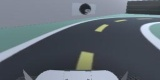
\includegraphics[width=0.95\textwidth]{setup/cs1.jpg}
	\end{minipage}%
	\begin{minipage}{.33\textwidth}
		\centering
		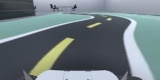
\includegraphics[width=0.95\textwidth]{setup/cs2.jpg}
	\end{minipage}%
	\begin{minipage}{.33\textwidth}
		\centering
		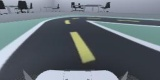
\includegraphics[width=0.95\textwidth]{setup/cs3.jpg}
	\end{minipage}
	\captionof{figure}{Examples of cropped simulated images}
	\label{fig:datasetsimcropped}
\end{figure}

\begin{figure}[h]
	\begin{minipage}{.33\textwidth}
		\centering
		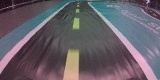
\includegraphics[width=0.95\textwidth]{setup/cr1.jpg}
	\end{minipage}%
	\begin{minipage}{.33\textwidth}
		\centering
		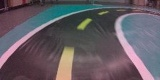
\includegraphics[width=0.95\textwidth]{setup/cr2.jpg}
	\end{minipage}%
	\begin{minipage}{.33\textwidth}
		\centering
		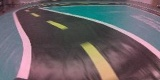
\includegraphics[width=0.95\textwidth]{setup/cr3.jpg}
	\end{minipage}
	\captionof{figure}{Examples of cropped real images}
	\label{fig:datasetrealcropped}
\end{figure}

Finally such images collected in the simulator and in the real world are also useful for training the CycleGAN architecture~\cite{CycleGAN2017}. In order to save computation time the dataset we provided to the CycleGAN training process is smaller, i.e. $\approx$ 5\textit{k} images for each domain, i.e. simulated and real, since previous work shows that such size is adequate to represent the track we are considering~\cite{stocco-mind}.

%Finally, for the cyclegan, the dataset can be even smaller $\sim 5000$ pictures for both real and simulation. No crop is applied and a resize to $256x256$ pixels is done to match the network size provided by \citet{CycleGAN2017}. And the test sets match the ones used for the encoders. After applying the cyclegan in our experiments, the pictures are reshaped and cropped to match the need of the autoencoder.

\section{Training}

To train the RL agent we adopted the SAC algorithm due to its sample efficiency and the ability to reuse the collected experience~\cite{art:sac}. Such abilities are paramount when training an agent in the real world. We used the hyperparameters provided by \cite{learning-to-drive-in-5-minutes} for the task of driving. In particular, we chose a replay buffer of size $300$\textit{k} (i.e. the number of transitions that can be stored) and a multilayer perceptron with two layers of 64 units each both for the actor and the critic. Moreover, training is carried out at the end of each episode for 64 gradient steps. Thanks to the dimensionality reduction step, the transitions in the replay buffer contain latent vectors rather than entire images; as a consequence training is relatively fast and it can be carried out in machine without GPU. 

%\subsection{Simulation}\label{subsec:sim}
In simulation, the training is performed using a client-server architecture where both client and server run on the same machine. The server, i.e. the Donkey simulator, provides the frames captured by the simulated camera at each timestep together with the \textit{telemetry} of the car, i.e. its position, velocity and XTE. The client, i.e. the learning component, receives the frames and the telemetry and it is tasked to make a control decision, i.e. it has to return to the server the action to undertake on the car. Once the server receives the action, the simulator applies it on the car and the cycle continues. The decision to start or stop an episode is delegated to the client, which according to the telemetry received by the simulator at each step, decides when to reset the environment. When an episode terminates, the training procedure starts. Afterwards the simulation is stopped for the entire duration of training and it is resumed as soon as the training finishes.

%\begin{wrapfigure}{r}{0.6\textwidth}
\begin{figure}[h]
	\begin{center}
		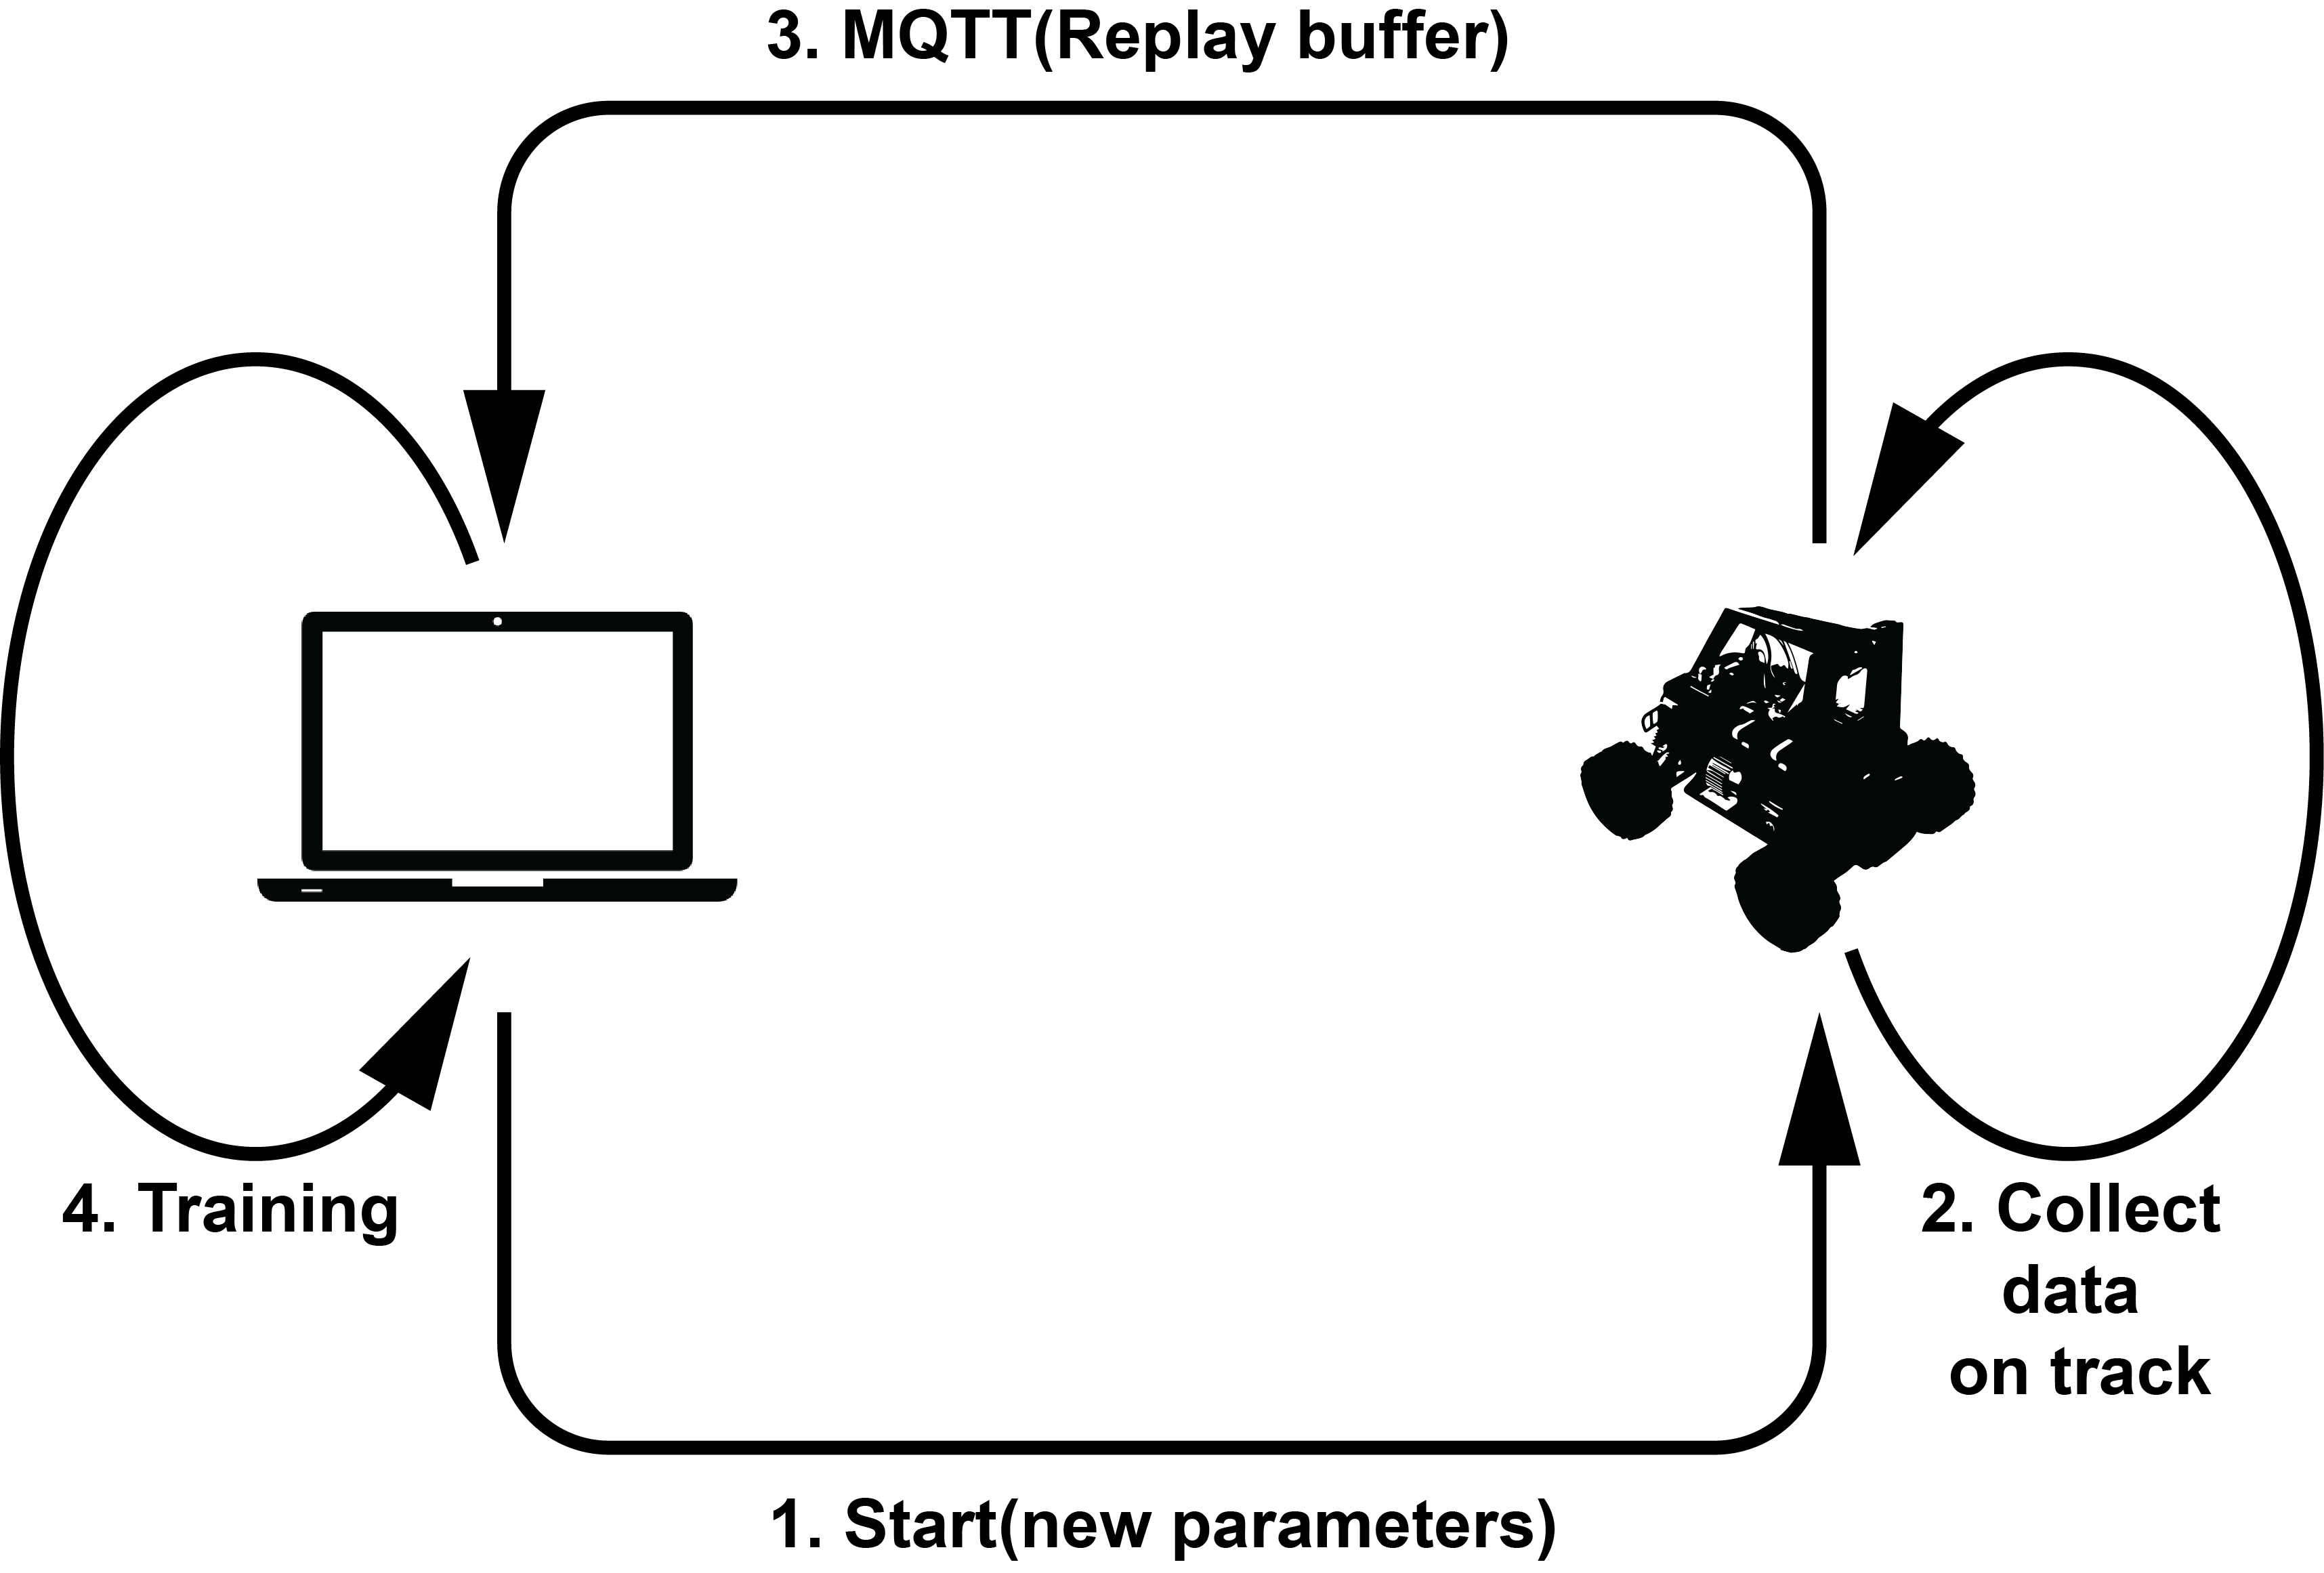
\includegraphics[width=0.60\textwidth]{setup/comm.png}
	\end{center}
	\caption{Key steps in the real training procedures}
	\label{fig:comunication}
\end{figure}
%\end{wrapfigure}

Also In the real environment we used a client-server architecture for training. However, client and server run on different machines, as shown in Figure~\ref{fig:comunication}. This is because the Donkey microcontroller has limited computation capabilities and, most importantly, a limited battery. Indeed, carrying out the RL agent training on the Donkey would quickly deplete the battery and slow down training due to frequent battery recharge and replacement. Moreover, having two dedicated machines also allows a human operator to remotely stop an episode, appropriately reset the car to its initial position and remotely restart it.

In particular, we used the MQ Telemetry Transport (MQTT) messaging protocol, which is one of the most used in the internet of things domain. The protocol defines all the rules that determine how devices exchange messages over the internet, i.b. by writing (publish) and reading (subscribe) data. The sender (publisher) and the receiver (subscriber) communicate on message channels called \textit{topics} and are decoupled from each other. The protocol also involves the presence of a \textit{broker} that has access to the incoming messages and distributes them correctly to the subscribers of a certain topic. Specifically, we used the \textit{HiveMQ} broker which allows the connection of up to 100 clients free of charge. The topics defined to manage the communication between the DonkeyCar and the client machine are as follows:

\begin{itemize}
    \item \textbf{Stop car:}. (Client - Publisher, Donkey - Subscriber). When the client machine publishes a message on this topic the RL agent on the Donkey stops controlling the car, i.e. the episode must terminate. Practically the human operator presses the space bar on the keyboard which triggers the signal;
    \item \textbf{Replay buffer:} (Donkey - Publisher, Client - Subscriber). Once an episode terminates, the Donkey publishes on this topic all the transitions collected during the episode. The client machine receives such transitions and stores them in the replay buffer which is used to train the policy. The transitions only contain the latent space representations of the captured images in the real world; indeed, the encoder runs on the Donkey and transforms each frame into its corresponding latent space representation in order to be processed by the policy. This way the transitions exchange is quicker than sending raw images;
    \item \textbf{Replay buffer received:} (Client - Publisher, Donkey - Subscriber). The client uses this topic to acknowledge the Donkey that it has received the transitions. This topic is useful when the replay buffer of the episode gets longer, hence the Donkey sends the data in chunks and before sending the next chunk it needs to know that the client has finished reading the previous in order to avoid overlapping. 
    \item \textbf{Parameters:} (Client - Publisher, Donkey - Subscriber). The client has a copy of the parameters of the policy used by the Donkey. Once the client receives the transitions the training starts. During training the human operator can retrieve the car and position it back on track. Once the training is complete, the client machine publishes the updated policy parameters and the Donkey updates its copy of the policy parameters;
    \item \textbf{Start episode:} (Client - Publisher, Donkey - Subscriber). The client uses this topic to acknowledge the Donkey that a new episode must start. Practically the human operator presses the enter key on the keyboard which triggers the signal;
\end{itemize}
%\section{Communication - MQTT}
%
%As described in Section \ref{subsec:real}, when training in real world, the host machine and the DonkeyCar must communicate wirelessly multiple times during the training. MQ Telemetry Transport (MQTT) is the most used messaging protocol for the Internet of Things (IoT). It includes all the rules that define how devices can write (publish) and read (subscribe) data over the internet. The sender (Publisher) and the receiver (Subscriber) communicate via topic and are decoupled from each other. The connection between them is handled by an MQTT broker that filters all incoming messages and distributes them correctly to the Subscribers of the topic. In pratice any device can publish a message on a topic, then the broker take care of dispatching it to subscribers of that topic. In particular we used the HiveMQ broker that allows the connection of up to 100 clients with no cost. The topics defined to manage the communication between the host machine and the DonkeyCar are:
%
%\begin{itemize}
%    \item \textbf{Stop car:} The host machine writes a signal on this topic, that is constantly monitorated by the DonkeyCar, to inform that the episode must terminate.
%    \item \textbf{Replay buffer:} Once the episode terminate, all the collected information by the DonkeyCar are sent to the host machine through this topic.
%    \item \textbf{Replay buffer received:} The host machine uses this topic to acknowledge DonkeyCar that it has received the buffer.
%    \item \textbf{Parameters:} Once the training is complete, the host machine sent the updated neural network parameters through this topic.
%    \item \textbf{Start episode:} The host machine uses this topic to acknowledge DonkeyCar that a new episode can start.
%    \item \textbf{Speed modifier:} This topic can be used by the host machine to inform the DonkeyCar that it must change its throttle by the sent value that can be either positive or negative.
%\end{itemize}


%\section{Training modality}
%
%\subsection{Simulation}\label{subsec:sim}
%In simulation, the training of the agent is straightforward since all the operation are done on the host machine, moreover it is not required a GPU machine to accomplish all the steps in time, at least until the cyclegan is introduced. Even though an on-policy RL algorithm could be implemented, an off-policy algorithm is chosen since in real world, in our setting, the on-policy method is not replicable given the limited computational power of the microcontroller. Beside that, we want to compare the same type of algorithm in the two type of environments. In pratice, a pretrained AE/VAE provides a representation of the state in the form of a latent vector, the agent drives with a policy kept constant during the episode and all the frames and actions are collected into a buffer. When the simulator reports that the car has crashed or went out of track more than a predefined distance, the episode terminates. The episode ends also when the car has reached the starting point or, in our setup, it reaches 1000 steps. Finally, at the end of the episode, a policy is trained using the collected buffer and the new parameters are used to update the driving policy.
%
%\subsection{Real world} \label{subsec:real}
%Since the microcontroller equipped by the DonkeyCar is a low capability calculator, a few precautions need to be taken in order to to train the agent. Firstly, as mentioned above, an off-policy method like SAC allows to relocate the actual training, and consequently the very expensive gradient back-propagation, to another machine with more resources. Secondly, the use of representation learning (AE/VAE) allows to reduce significantly the size of the RL neural networks and moreover the pre-training of the encoder can be done in advance on the host machine speeding up the process. In practice the functioning is similar to the one seen in previous Section \ref{subsec:sim}. The microcontroller operates the driving policy, collect the image, forward it through the AE/VAE, then the agent chose an action based on that representation. This process is repated until a human supervisor ends the episode for the car gone off the track. The episode also terminates when the DonkeyCar reaches, in our setup, 1000 steps. Hereafter, all the steps information, like latents vectors, actions and rewards are collected into a buffer up to a predefined size and are sent through the network to the host calculator that actually train the policy at the end of the episode. After the training, the new parameters are sent back to the DonkeyCar and the process is repeated until convergence.
%
%\section{Communication - MQTT}
%
%As described in Section \ref{subsec:real}, when training in real world, the host machine and the DonkeyCar must communicate wirelessly multiple times during the training. MQ Telemetry Transport (MQTT) is the most used messaging protocol for the Internet of Things (IoT). It includes all the rules that define how devices can write (publish) and read (subscribe) data over the internet. The sender (Publisher) and the receiver (Subscriber) communicate via topic and are decoupled from each other. The connection between them is handled by an MQTT broker that filters all incoming messages and distributes them correctly to the Subscribers of the topic. In pratice any device can publish a message on a topic, then the broker take care of dispatching it to subscribers of that topic. In particular we used the HiveMQ broker that allows the connection of up to 100 clients with no cost. The topics defined to manage the communication between the host machine and the DonkeyCar are:
%
%\begin{itemize}
%    \item \textbf{Stop car:} The host machine writes a signal on this topic, that is constantly monitorated by the DonkeyCar, to inform that the episode must terminate.
%    \item \textbf{Replay buffer:} Once the episode terminate, all the collected information by the DonkeyCar are sent to the host machine through this topic.
%    \item \textbf{Replay buffer received:} The host machine uses this topic to acknowledge DonkeyCar that it has received the buffer.
%    \item \textbf{Parameters:} Once the training is complete, the host machine sent the updated neural network parameters through this topic.
%    \item \textbf{Start episode:} The host machine uses this topic to acknowledge DonkeyCar that a new episode can start.
%    \item \textbf{Speed modifier:} This topic can be used by the host machine to inform the DonkeyCar that it must change its throttle by the sent value that can be either positive or negative.
%\end{itemize}
%
%Notice that this protocol is not complety reliable so some precautions and check must be done when implenting it, especially in real-time system where some actions cannot be delayed.
\chapter{Experiments}

\section{Representation Learning: AE vs VAE}

As described in previous sections, we use want to use state representation learning techniques to decouple state learning from policy learning, as previous works show that it considerably speeds up the training process~\cite{DBLP:journals/corr/abs-2008-00715,DBLP:journals/corr/abs-1910-01741}. We evaluate two strategies, i.e. an AutoEncoder and a Variational AutoEncoder, to understand if the stochasticity of VAEs can help in learning a good representation of the actual state. 

In order to chose which representation learning strategy to use, we train AE and VAE with the same architecture, i.e., with an encoder composed of three  convolutional layers interposed by ReLU functions and a variable size output layer; similarly the decoder is composed of three deconvolutional layers and the output layer is a sigmod. The detailed architecture can be found in Appendix~\ref{app:ae/vae}. Both AE and VAE have been trained for 50 epochs with an early stopping after five epochs of no improvement of the validation loss.

The latent space size ($z$) must be carefully chosen such that the latent space is able to represent all the features of the images and consequently produce high quality reconstructions. The latent space size, also determines the size of the states in the replay buffer transitions and, consequently, the training speed. In particular, we consider latent vectors of size 32 and 64.

We also investigated whether adding augmentation during training has an impact on the learned representations. In particular, we consider several augmentation methods such as Gaussian and motion blurring, contrast normalization, additive Gaussian noise, sharpening and coarse dropout. During training each operation can be applied with a certain probability and the sequence of operations is randomized.

For every combination of training set (simulated/real), representation strategy (AE/VAE), latent space size (32/64) and augmentation (True/False), we train the corresponding architecture three times. Each model is evaluated on the corresponding test set (i.e. simulated or real) and the resulting average reconstruction loss is averaged across the three training repetitions.

\begin{table}[h]
	\centering
	\begin{tabular}{|c|c||c|c|c|c|}
		\hline
		Z & AUGMENTATION & MEAN & STD & MAX & MIN \\ \hline
		\multirow{2}{*}{32} & False & 121.54 & 102.42 & 795.44 & 45.61 \\
		& True & 164.57 & 95.51 & 783.03 & 65.13  \\ \hline
		\multirow{2}{*}{64} & False & \textbf{103.54} & 79.14 & 588.14 & 40.84 \\
		& True & 137.24 & 74,02 & 611,81 & 63,05  \\ \hline
	\end{tabular}
	\caption{AE trained in simulation - reconstruction loss}
	\label{tab:aesim}
	
	\begin{tabular}{|c|c||c|c|c|c|}
		\hline
		Z & AUGMENTATION & MEAN & STD & MAX & MIN \\ \hline
		\multirow{2}{*}{32} & False & 59.1 & 60.41 & 620.93 & 18.88 \\
		& True & 116.31 & 71.11 & 771.88 & 51.10  \\ \hline
		\multirow{2}{*}{64} & False & \textbf{45.15} & 43.49 & 480.22 & 14.34 \\
		& True & 112.17 & 59.79 & 573.19 & 54.28  \\ \hline
	\end{tabular}
	\caption{VAE trained in simulation - reconstruction loss}
	\label{tab:vaesim}
	
	\begin{tabular}{|c|c||c|c|c|c|}
		\hline
		Z & AUGMENTATION & MEAN & STD & MAX & MIN \\ \hline
		\multirow{2}{*}{32} & False & 377.07 & 87.53 & 756.7 & 239.46 \\
		& True & 493.84 & 99.40 & 807.67 & 289.99  \\ \hline
		\multirow{2}{*}{64} & False & \textbf{311.1} & 78.5 & 695.65 & 177.77 \\
		& True & 411.37 & 77.30 & 647.68 & 241.87 \\ \hline
	\end{tabular}
	\caption{AE trained in real world - reconstruction loss}
	\label{tab:aereal}
	
	\begin{tabular}{|c|c||c|c|c|c|}
		\hline
		Z & AUGMENTATION & MEAN & STD & MAX & MIN \\ \hline
		\multirow{2}{*}{32} & False & 227.4 & 44.74 & 418.7 & 140.12 \\
		& True & 263.87 & 52.29 & 478.26 & 172.70 \\ \hline
		\multirow{2}{*}{64} & False & \textbf{184.56} & 36.86 & 347.59 & 96.7 \\
		& True & 230.66 & 42.24 & 402.67 & 156.61  \\ \hline
	\end{tabular}
	\caption{VAE trained in real world - reconstruction loss}
	\label{tab:vaereal}
\end{table}

\matteo{A unique table with all the results would be more readable.}

Table~\ref{tab:aesim} and Table~\ref{tab:vaesim} show the results for the simulated dataset for the AE and the VAE respectively, while Table~\ref{tab:aereal} and Table~\ref{tab:vaereal} report the results for the real dataset respectively for the AE and the VAE. Each table reports the size of the latent space (first column), whether augmentation was enabled during training (second column) and the summary of the reconstruction loss, i.e. mean, standard deviation, maximum and minimum, averaged across three training repetitions. The best average reconstruction loss for each table is highlighted in bold. From the tables we can see that, both in the simulated and in the real case, enabling augmentation increases the average reconstruction loss in the test set. Moreover, increasing the latent space size from 32 to 64 seems to decrease the average reconstruction loss both when considering the simulated and the real datasets. Finally, the VAE architecture always outperform the AE architecture in all cases, as it produces a lower average reconstruction loss. Therefore, in light of such results, we pick the VAE architecture trained with a latent space size of 64 and no augmentation as representation learning strategy to train the RL policy both in simulation and in the real world.

In Figure~\ref{fig:realvaeexample} and in Figure~\ref{fig:simvaeexample} we can see an example of the capabilities of the chosen VAEs in terms of reconstruction, respectively for the VAE trained with real images (\textit{real VAE}) and for the VAE trained with simulated ones (\textit{simulated VAE}).

\begin{figure}[h]
  \begin{minipage}{.50\textwidth}
    \centering
    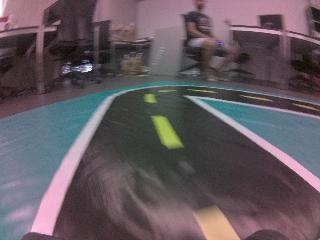
\includegraphics[height=0.50\textwidth]{experiments/11296.jpg}
  \end{minipage}%
  \begin{minipage}{.50\textwidth}
      \centering
      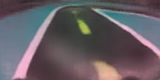
\includegraphics[width=0.60\textwidth]{experiments/11296.png}
  \end{minipage}
  \captionof{figure}{(Left) An image from the real world as seen by the DonkeyCar camera. (Right) The reconstructed image produced by the \textit{real VAE}.}
  \label{fig:realvaeexample}
% \end{figure}
% \begin{figure}
  \begin{minipage}{.50\textwidth}
    \centering
    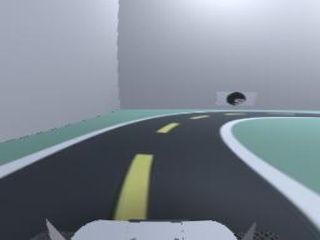
\includegraphics[height=0.50\textwidth]{experiments/1160.jpg}
  \end{minipage}%
  \begin{minipage}{.50\textwidth}
      \centering
      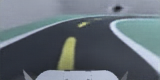
\includegraphics[width=0.60\textwidth]{experiments/1160.png}
  \end{minipage}
  \captionof{figure}{(Left) An image from the simulator as seen by the DonkeyCar camera. (Right) The reconstructed image produced by the \textit{simulated VAE}.}
  \label{fig:simvaeexample}
\end{figure}

\section{RL Algorithm}

\subsection{Reward Function}

Designing a reward function that is effective both in simulation and in the real world is challenging given the fundamental differences between simulated and real world environments. Indeed, in simulation, the environment can provide supervision and useful information such as the position of the car and the speed, that can be used to shape the reward function to guide the training. In our real setup, instead, the DonkeyCar can only leverage information coming from the camera. In particular, we consider the following reward function for both environments:

\begin{equation}
	\label{eq:realreward}
	r_t = 1 + \textit{throttle\_reward} + \left\{\begin{matrix}
		if \textit{done} & \textit{reward\_offtrack} \\ 
		else & 0  
	\end{matrix}\right.
\end{equation}

The first term is a constant bonus for each timestep, that encourages the agent to stay \textit{alive}, i.e. to stay on track in order not to abort the episode prematurely. The second term, i.e. \textit{throttle\_reward} $= (\textit{throttle} - \textit{min\_throttle}) / (\textit{max\_throttle} - \textit{min\_throttle})$, which encourages the agent to go as fast as possible. However, for simplicity and to reduce training time especially in the real world, we keep the throttle constant such that the second component is always zero. Finally, the agent receives a big negative reward (\textit{reward\_offtrack} $= -10$) when it goes offtrack. In simulation, this check is automated and corresponds to a cross-track error (XTE) greater than 3 (i.e., all the car is out of track with all four wheels), while in the real environment the episode is stopped manually when the car goes offtrack. Otherwise, when episode finishes without the car going offtrack (1000 timesteps pass since the beginning of the episode), the agent is not rewarded nor it gets a penalty.

%The reward function designed to work in simulation consists of four parts. The first one is a single point gained by the agent for every step made, intending to improve the length of the path as much as possible. Secondly, a throttle reward term increases the reward by a value proportional to the throttle to encourage the agent to drive as fast as possible. Moreover, a cross-track error penalty is proportional to the distance of the car from the center of the roadway that disincentives the agent as soon as it moves away from the center. Finally, as soon as the agent crashes or exceeds the maximum cross-track error allowed a big penalty is given. Thus, the reward function to be maximized is composed as follows:
%
%\begin{equation}
%  \label{eq:stdreward}
%    r_t = 1 + throttle\_reward + cte\_penalty + \left\{\begin{matrix}
%    if done & crash\_error \\ 
%    else & 0  
%    \end{matrix}\right.
%\end{equation}
%
%In our setup, the throttle is kept constant for the purposes of this thesis.
%The reward function described above is used to test our simulated algorithm and as a starting point, however, we need to adapt it such that it can work also in the real world where the cross-track error is not available. To tackle the issue we simply remove the CTE penalty, even though this will lead to a major problem of shaky motion as described in the next section. The final reward function that has proven to work in both environments and that we will use in the following training procedures is computed as follows:
%
%\begin{equation}
%  \label{eq:realreward}
%    r_t = 1 + throttle\_reward + \left\{\begin{matrix}
%    if done & crash\_error \\ 
%    else & 0  
%    \end{matrix}\right.
%\end{equation}
%
%Since we want real and simulated version of our agent as similar as possible, Equation \ref{eq:realreward} is finally used in both cases.

\subsection{Training the RL Agent in Simulation}

%As a baseline for our RL algorithm, we used the source code provided by \citet{learning-to-drive-in-5-minutes} as a baseline. His algorithm allows the training of many RL algorithms, including the SAC of our interest, of both simulated and real-world agents, however, training on simulation with communication being over the internet is more computationally expensive and more prone to errors. Thus, for the simulation, we refactor the algorithm such that the communication happens locally. Moreover, his algorithm uses an AE which needs to be changed with the more performant VAE chosen above. 

In simulation, we evaluated different \textit{reset strategies} in order to understand how the performance of the RL agent varies. In order to define the different reset strategies we rely on \textit{checkpoints} placed along the track (see Figure~\ref{fig:usitracksim}). In total there are seven checkpoints, distributed in this way: three of them are in the straight road, one checkpoint is in the middle of the first right curve and one at the end; then, there is another in the middle of the left curve and one at the end of the last but one right curve. \matteo{Maybe identify each checkpoint in the figure with a name.}

Based on such checkpoints we define the following reset strategies with various levels of human intervention, considering such strategies applied in the real world:

\begin{itemize}
	\item \textbf{Starting Line}: the agent always starts at the starting line when the episode starts. This is the default reset in the DonkeyCar Gym environment. The starting line is placed in the middle of the straight road sector of the track (see Figure~\ref{fig:usitracksim} and Figure~\ref{fig:usitrack}); 
	\item \textbf{Random}: the agent is placed in a random checkpoint every time an episode starts. The idea behind this strategy is to make the trained agent robust w.r.t. the starting point, since starting always from the same position (i.e., the Starting Line strategy) might lead the agent to repeat one sector of the track more often than the others;
	\item \textbf{Closest Checkpoint}: when the episode finishes the agent is placed to the closest checkpoint w.r.t. its position at the end of the episode;
	\item \textbf{All Checkpoints}: in this strategy we keep track of the latest checkpoint the agent was placed in the previous episode and we restart the next episode by placing the agent in the next checkpoint. Once all checkpoints have been \textit{covered}, we restart from the first.
\end{itemize}

If we had to rank such reset strategies by the manual effort required by the human operator when training the agent in the real world, we would rank Starting Line, Random and All Checkpoints in the top positions, since the operator would need to take the car and place it in a position that is potentially far from the position the car went offtrack. On the other hand, the Closest Checkpoint strategy would be the cheapest since the car would need to be placed closely to where it went offtrack.

For each reset strategy we trained a SAC agent by using the pretrained \textit{simulated VAE} trained earlier for 100\textit{k} timesteps, which corresponds to $\approx$ two hours of training on a MacBook without GPU. During training we track different metrics, i.e., the episode length, the episode reward and the success rate. Regarding the success rate, an episode is considered successful if the agent is able to return to the checkpoint it started from \matteo{check}. Figure~\ref{fig:agentresults} shows the results of the training process for the four agents. Each plot shows the respective metric averaged over 100 episodes. For example, each point in Figure~\ref{fig:agentresults}.a is the episode length averaged over the previous 100 episodes. 

%To train our agents, we need to define what is the best strategy in terms of the starting point. We identified four main options, the first one lets the Donkey start always at the starting line, the second option starts the Donkey from a random checkpoint, the third one at the latest checkpoint reached in the previous episode and finally, the last option makes it start from all checkpoints cyclically. Defining in simulation which is the best strategy can save computational time in real-world training. To identify which one eventually converges more quickly and if it does, 4 different agents were trained, one for each option aforementioned. The quality measures to evaluate the trained agents, illustrated below in Figure \ref{fig:agentresults}, are the \textit{Episode success rate} that shows how many laps have been completed on average during the training, the \textit{Episode Reward mean} and the \textit{Episode Length mean}. All the models have been trained for 100k iterations which correspond to $\approx 2$ hours of training. \textit{ Agent 1} started each lap at a random checkpoint,\textit{ Agent 2} started always at the starting line,\textit{ Agent 3} at the latest checkpoint reached during the last episode, and, finally,\textit{ Agent 4} cyclically uses all the checkpoints.

\matteo{Lines in Figure 5.3 are thin, I would make them thicker. Moreover, the yellow line is not visible; I would use another color.}

\begin{figure}[h]
  \centering
  \begin{subfigure}{.45\linewidth}
      \centering
      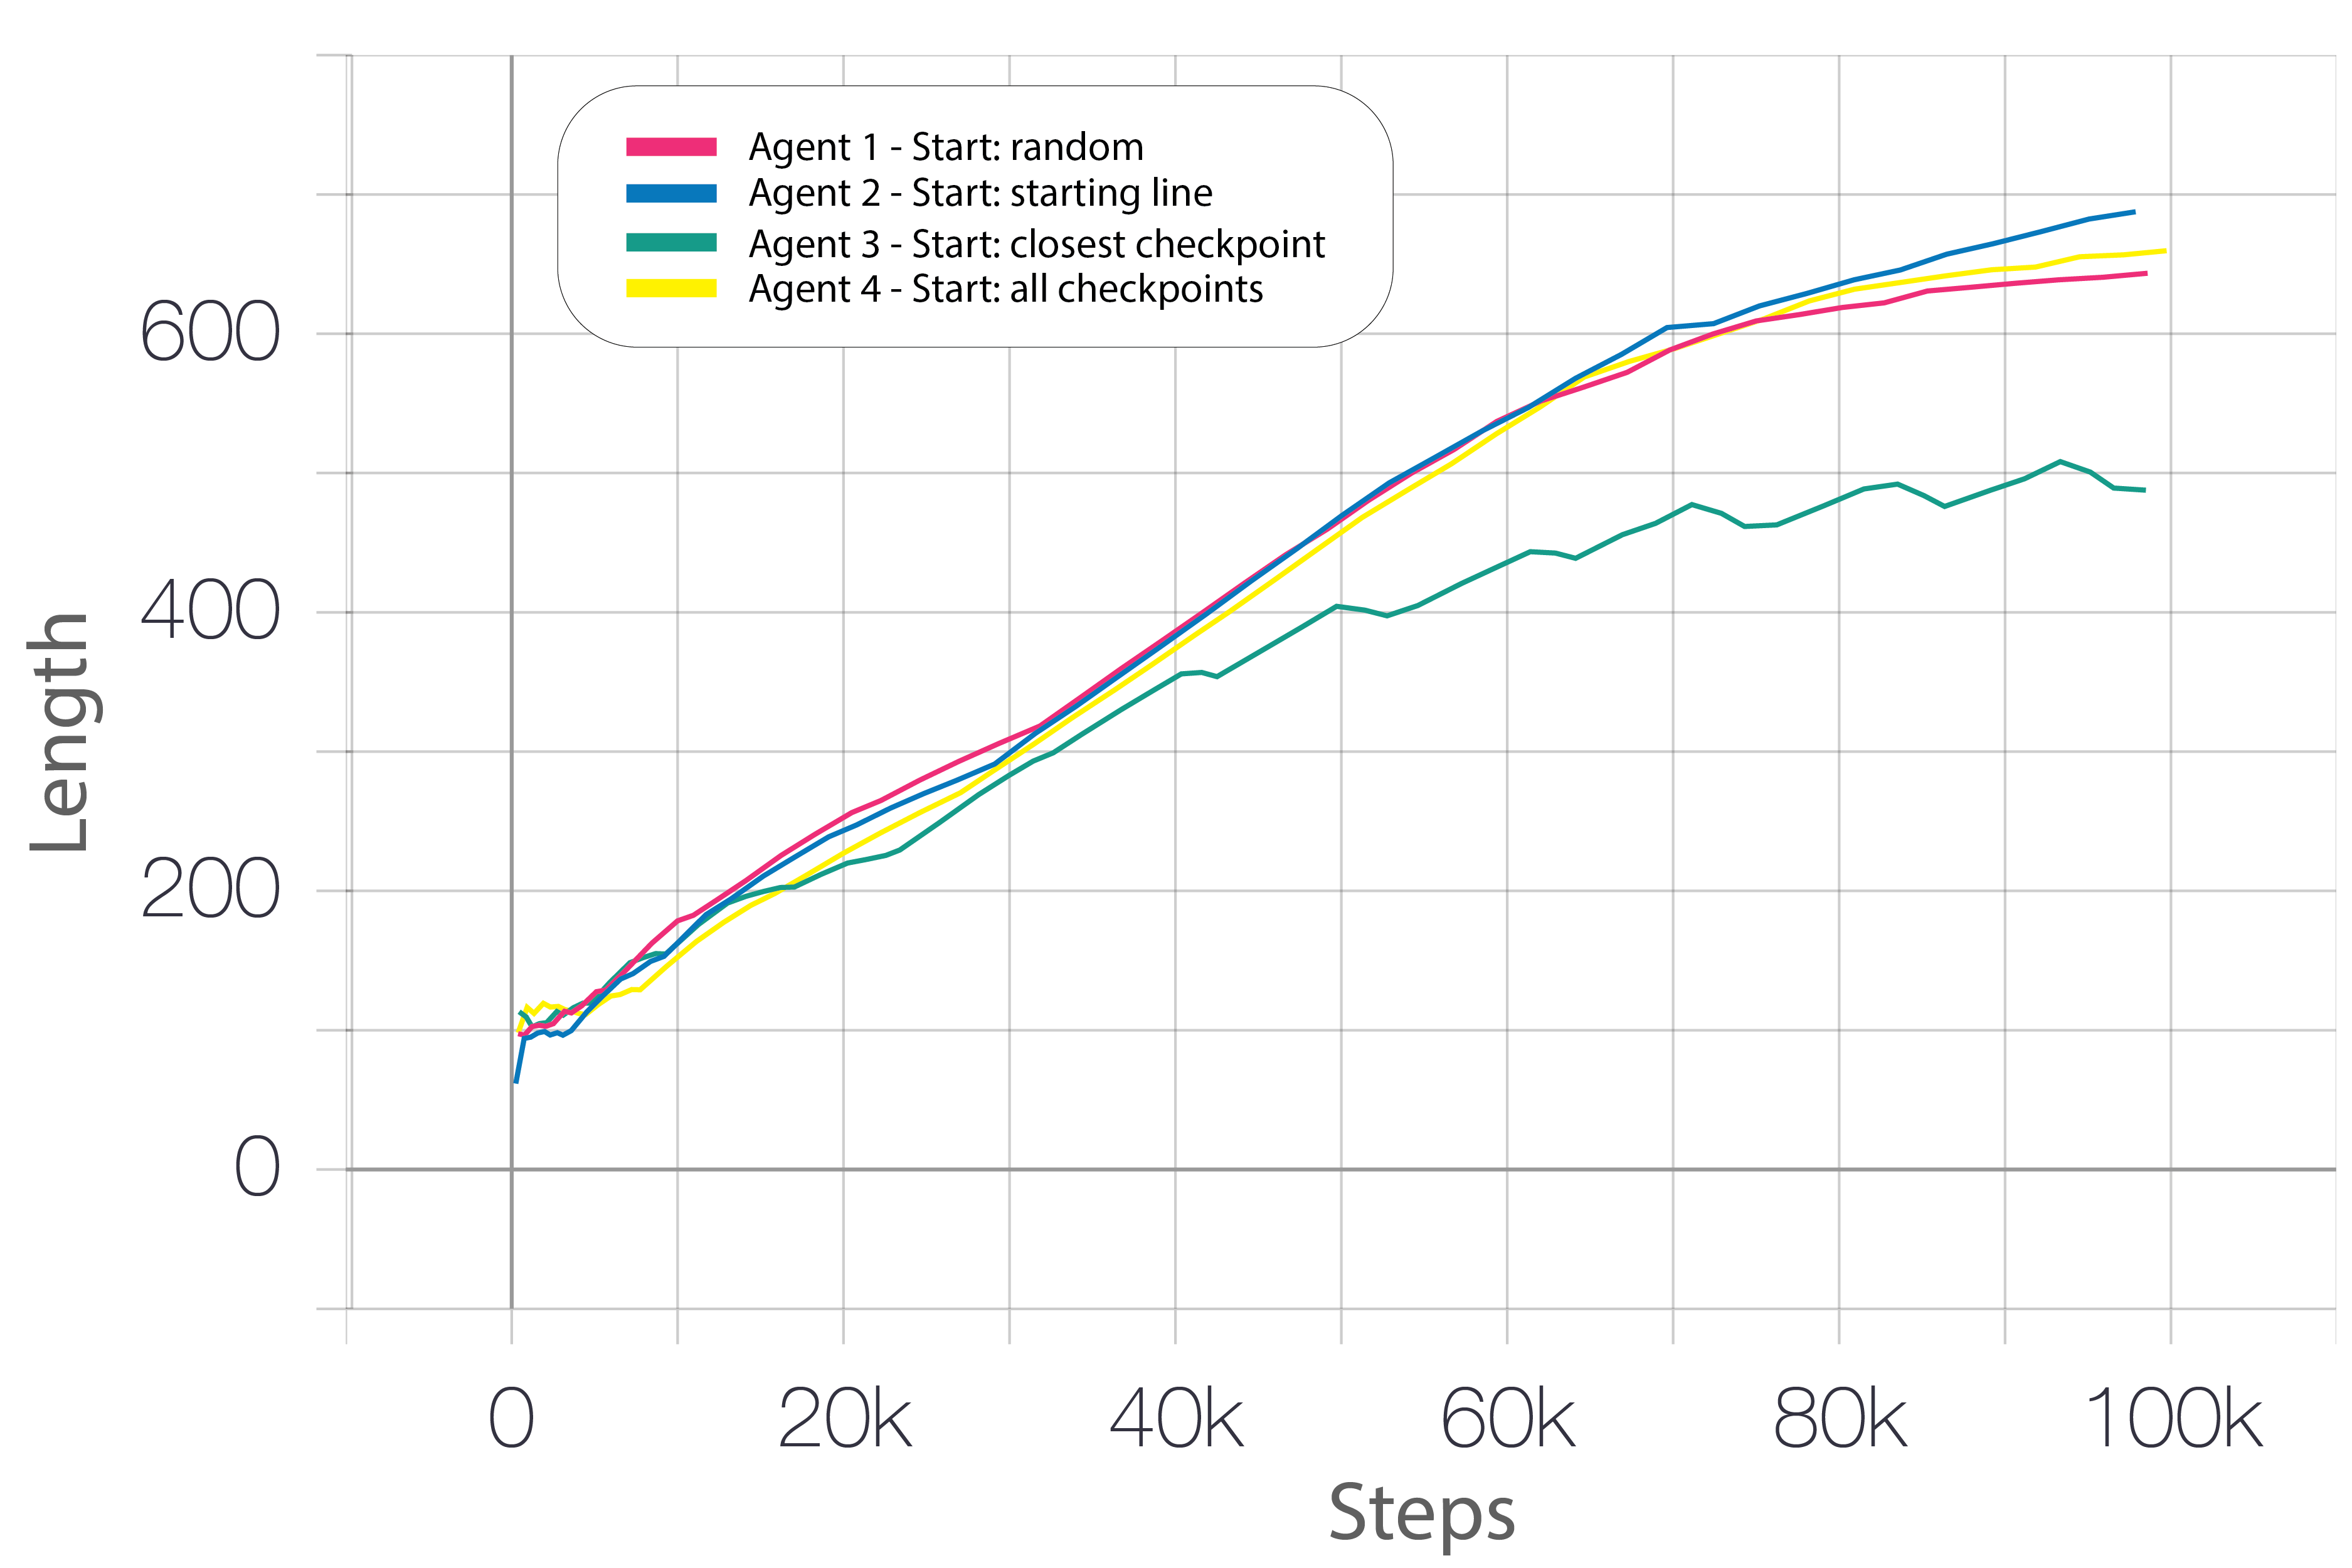
\includegraphics[width=1\textwidth]{experiments/len_mean.png}
      \caption{Mean episode length}\label{fig:len}
  \end{subfigure}%
      \hfill
  \begin{subfigure}{.45\linewidth}
      \centering
      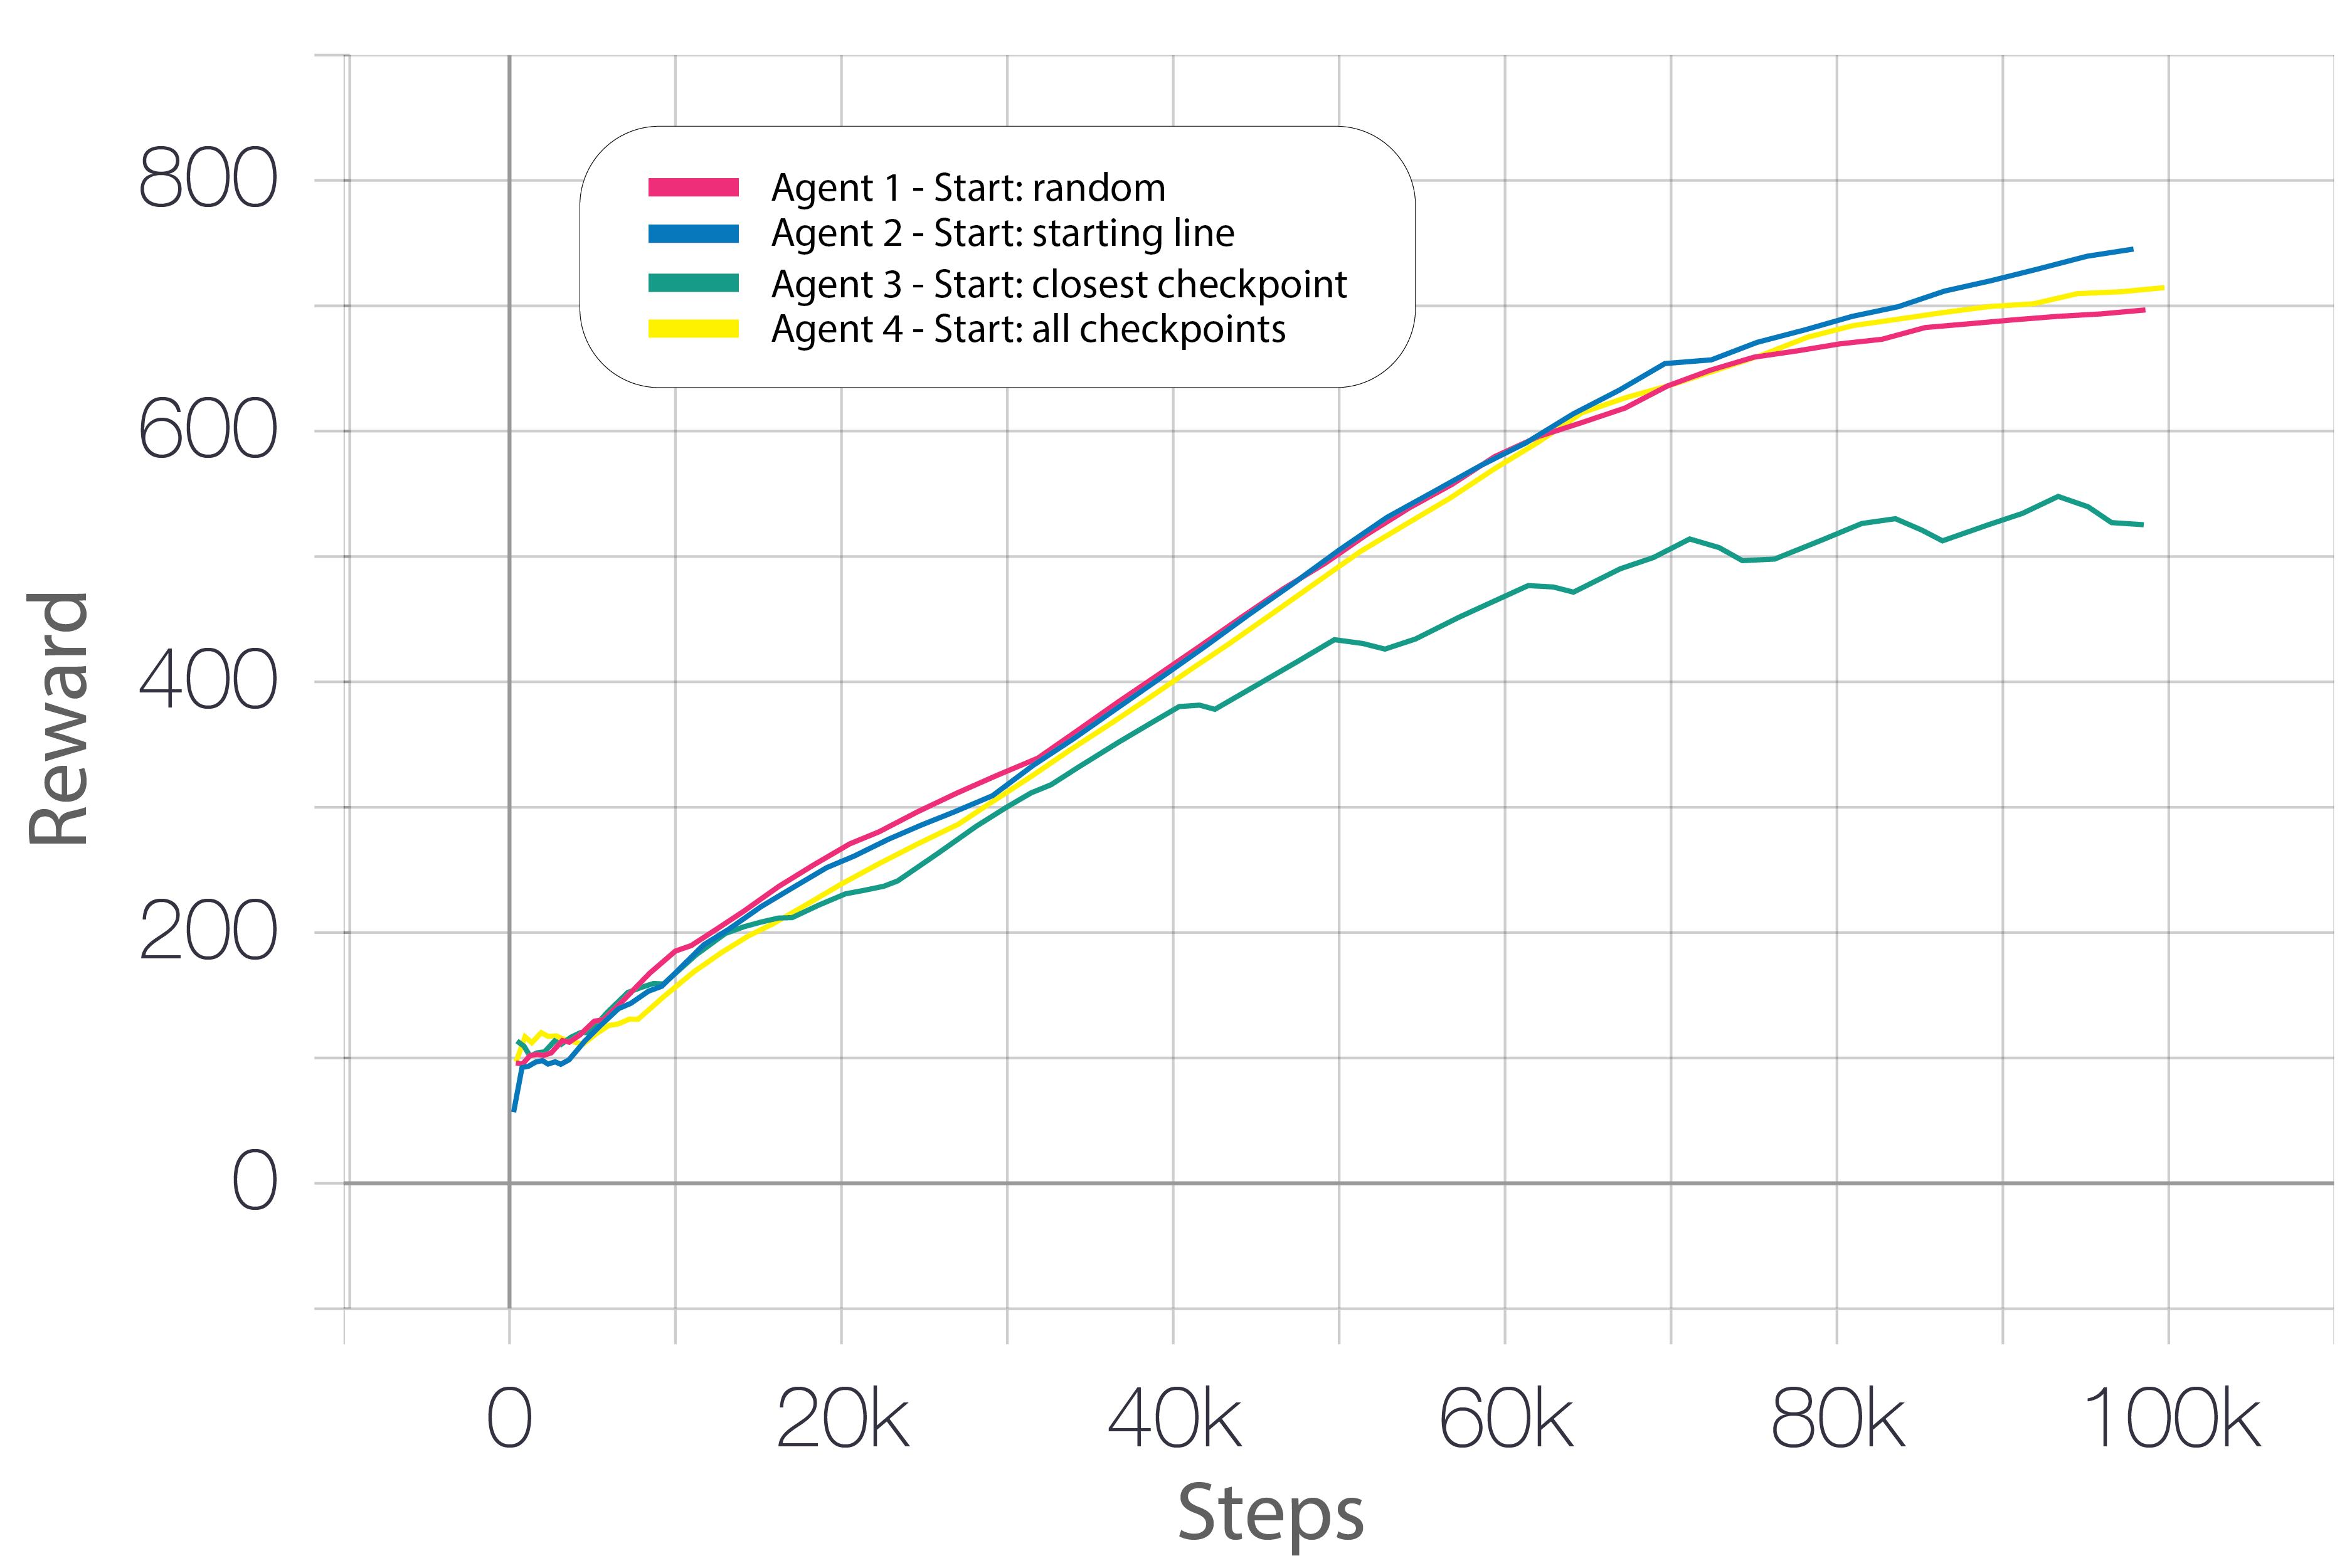
\includegraphics[width=1\textwidth]{experiments/rew_mean.png}
      \caption{Mean episode reward}\label{fig:rew}
  \end{subfigure}
  
  \bigskip
  \begin{subfigure}{.45\linewidth}
    \centering
    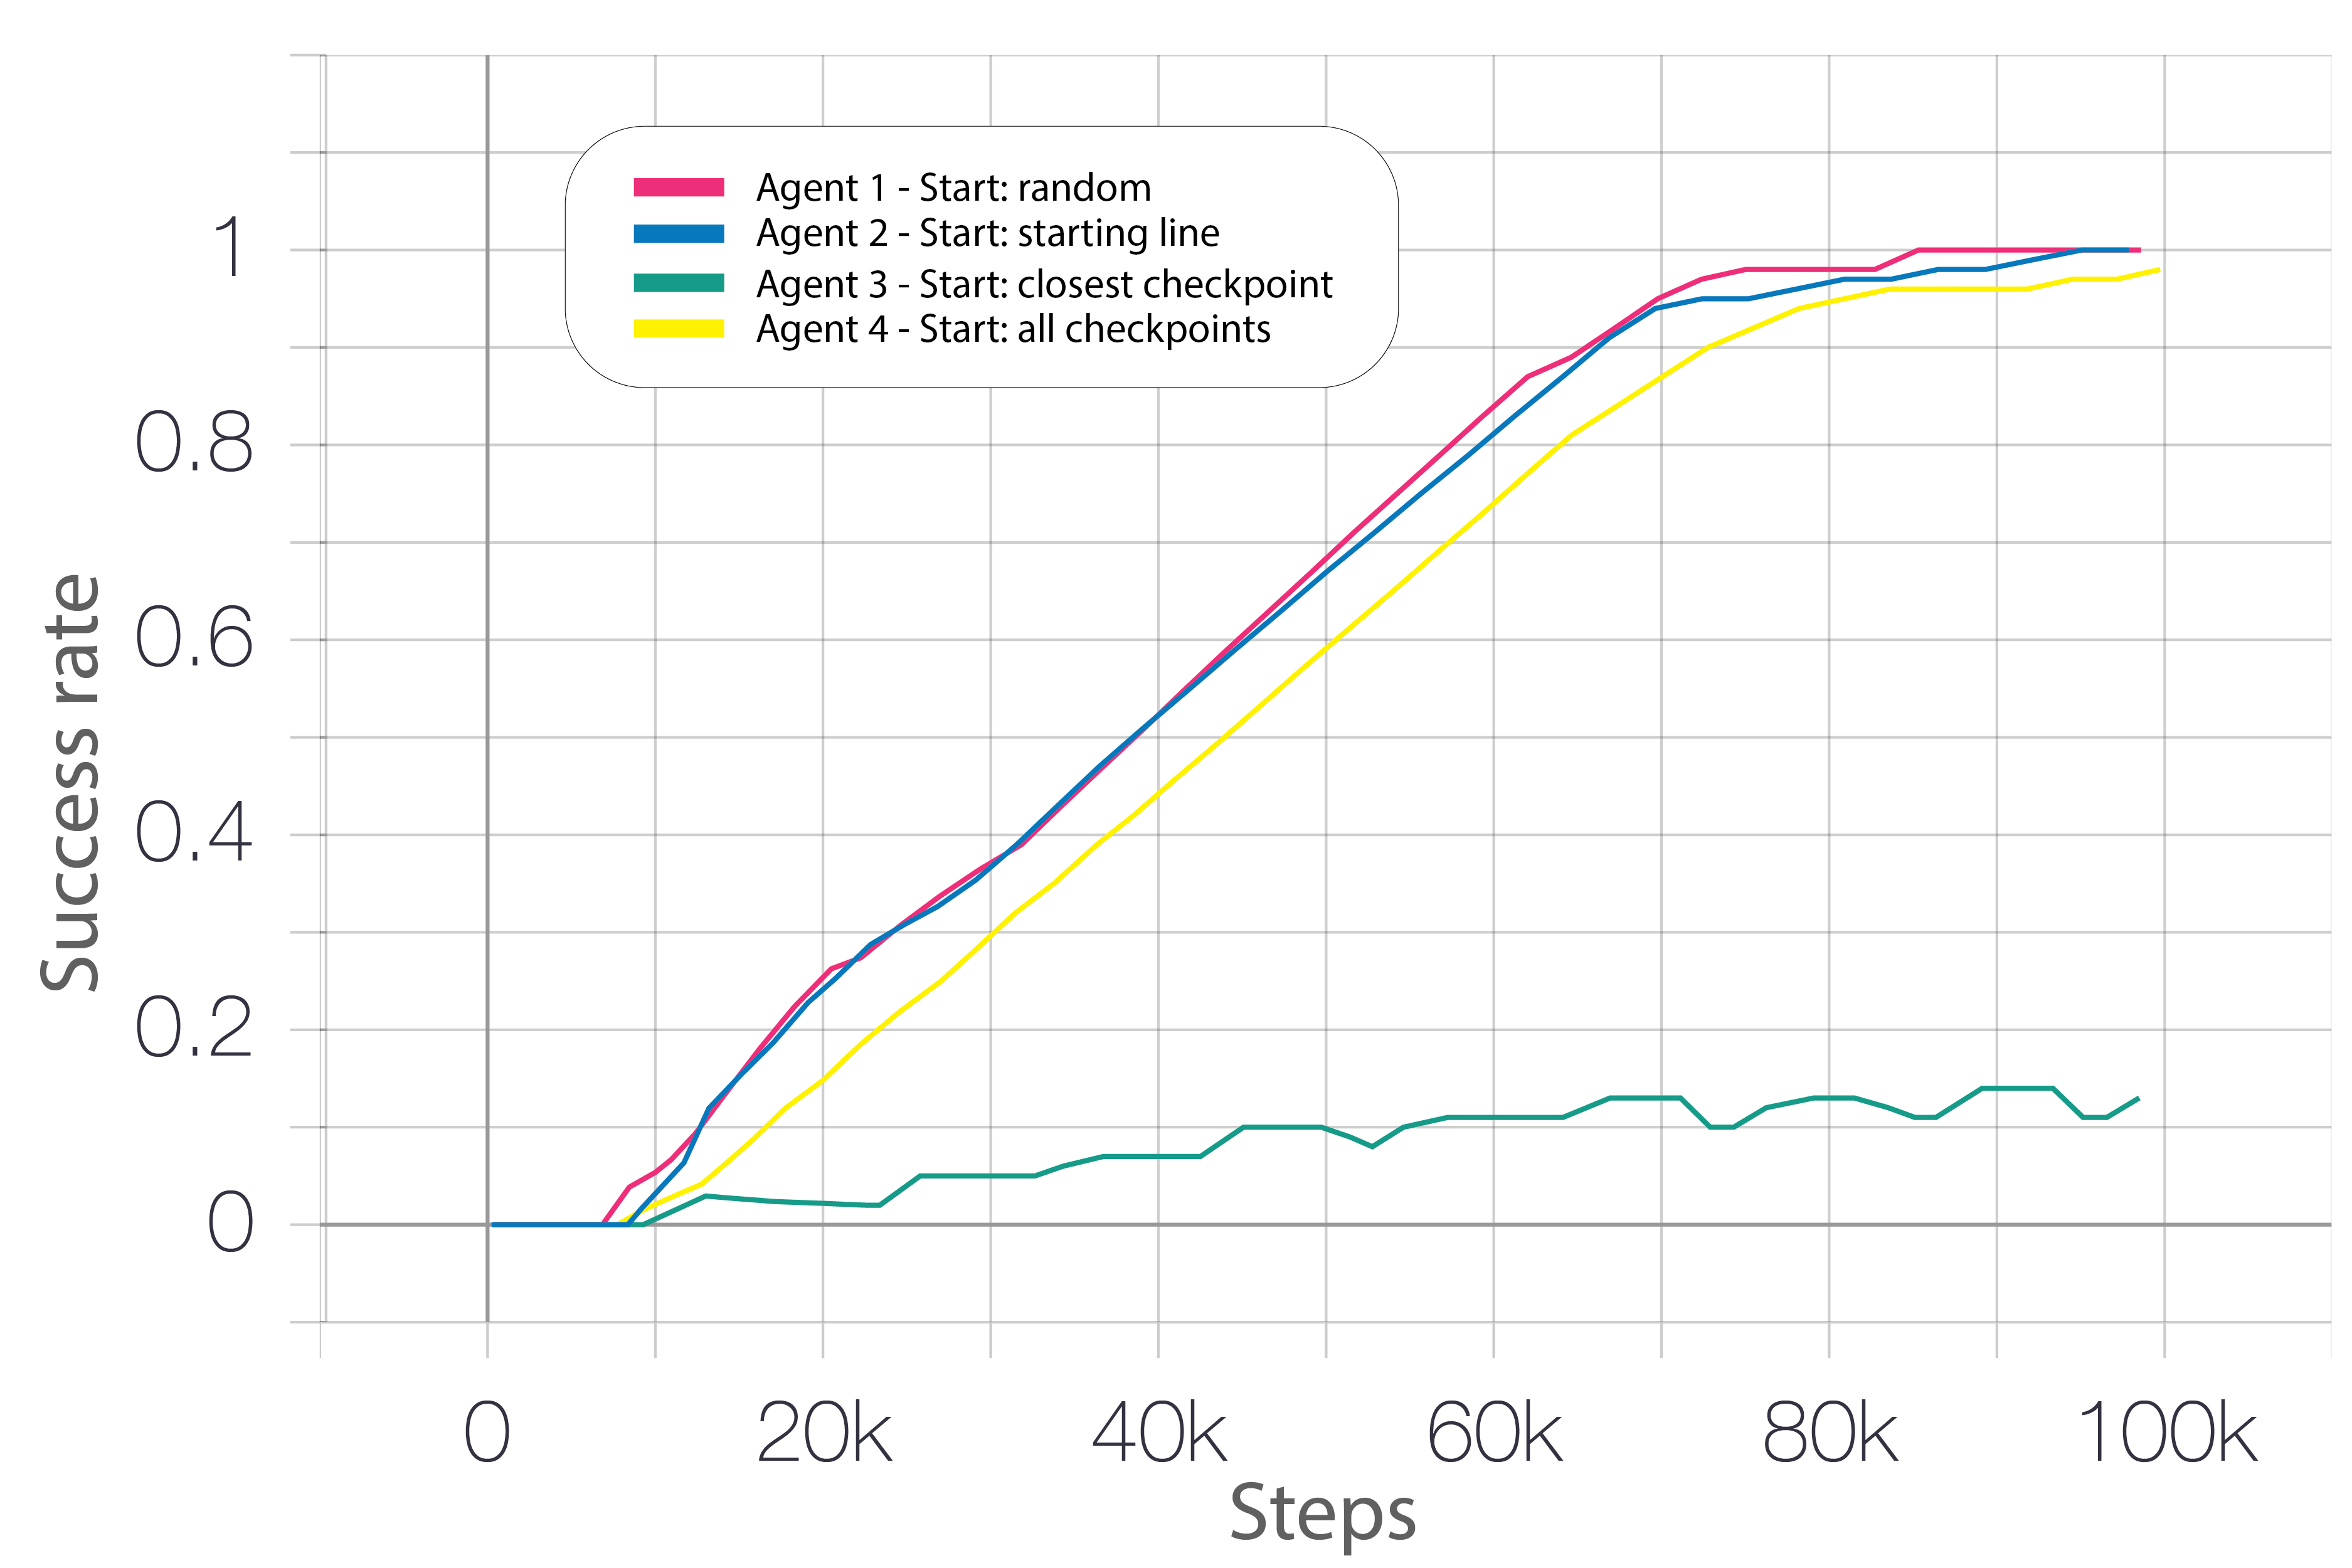
\includegraphics[width=1\textwidth]{experiments/success_mean.png}
    \caption{Mean success rate}\label{fig:succ}
  \end{subfigure} 
  \caption{Agents trained in simulation. Each agent has been trained with a different reset strategy for 100k steps.}
  \label{fig:agentresults}
\end{figure}

%During our experiments, we noted that, in the best case, a lap may take $\approx 350$ iterations to be completed. 

From the figure we can see that, for most strategies, the agent is able to reliably complete the task, except for the Latest Checkpoint strategy. The first two plots show the same trend for all agents; indeed, the reward function is directly linked to the episode length. Interestingly, although for the successful strategies the mean success rate converges at the end of training, which means that the agents are able to consistently finish the lap, the reward, and the episode length, keep increasing. The reason is that the agent is encouraged by the reward function to drive slowly while staying on track. Indeed, one way of slowing down is to learn a zig-zag trajectory, which is the way the agent learns to drive. 

Another interesting result is the one achieved by the Latest Checkpoint strategy. Indeed, following such reset strategy the agent is not able to learn how to drive around the track, achieving a negligible 10\% success rate. However, if we observe both the mean episode length and the mean episode reward plots (i.e. Figure~\ref{fig:agentresults}.a and Figure~\ref{fig:agentresults}.b) we can see that the respective value increases over time. In order to understand this particular behaviour, we took the trained agent and tested it on the same physical track. We observed that the agent found a \textit{blind-spot} where the simulator does not accurately measure the XTE. Figure~\ref{fig:bug} shows the sector in the track where the DonkeyCar goes offtrack (such position is close to the last but one right curve). Essentially, the agent goes offtrack in a position where the XTE is not accurately computed which means that the episode is not terminated and the agent is free of roaming in the scenario, without realizing being offtrack but accumulating reward points nonetheless. This behaviour can be observed only with this reset strategy. The reason is that, when the agent reaches the checkpoint before the last but one curve on the right, it cannot easily overcome the very challenging curve. Instead, it is easier for the agent to turn left in the exact positions where the XTE computation does not signal the end of an episode.

%The agents are all able to successfully learn to drive with a strict maximum CTE (3) except for \textit{Agent 4} which started new laps from the latest checkpoint. Two interesting shreds of evidence come out of those pieces of training. The first one is that even though the success rate mean approaches $100\%$, meaning the agents can consistently finish laps, the reward mean keeps growing. This shows a limitation in the reward function used, in fact, the agent gets a reward for every step and hence it learns to finish the lap following the longest path it has discovered. Moreover, the best way to lengthen the path is a zig-zag trajectory that allows also a doubling of the reward per lap. Secondly, the agent that starts at the latest checkpoint keeps improving the reward up to more than an equivalent completed lap, however, it never finishes a lap as described in Figure \ref{fig:succ}. 
%The reason behind this strange behavior is that the agent found a bug in the simulator used, as shown in Figure \ref{fig:bug}. Essentially, there is a little spot, off track, close to the steepest turn where the CTE is not correctly detected by the simulator, and consequently, the episode is not terminated. The reason why this behavior only happened with this agent lies in the training modality. When the agent reaches that checkpoint, he cannot easily reach the next checkpoint given the toughness of the turn, instead, it finds it easier to explore the bugged spot which is almost right in front of it when it approaches the turn.

\begin{figure}[h]
  \begin{center}
    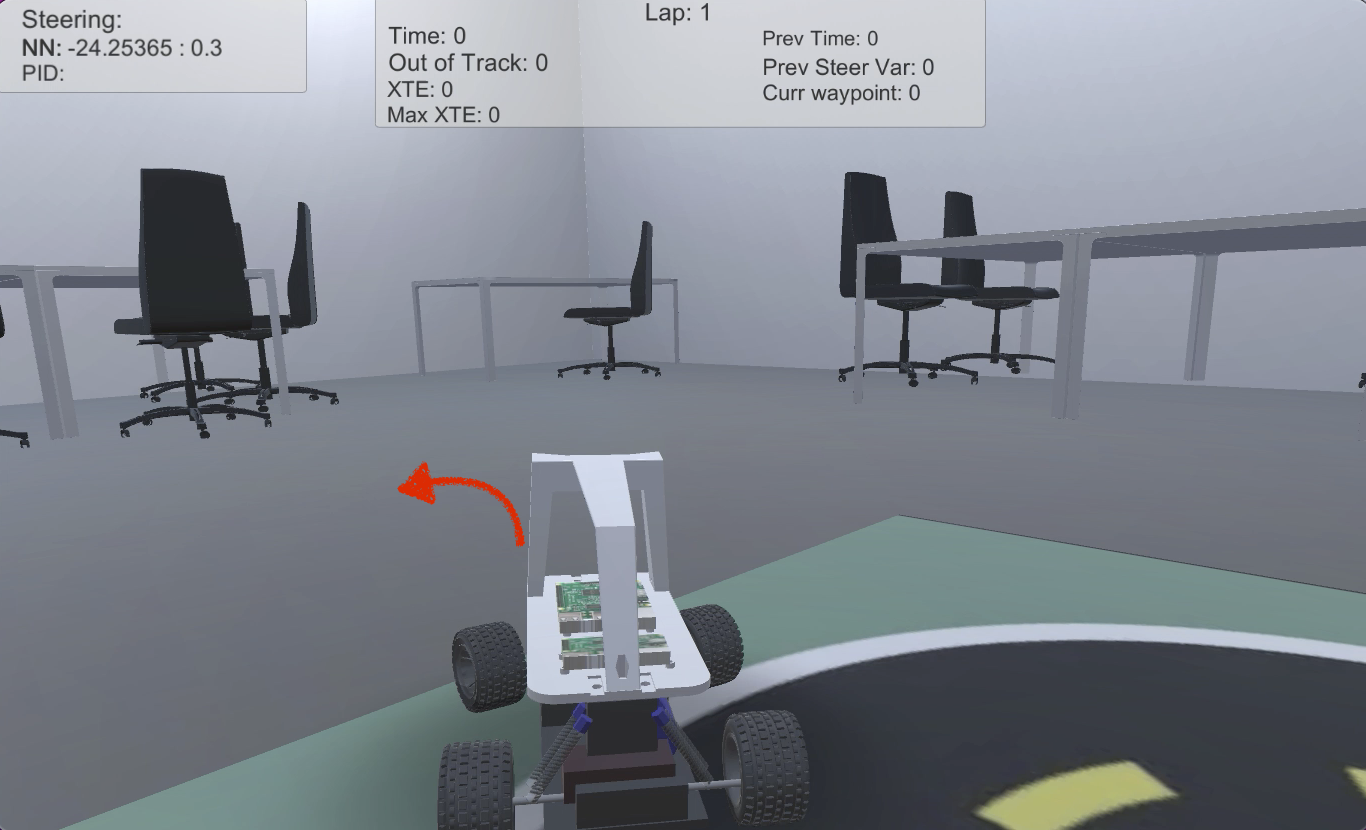
\includegraphics[width=0.50\textwidth]{experiments/bug.png}
  \end{center}
  \caption{Blind-spot in the simulator being exploited by the agent}
  \label{fig:bug}
\end{figure}

After training, we took the final agents for each reset strategy and tested them on the same track. In particular we executed each agent 10 times and enabled deterministic actions for the SAC algorithm, which means that, given an observation, the trained stochastic policy selects the action with the highest probability. Indeed, we executed each agent multiple times to account for the randomness of the simulator. A lap is successful when the car is able to return to the starting checkpoint according to the reset strategy \matteo{check}. The results of such experiments are shown in Table~\ref{tab:simagent}.

%To further test the trained agents, for 10 laps it is measured how many times a lap has been completed by each agent, how many times the agents crash, and finally how many times they exceed the roadway but can recover and finish the lap without crashing. The result are presented in Table \ref{tab:simagent}.

\begin{table}
  \centering
  \begin{tabular}{|c|c|c|c|c|c|}
  \hline
  AGENT & \# OOT & \# OBE & SUCCESS RATE & MEAN EP. LENGTH & MEAN EP. REWARD \\ \hline
  1 (R) & 0 & 0 & 1 & 595 & 644 \\
  2 (SL) & 0 & 4 & 1 & 599 & 647  \\ \hline
  3 (AC) & 0 & 0 & 1 & 624 & 676 \\
  4 (CC) & 10 & 29 & 0 & 460 & 495  \\ \hline
  \end{tabular}
  \caption{Agents results averaged over 10 runs. \matteo{In the plots Agent 4 is the one trained with AC while here it is the one trained with CC.}}
  \label{tab:simagent}
\end{table}

During testing we measure the average Out of Track (OOT) events (second column), i.e., the number of times the agent goes offtrack, the average Out of Bound (OOB) events (third column), i.e., the number of times the measured XTE is greater than 2, the average success rate (fourth column) and the average episode length and episode reward (respectively fifth and sixth columns). An OBE event means that the agent momentarily exists from the roadway but it is able to recover. From the results we can see that all agents, except the agent trained with the Closest Checkpoint strategy, are able to successfully complete the ten laps. Since the average reward is comparable across the successful strategy, no clear winner reset strategy to be used in the real world training emerges.

%From the results is evident, excluding \textit{Agent 4} because of the simulator's bug, that three agents learned to successfully drive and in most cases, they always stay entirely on track without the need for any additional sensor and with the only problem of the shaky driving which is still acceptable for the purposes of this thesis, in most cases, they never get out of the track, and if they do they can recover consistently.

\subsection{Training the RL Agent in The Real World}

Since no clear winner among the reset strategies emerged from the experiments in simulation, all the reset strategies, including the Closest Checkpoint one, are viable to be tested in the real world. However, we only experimented with the default reset strategy, i.e. the Starting Line strategy, and the most convenient strategy in terms of supervision effort, i.e. the Closest Checkpoint strategy. Indeed, we trained two agents, i.e., one for each strategy, with the SAC algorithm and by using the pretrained \textit{real VAE}. Each agent was trained for $\approx$ 30 minutes.

\begin{figure}[h]
	\centering
	\begin{subfigure}{.5\linewidth}
		\centering
		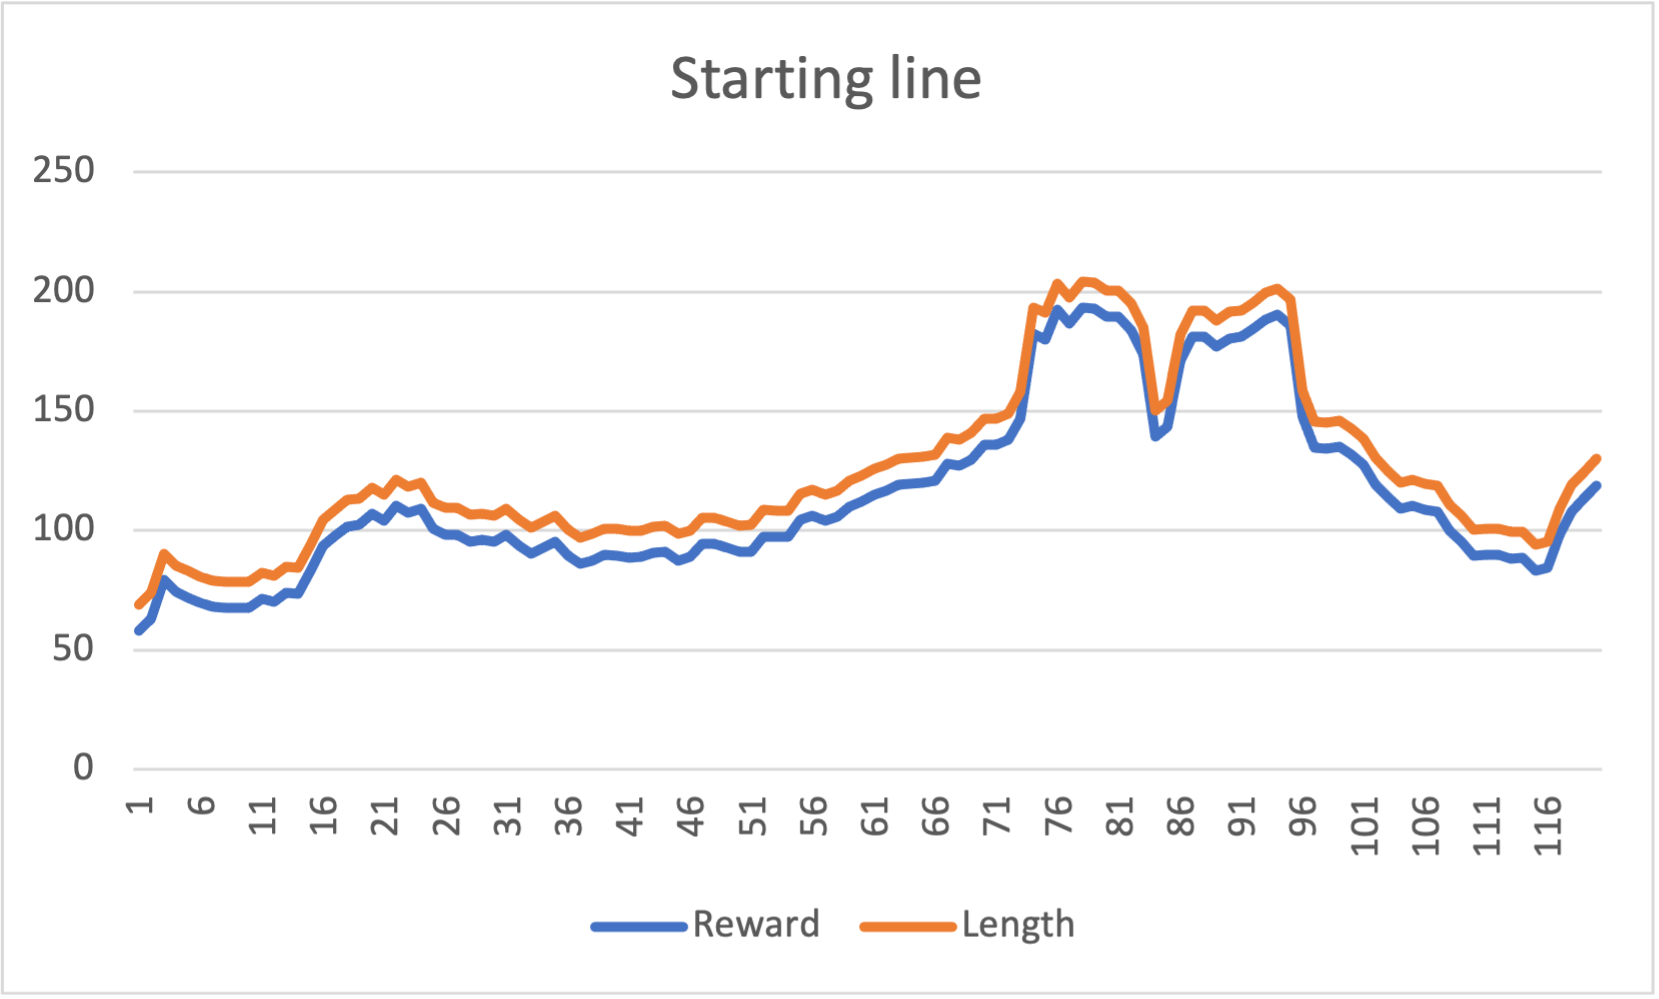
\includegraphics[width=1\textwidth]{experiments/badrealagentstart.png}
		\caption{Mean episode length and reward: Starting Line strategy}\label{fig:rlen}
	\end{subfigure}%
	\hfill
	\begin{subfigure}{.5\linewidth}
		\centering
		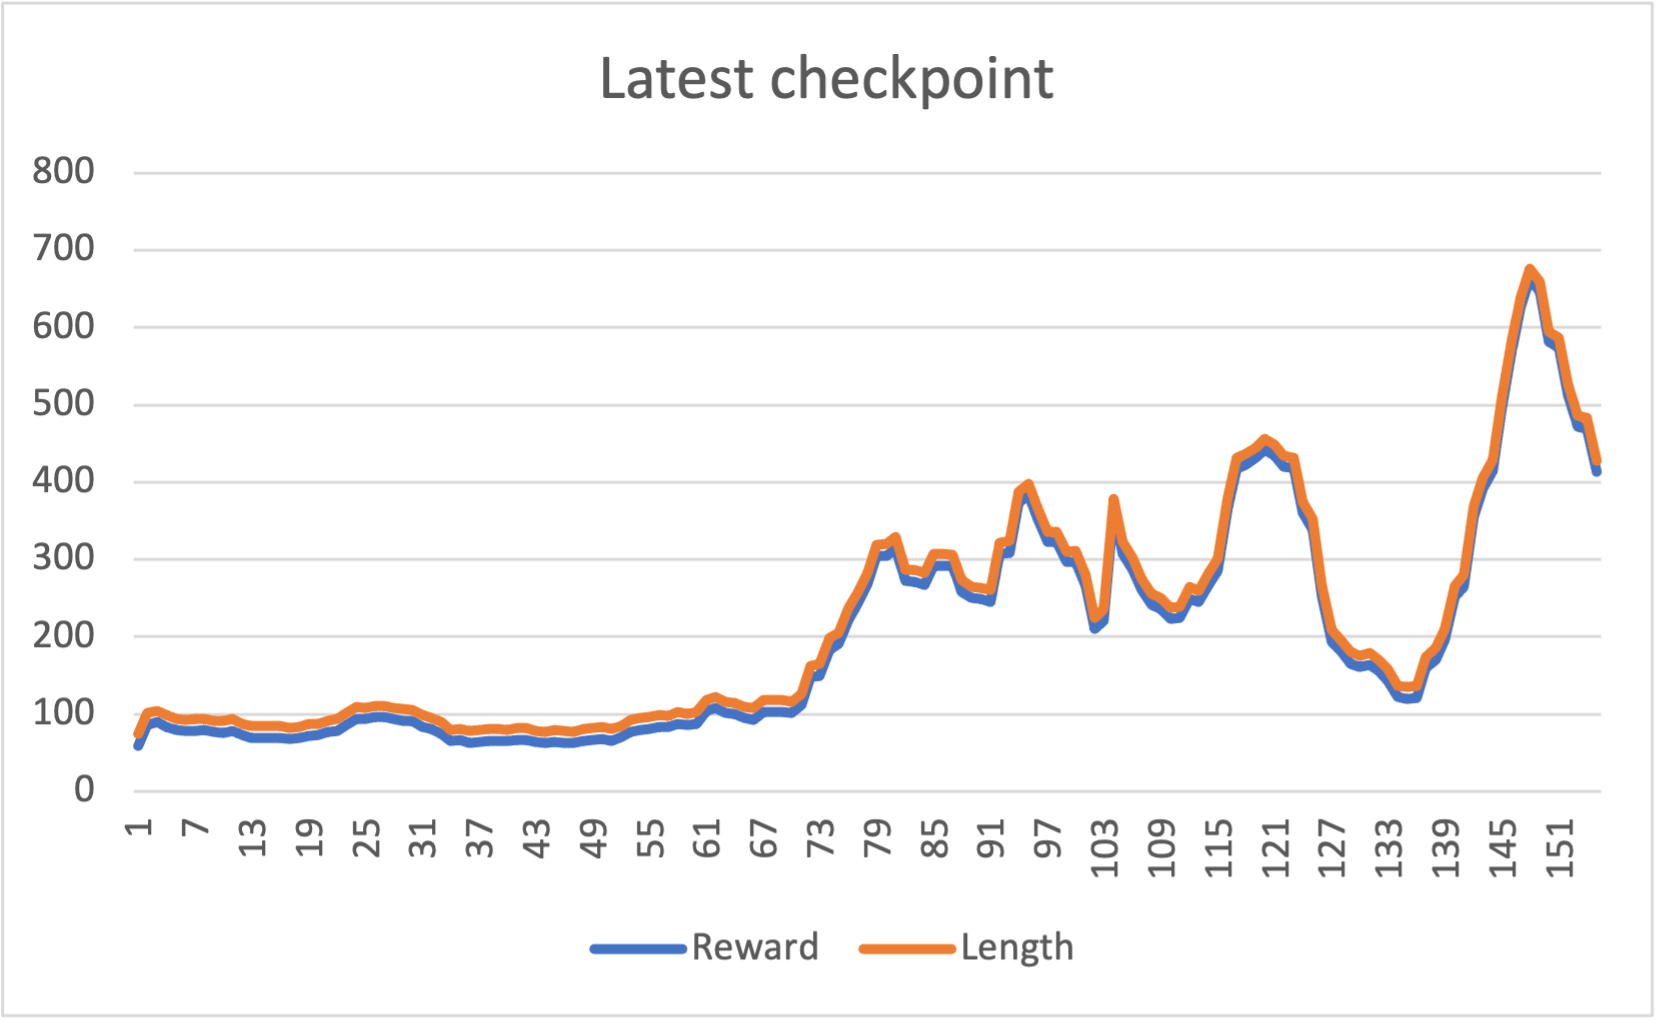
\includegraphics[width=1\textwidth]{experiments/badrealagentlatest.png}
		\caption{Mean episode length and reward: Closest Checkpoint strategy}\label{fig:rrew}
	\end{subfigure}
	\caption{Agents trained in real world with the Starting Line strategy (left) and Closest Checkpoint strategy (right). \matteo{Plots are not in scale ($y$-axis different), difficult to compare the results.}}
	\label{fig:realresult}
\end{figure}

Figure~\ref{fig:rlen} shows the training curves for the two agents. The two lines (i.e., $y$-axis) for each plot show the mean reward and the mean episode length across the previous 100 episodes \matteo{check}, while the $x$-axis shows the number of episodes, i.e., the training time.

From the plots we can see that the agent that learns with the Starting Line strategy did not manage to achieve a good reward given a budget of $\approx$ 100 episodes. On the other hand the other agent with the Closest Checkpoint strategy was able to achieve 100\% more reward with the same budget (i.e., 400 average reward vs 200 average reward). Therefore, after 100 episodes we decided to stop the training of the first agent, in order to save time. Instead, we carried out the training of the most promising agent, in order to observe further improvement. In total, such agent was trained for 45 minutes, taking approximately 30 minutes to complete a lap and by the end it was able to complete two laps (notice that in the real world an episode terminate successfully when 1000 timesteps pass, which correspond to $\approx$ 2.5 laps).

Interestingly, in the right plot of Figure~\ref{fig:rlen} both the average reward and the episode length show an oscillating behaviour starting at episode 73. Such behaviour can be explained by the different levels of difficulty of the track and by the reset strategy. Indeed, when the agent is placed at the starting line it is able to drive well since the initial part of the track is relatively easy to drive, with a straight line and a smooth right curve. Then, when the agent arrives in the challenging sectors of the track \matteo{which one?}, the agent goes offtrack and restarts in the closest checkpoint. Then, it takes the agent some time to learn how to drive in the challenging part and, as a consequence, the average reward decreases. The reward keeps decreasing until the challenging part is overcome and the it starts increasing again. This oscillating behaviour repeats multiple times during training until the agent is able to drive the challenging part at full speed.

Regarding the difference w.r.t. the Starting Line strategy we suspect that the advantage of the Closest Checkpoint strategy is that, in the latter, the agent is given the chance to learn the challenging part of the track at a low speed, since the agent starts close to it. On the other hand, if the agent always starts at the Starting Line, it is forced to learn the challenging part at full speed, which requires more training time.

To summarize, we were able to train a RL agent in the real world in a reasonable amount of time, i.e. $\approx$ 30 to 45 minutes, by decoupling state learning, which we addressed with a VAE, from policy learning which we tackled with the SAC algorithm. Moreover, we used a custom reset strategy that enabled training of an effective policy.

%To train the real-world agent, instead, the source code provided by \citet{learning-to-drive-in-5-minutes} is kept untouched beside the encoder, with the main goal being to replicate their results but with a more performing VAE as resulted in our tests. Given that in the real world the simulator's supervision is not available, all the strategies tested in the previous section are good candidates to be used, also \textit{Agent 4} strategy that cannot explore anymore the simulator's bug. In fact, in the real world, we only have human supervision that is about stopping the episode as soon as the car exceeds the track boundaries with all 4 wheels, while the server automatically stops the car when it reaches 1000 steps ($\approx 2.5$ laps). From the tests resulted that all the agents, trained with the aforementioned strategies, struggle to learn to drive an entire lap, at least in a reasonable time, except\textit{ Agent 4 }that start his laps at the latest checkpoint reached in the last episode. For the sake of brevity, since they are all equivalent among the failing agents, only the results of the agent that starts always at starting line and fails in learning, as shown in Figure \ref{fig:rlen}.
%
%In figure \ref{fig:rrew}, instead, are shown the performances in the training of the agent starting at the latest checkpoint (equivalent strategy of previous \textit{Agent 4}), which can be considered successful and comparable to simulated agents since it did learn to complete a lap in about 30 minutes and two laps in about 45 minutes. In five to twenty episodes, the first two turns were learned decently and most of the time was spent on the steepest turn. As shown in Figure \ref{fig:rlen}, the graph is characterized by ups and downs, as soon as the car started at the starting line, it learned quickly, then, when the steepest curve was reached it struggled to overcome it and when it eventually did, the length started to increase again. The process was repeated until it was almost consistently able to finish a lap. Furthermore, as soon as the agent learned the steepest turn, it did generalize well on the following turns and little time was spent on them.
%
%Notice that the laying of the car at the latest checkpoint has been intentionally approximate on the area close to the checkpoints. This brought a main advantage, the agent learned quicker since it was able to see the area in front of it from many points of view and this, resulted useful when the car started to cross many checkpoints per episode since the direction from which the car arrived to a checkpoint could vary a lot, it had been trained to drive on many possible trajectories and was able to join the various sections well. Unfortunately, in the real world, more metrics to measure the quality of the driving and to make comparisons with the simulated agents are not available. 

\section{Sim to Real and Real to Sim}

In this section we present an unsuccessful attempt at transferring the agent trained in the real world in simulation (real2sim, or r2s for short). This transfer would be useful in order to better evaluate the real world agent, given the constraints of the physical world. Indeed, in simulation it is possible to generate tracks with any shape and length to test the capabilities of the given agent. Likewise, transferring an agent trained in simulation into the real world (sim2real or s2r for short), would be useful to automate the training process, especially in the reset, and avoid unsafe behaviour of the agent.

%Could not work also because we are only bridging the visual gap, while the physical gap is not addressed (see robot paper cited in testing-rl).

%In this section we present an unsuccessful attempt in driving our simulated DonkeyCar with the real agent trained above. SimToReal (S2R) and vice-versa aims in deploying model trained in one environment to the other. In our case, since the real world environment, in our setup, does not provide enough metrics to benchmark our real world agent, we aim to make it works also in simulation. For example, in order to test the generalization of the real agent would be much easier in simulation where multiple tracks or obstacles can be implemented at a low cost. Another advantage brought by this approach is that an agent trained in simulation, can be moved into the real world and this would result in less expensive training procedures and eventually more robust agents. 

We follow previous work~\cite{stocco-mind} that attempts to bridge the visual gap between simulation and real using image-to-image translation techniques. In particular, we train a CycleGAN~\cite{CycleGAN2017} to translate the images in one domain (real) into the other (simulated) and viceversa. In particular, we used the same hyperparameters of the original paper and trained the CycleGAN architecture for XX epochs \matteo{check}. During training we saved different checkpoints, we visually assessed the quality of the translations for some of them and picked the one with the best-looking translations. Figure~\ref{fig:cycleganexample} shows an example of translations generated by the CycleGAN generators (respectively, s2r generator in Figure~\ref{fig:cycleganexample}.a and r2s generator in Figure~\ref{fig:cycleganexample}.b). The images generated by the CycleGAN generator are called \textit{pseudo}-real or \textit{pseudo}-simulated, since they are translations from one domain into the other.

%The idea is to pre-train a CycleGan \citep{CycleGAN2017} for image transfiguration. In fact, the CycleGan is able to move an image into another domain keeping the original structure unaltered, but applying the style of the other domain as shown in Figure \ref{fig:cycleganexample}. Thus we leverage this property to transform images seen by the simulated camera of the DonkeyCar into what it would see in real world and vice-versa. Then, a real agent will eventually be able to drive on the simulator since it does see pseudo-real images. On the other hand, in order to drive a real car with a simulated agent, our DonkeyCar has not enough computational power, hence it could not run in time a CycleGan, that has millions of parameters, to make the real car see pseudo-simulated images and drive with the simulated agent. However, the problem can be circumvented by training an agent entirely on simulation but with pseudo-real images. After training CycleGAN with our datasets, it is able to transfigure image with high fidelity as shown in Figure \ref{fig:cycleganexample}. In fact, in human eyes they are barely distinguishable. However, even if the result looks good it could not be the case for the AutoEncoder that needs to place similar real and pseudo real images close into the latent space and similarly for similar simulated and pseudo simulated images.

\begin{figure}[h]
  \centering
  \begin{subfigure}{.6\linewidth}
      \centering
      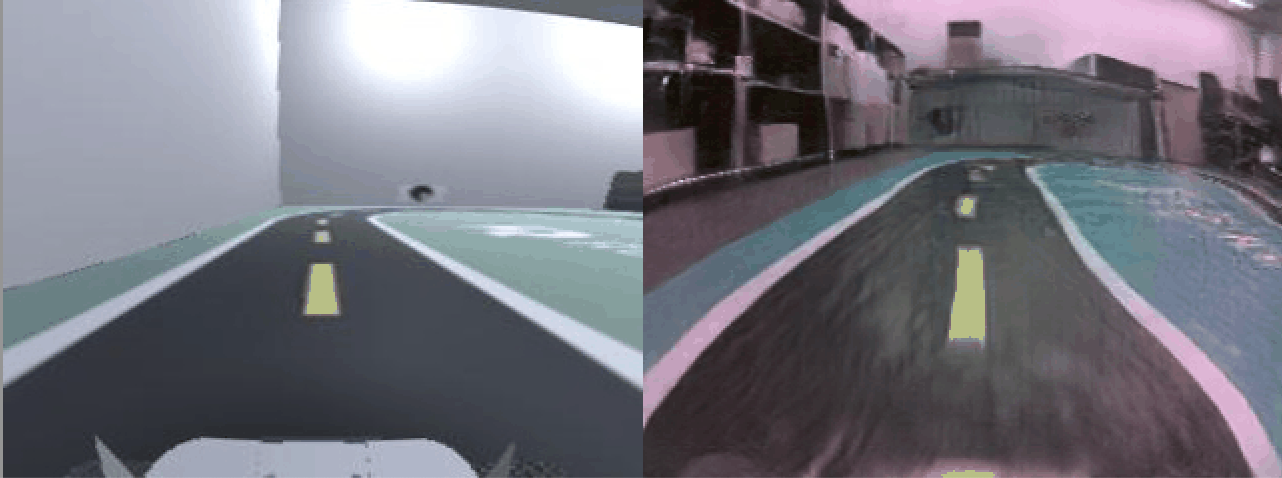
\includegraphics[width=1\textwidth]{experiments/s2r.png}
      \caption{From simulated images to pseudo-real.}\label{fig:s2r}
  \end{subfigure}
      \hfill
  \begin{subfigure}{.6\linewidth}
      \centering
      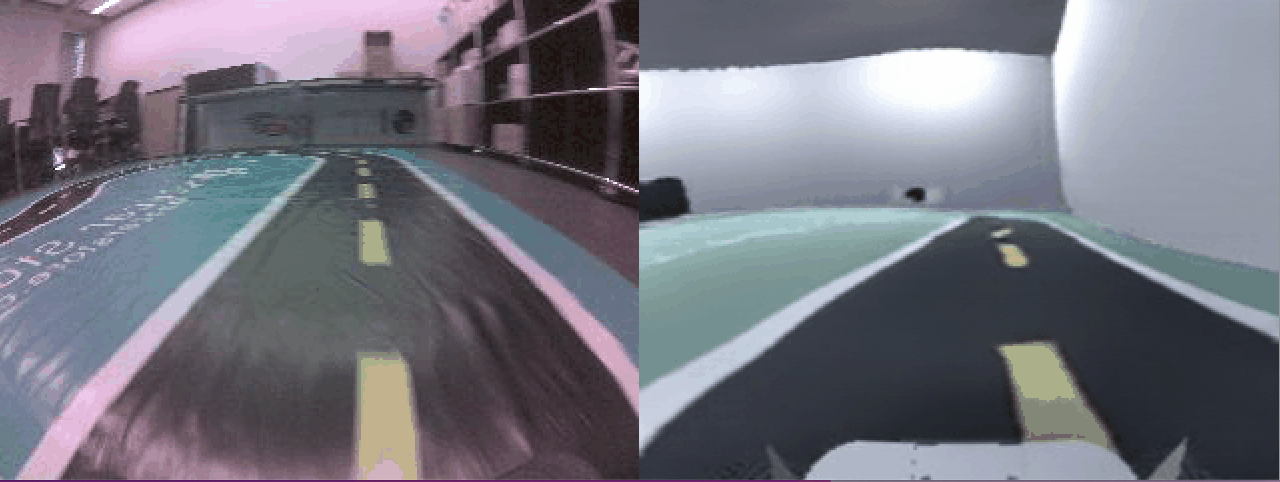
\includegraphics[width=1\textwidth]{experiments/r2s.png}
      \caption{From real images to pseudo-simulated.}\label{fig:r2s}
  \end{subfigure}
  \caption{Translations generated by the trained CycleGAN.}
  \label{fig:cycleganexample}
\end{figure}

Once the CycleGAN architecture was trained, we used it to translate the two test sets of images we collected to evaluate the \textit{simulated VAE} and the \textit{real VAE}. The objective of this preliminary analysis is to understand how the \textit{pseudo} images generated by the CycleGAN are mapped by the chosen VAEs in the two domains w.r.t. the \textit{authentic} (i.e., real and simulated images captured by the camera of the car) images. Indeed, if we want to use the CycleGAN to transfer the trained agent from one domain into the other, we have to translate each image coming from the camera into a pseudo image of the other domain, which is mapped by the VAE into the latent space; only then, the corresponding latent space is processed by the trained policy.

After translating the two test sets we computed the latent space for each image using the two VAEs and then applied the t-SNE dimensionality reduction technique~\cite{tsne} to visualize how the translations are mapped by the encoders w.r.t. the authentic images. The visualization is shown in Figure~\ref{fig:latentpseudo}.

\begin{figure}[h]
  \centering
  \begin{subfigure}{.5\linewidth}
	      \centering
	      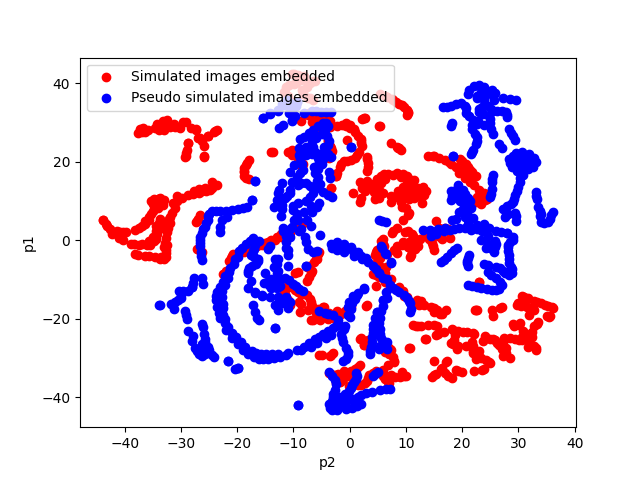
\includegraphics[width=1\textwidth]{experiments/latentr2s.png}
	      \caption{Simulated (authentic) and pseudo-simulated images}\label{fig:latentr2s}
	  \end{subfigure}%
      \hfill
  \begin{subfigure}{.5\linewidth}
	      \centering
	      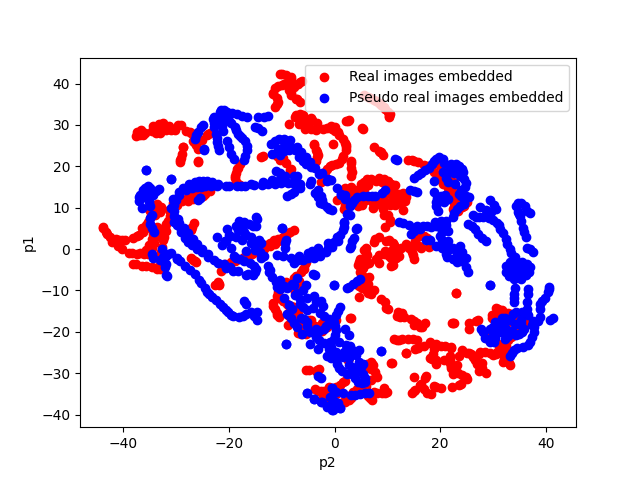
\includegraphics[width=1\textwidth]{experiments/latents2r.png}
	      \caption{Real (authentic) and pseudo-real images}\label{fig:latents2r}
	  \end{subfigure}
  \caption{Latent space visualization: authentic vs pseudo (i.e., translated) images. (Left) simulated VAE, (right) real VAE.}
  \label{fig:latentpseudo}
\end{figure}

Notice that the two test sets are not \textit{paired}. Indeed, both represent images of a lap taken by driving manually along the track in simulation and in the real world. However, despite the images should represent similar situations during driving, we can see that the embeddings do not consistently overlap, both in the r2s case (Figure~\ref{fig:latentpseudo}.a) and in the s2r case (Figure~\ref{fig:latentpseudo}.b). There are some regions, more prevalent in the s2r case, in which the embeddings produced by the VAE overlap for the pseudo and the authentic images, but there are others that are mapped in different regions. This could lead to the trained agent not to act consistently when presented with authentic and pseudo image, since the latent space that will be produced by the VAE will be necessarily different.

In order to understand whether the non-overlap is due to the unpaired dataset, we decided to repeat the previous analysis by creating a paired dataset using the CycleGAN. Indeed, we can use the two generators of the CycleGAN to translate an image from one domain into the other (first step) and then back into the original domain (second step). An example of such \textit{double} translation for both domains is shown in Figure~\ref{fig:examplealigned}.

\begin{figure}[h]
  \centering
  \begin{subfigure}{.33\linewidth}
	      \centering
	      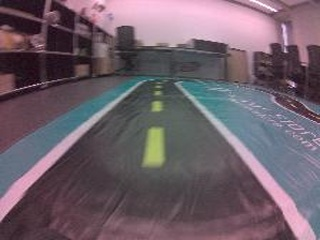
\includegraphics[width=1\textwidth]{experiments/0_.jpg}
	      \caption{Real image}\label{fig:real}
	  \end{subfigure}%
      \hfill
  \begin{subfigure}{.33\linewidth}
	      \centering
	      \scalebox{-1}[1]{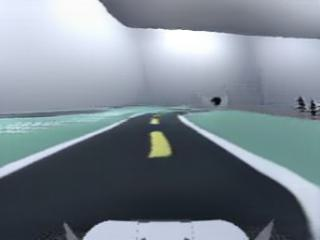
\includegraphics[width=1\textwidth]{experiments/0__.jpg}}
	      \caption{Pseudo-simulated image}\label{fig:psim}
	  \end{subfigure}%
  \hfill
  \begin{subfigure}{.33\linewidth}
	    \centering
	    \scalebox{-1}[1]{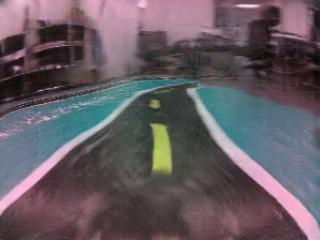
\includegraphics[width=1\textwidth]{experiments/0___.jpg}}
	    \caption{Pseudo-pseudo-real image}\label{fig:ppreal}
	  \end{subfigure} 
  \caption{Using the CycleGan to create a paired dateset}
  \label{fig:examplealigned}
\end{figure}

However, we can visually see that the quality of the translations degrades as more transformation steps are applied. Once obtained the paired dataset of authentic and pseudo images we computed the respective latent space vectors and used t-SNE to visualize them. The results are shown in Figure~\ref{fig:latentpseudoaligned}.

\begin{figure}[h]
  \centering
  \begin{subfigure}{.5\linewidth}
	      \centering
	      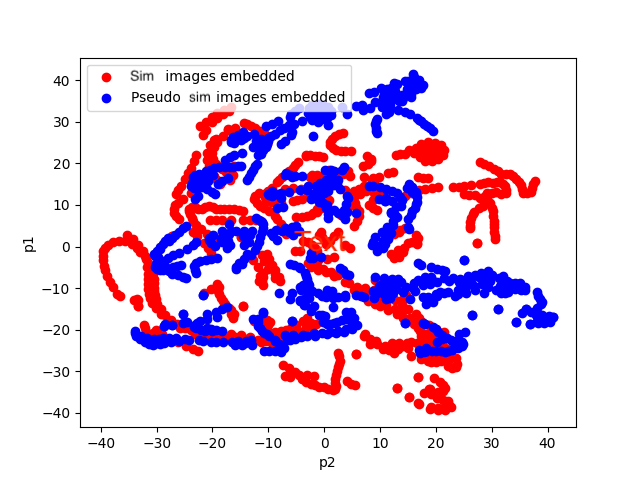
\includegraphics[width=1\textwidth]{experiments/aligned_latentr2s.png}
	      \caption{Paired Simulated (authentic) and pseudo-simulated images. \matteo{check labels}}\label{fig:aligen_latentr2s}
	  \end{subfigure}%
      \hfill
  \begin{subfigure}{.5\linewidth}
	      \centering
	      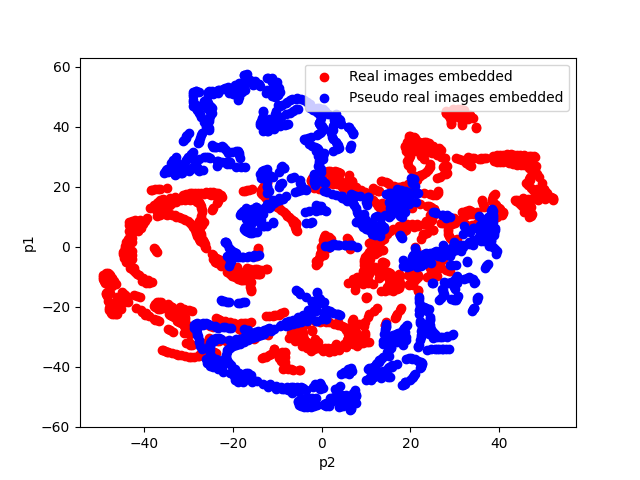
\includegraphics[width=1\textwidth]{experiments/aligned_latents2r.png}
	      \caption{Paired Real (authentic) and pseudo-real images.}\label{fig:aligen_latents2r}
	  \end{subfigure}
  \caption{Latent space visualization for the paired datasets: authentic vs pseudo (i.e., translated) images. (Left) simulated VAE, (right) real VAE.}
  \label{fig:latentpseudoaligned}
\end{figure}

However, the overlap of the embeddings does not seem to increase w.r.t. the unpaired datasets. We further proceeded with a more fine-grained analysis by looking at the single images in the datasets. In particular, considering the paired datasets, we randomly sampled pseudo images and computed their latent space representation. Then, we computed the Euclidean distance between such representation and all latent space representations in the authentic paired dataset and took the corresponding image whose latent space is the closest. Examples of such images are in Figure~\ref{fig:simdistance} for the simulated environment and in Figure~\ref{fig:realdistance}.

%Unfortunately, the results do not change enough from the previous one as shown in Figure \ref{fig:latentpseudoaligned}. Given that the t-SNEe dimensionality reduction may be a cause of our problem, a further investigation is made by checking what are the closest images between the real set and pseudo real set and similarly for the simulated set in the latent space. The distance measure used is the Euclidean distance and by looking at them there is some problem, in fact there are perfect matches as well as wrong matches as shown in Figures \ref{fig:simdistance} and \ref{fig:realdistance}. This may be the cause of our agent not being able to drive when transferred into another domain, the encoder is not robust enough to compensate little image distortion.

\begin{figure}[h]
  \centering
  \begin{subfigure}{.24\linewidth}
	      \centering
	      \scalebox{-1}[1]{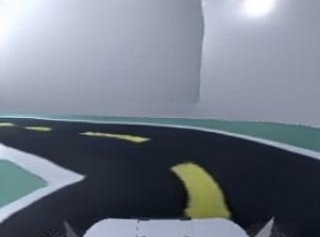
\includegraphics[width=1\textwidth]{experiments/badsimdist1.jpg}}
	      \caption{Pseudo simulated (Bad)}\label{fig:badsimdist1}
	  \end{subfigure}%
  \hfill
  \begin{subfigure}{.24\linewidth}
	    \centering
	    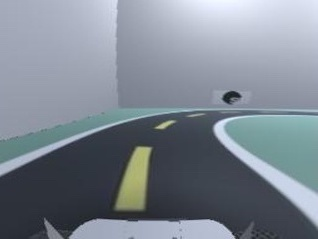
\includegraphics[width=1\textwidth]{experiments/badsimdist2.jpg}
	    \caption{Closest simulated (Bad)}\label{fig:badsimdist2}
	  \end{subfigure}%
  \hfill
  \begin{subfigure}{.24\linewidth}
	      \centering
	      \scalebox{-1}[1]{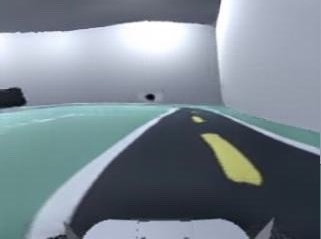
\includegraphics[width=1\textwidth]{experiments/goodsimdist1.jpg}}
	      \caption{Pseudo simulated (Good)}\label{fig:goodsimdist1}
	  \end{subfigure}%
  \hfill
  \begin{subfigure}{.24\linewidth}
	    \centering
	    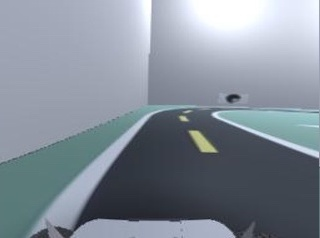
\includegraphics[width=1\textwidth]{experiments/goodsimdist2.jpg}
	    \caption{Closest simulated (Good)}\label{fig:goodsimdist2}
	\end{subfigure}
	  \caption{Figure~\ref{fig:badsimdist1} and Figure~\ref{fig:goodsimdist1} show two pseudo-simulated images. Respectively, Figure~\ref{fig:badsimdist2} and Figure~\ref{fig:goodsimdist2} are the closest match in the simulated set according to the Euclidean distance in the latent space of the simulated VAE.}
	  \label{fig:simdistance}
\end{figure}


\begin{figure}[h]
  \centering
  \begin{subfigure}{.24\linewidth}
	      \centering
	      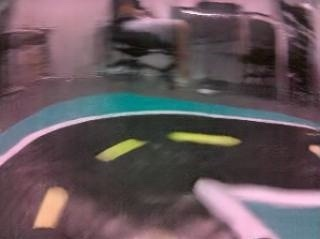
\includegraphics[width=1\textwidth]{experiments/badrealreal1.jpg}
	      \caption{Pseudo real (Bad)}\label{fig:badrealdist1}
	  \end{subfigure}%
  \hfill
  \begin{subfigure}{.24\linewidth}
	    \centering
	    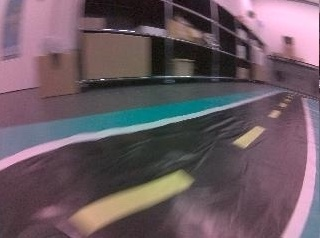
\includegraphics[width=1\textwidth]{experiments/badrealreal2.jpg}
	    \caption{Closest real (Bad)}\label{fig:badrealdist2}
	  \end{subfigure}%
  \hfill
  \begin{subfigure}{.24\linewidth}
	      \centering
	      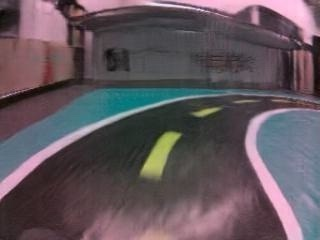
\includegraphics[width=1\textwidth]{experiments/goodrealdist1.jpg}
	      \caption{Pseudo real (Good)}\label{fig:goodrealdist1}
	  \end{subfigure}%
  \hfill
  \begin{subfigure}{.24\linewidth}
	    \centering
	    \includegraphics[width=1\textwidth]{experiments/goodrealdist2.jpg}
	    \caption{Closest real (Good)}\label{fig:goodrealdist2}
	\end{subfigure}
	  \caption{Figure~\ref{fig:badrealdist1} and Figure~\ref{fig:goodrealdist1} show two pseudo-real images. Respectively, Figure~\ref{fig:badrealdist2} and Figure~\ref{fig:goodrealdist2}, show the closest match in the real set according to the Euclidean distance in the latent space of the real VAE.}
	  \label{fig:realdistance}
\end{figure}

We can see from the images that in some cases the closest image in the latent space is actually similar to the authentic counterpart (see Good examples). On the other hand, there are also examples in critical parts of the track (see Figure~\ref{fig:badsimdist1} and Figure~\ref{fig:badrealdist1}), in which the closest authentic image in the latent space does not actually represent what is in the pseudo counterpart. As a consequence, transferring a trained agent from one domain into the other by using image-to-image translation seems challenging, as the VAE that represents the state for the trained policy does not seem to be robust w.r.t. the translations.

Finally, we analyzed the offline predictions of the agent we trained in the real world and compute the error between the prediction made by the agent when given the authentic real image and the prediction made when given the pseudo-real image. Specifically, we selected a set of 100 contiguous images from the real dataset and computed the corresponding paired translation, i.e. from real to simulated and from simulated to real \matteo{images of which sector of the track? Moreover, 100 images correspond to 5 seconds of simulation}. Then, we computed the prediction, i.e. the steering angle, of the trained agent when given each of the two images and plotted the results in Figure~\ref{fig:path_rec}. From the plot we can see that, most of the time, the predictions are aligned. The average prediction error is 0.205 with a standard deviation of 0.183. However, small prediction errors can accumulate over time leading the car in sectors of the track where it is not able to recover.

%As a final test, we are interested in studying what would be the actions undertaken by the agent on a set of aligned pictures. In particular, we selected a small set of 100 contiguous real pictures of the track and created its \textit{aligned} pseudo real version. We then checked what would be the action of the real agent. As shown in Figure \ref{fig:path_rec}, the results are interesting since most of the times the agent takes the same action on both images, however even a tiny difference can lead the car out of track from which often it is not able to recover. The mean error on the predicted action resulted to be 0.20 
%TODO INSERIRE STD E BREVE CONCLUSIONE DELLA SEZIONE 

\begin{figure}[h]
  \begin{center}
	    \includegraphics[width=0.60\textwidth]{experiments/path_rec.png}
	  \end{center}
  \caption{Trained agent predictions when given authentic real image and pseudo-real image.}
  \label{fig:path_rec}
\end{figure}

%\begin{figure}[h]
%  \begin{center}
	%    \includegraphics[width=0.60\textwidth]{experiments/path_rec.png}
	%  \end{center}
%  \caption{Real agent's actions on an aligned dataset}
%  \label{fig:path_rec}
%\end{figure}

%\begin{figure}[h]
%  \centering
%  \begin{subfigure}{.24\linewidth}
	%      \centering
	%      \scalebox{-1}[1]{\includegraphics[width=1\textwidth]{experiments/badsimdist1.jpg}}
	%      \caption{Pseudo simulated}\label{fig:badsimdist1}
	%  \end{subfigure}%
%  \hfill
%  \begin{subfigure}{.24\linewidth}
	%    \centering
	%    \includegraphics[width=1\textwidth]{experiments/badsimdist2.jpg}
	%    \caption{Closest simulated}\label{fig:badsimdist2}
	%  \end{subfigure}%
%  \hfill
%  \begin{subfigure}{.24\linewidth}
	%      \centering
	%      \scalebox{-1}[1]{\includegraphics[width=1\textwidth]{experiments/goodsimdist1.jpg}}
	%      \caption{Pseudo simulated}\label{fig:goodsimdist1}
	%  \end{subfigure}%
%  \hfill
%  \begin{subfigure}{.24\linewidth}
%    \centering
%    \includegraphics[width=1\textwidth]{experiments/goodsimdist2.jpg}
%    \caption{Closest simulated}\label{fig:goodsimdist2}
%\end{subfigure}
%  \caption{Figures \ref{fig:badsimdist1} and \ref{fig:goodsimdist1} show two pseudo simulated images and Figures \ref{fig:badsimdist2} and \ref{fig:goodsimdist2} respectively the closest match in the simulated set measured with the Euclidean Distance.}
%  \label{fig:simdistance}
%\end{figure}

%\begin{figure}[h]
%  \centering
%  \begin{subfigure}{.24\linewidth}
	%      \centering
	%      \includegraphics[width=1\textwidth]{experiments/badrealreal1.jpg}
	%      \caption{Pseudo real}\label{fig:badrealdist1}
	%  \end{subfigure}%
%  \hfill
%  \begin{subfigure}{.24\linewidth}
	%    \centering
	%    \includegraphics[width=1\textwidth]{experiments/badrealreal2.jpg}
	%    \caption{Closest real}\label{fig:badrealdist2}
	%  \end{subfigure}%
%  \hfill
%  \begin{subfigure}{.24\linewidth}
	%      \centering
	%      \includegraphics[width=1\textwidth]{experiments/goodrealdist1.jpg}
	%      \caption{Pseudo real}\label{fig:goodrealdist1}
	%  \end{subfigure}%
%  \hfill
%  \begin{subfigure}{.24\linewidth}
	%    \centering
	%    \includegraphics[width=1\textwidth]{experiments/goodrealdist2.jpg}
	%    \caption{Closest real}\label{fig:goodrealdist2}
	%\end{subfigure}
	%  \caption{Figures \ref{fig:badrealdist1} and \ref{fig:goodrealdist1} show two pseudo real images and Figures \ref{fig:badrealdist2} and \ref{fig:goodrealdist2} respectively the closest match in the real set measured with the Euclidean Distance.}
	%  \label{fig:realdistance}
	%\end{figure}


%Unfortunately, the results do not change enough from the previous one as shown in Figure \ref{fig:latentpseudoaligned}. Given that the t-SNEe dimensionality reduction may be a cause of our problem, a further investigation is made by checking what are the closest images between the real set and pseudo real set and similarly for the simulated set in the latent space. The distance measure used is the Euclidean distance and by looking at them there is some problem, in fact there are perfect matches as well as wrong matches as shown in Figures \ref{fig:simdistance} and \ref{fig:realdistance}. This may be the cause of our agent not being able to drive when transferred into another domain, the encoder is not robust enough to compensate little image distortion.


%Hence, the real test set is transformed through the CycleGAN and then forwarded through the real VAE chosen and similarly for the simulated test set. Given that 64 dimension cannot be visualized, a further dimensionality reduction is applied with t-SNE down to two dimension, as shown in Figure \ref{fig:latentpseudo}.
%
%\begin{figure}[h]
%  \centering
%  \begin{subfigure}{.5\linewidth}
%      \centering
%      \includegraphics[width=1\textwidth]{experiments/latentr2s.png}
%      \caption{Simulated and pseudo simulated images}\label{fig:latentr2s}
%  \end{subfigure}%
%      \hfill
%  \begin{subfigure}{.5\linewidth}
%      \centering
%      \includegraphics[width=1\textwidth]{experiments/latents2r.png}
%      \caption{Real and pseudo real images}\label{fig:latents2r}
%  \end{subfigure}
%  \caption{Images embedded into the latent space with respectively the simulated and the real VAE.}
%  \label{fig:latentpseudo}
%\end{figure}
%Since the datasets are not aligned we do not except a perfect overlap, instead, the encoder should be able to at least embed similar images in the same region of the space. However, the latent space shows that is not always the case, some regions does overlap but not all off them in both real and simulated dataset. This could lead the trained agent not to respond consistently in similar situations. A further attempt is made by aligning the set of data used through the CycleGAN. Once the CycleGAN has been used to transform simulated images into pseudo real images, it can be used again to bring them back to pseudo simulated images, resulting in aligned sets. However, notice that the distortion, barely visible before, increases as shown in Figure \ref{fig:examplealigned}.
%
%\begin{figure}[h]
%  \centering
%  \begin{subfigure}{.33\linewidth}
%      \centering
%      \includegraphics[width=1\textwidth]{experiments/0_.jpg}
%      \caption{Real image}\label{fig:real}
%  \end{subfigure}%
%      \hfill
%  \begin{subfigure}{.33\linewidth}
%      \centering
%      \scalebox{-1}[1]{\includegraphics[width=1\textwidth]{experiments/0__.jpg}}
%      \caption{Pseudo simulated image}\label{fig:psim}
%  \end{subfigure}%
%  \hfill
%  \begin{subfigure}{.33\linewidth}
%    \centering
%    \scalebox{-1}[1]{\includegraphics[width=1\textwidth]{experiments/0___.jpg}}
%    \caption{Pseudo pseudo real}\label{fig:ppreal}
%  \end{subfigure} 
%  \caption{Example of using the CycleGan to create an aligned dateset}
%  \label{fig:examplealigned}
%\end{figure}
%
%\begin{figure}[h]
%  \centering
%  \begin{subfigure}{.5\linewidth}
%      \centering
%      \includegraphics[width=1\textwidth]{experiments/aligned_latentr2s.png}
%      \caption{Aligned simulated and pseudo sim images}\label{fig:aligen_latentr2s}
%  \end{subfigure}%
%      \hfill
%  \begin{subfigure}{.5\linewidth}
%      \centering
%      \includegraphics[width=1\textwidth]{experiments/aligned_latents2r.png}
%      \caption{Aligned real and pseudo real images}\label{fig:aligen_latents2r}
%  \end{subfigure}
%  \caption{Aligned images embedded into the latent space with respectively the simulated and the real VAE.}
%  \label{fig:latentpseudoaligned}
%\end{figure}
%
%Unfortunately, the results do not change enough from the previous one as shown in Figure \ref{fig:latentpseudoaligned}. Given that the t-SNEe dimensionality reduction may be a cause of our problem, a further investigation is made by checking what are the closest images between the real set and pseudo real set and similarly for the simulated set in the latent space. The distance measure used is the Euclidean distance and by looking at them there is some problem, in fact there are perfect matches as well as wrong matches as shown in Figures \ref{fig:simdistance} and \ref{fig:realdistance}. This may be the cause of our agent not being able to drive when transferred into another domain, the encoder is not robust enough to compensate little image distortion.
%
%As a final test, we are interested in studying what would be the actions undertaken by the agent on a set of aligned pictures. In particular, we selected a small set of 100 contiguous real pictures of the track and created its \textit{aligned} pseudo real version. We then checked what would be the action of the real agent. As shown in Figure \ref{fig:path_rec}, the results are interesting since most of the times the agent takes the same action on both images, however even a tiny difference can lead the car out of track from which often it is not able to recover. The mean error on the predicted action resulted to be 0.20 
%TODO INSERIRE STD E BREVE CONCLUSIONE DELLA SEZIONE 
%
%\begin{figure}[h]
%  \begin{center}
%    \includegraphics[width=0.60\textwidth]{experiments/path_rec.png}
%  \end{center}
%  \caption{Real agent's actions on an aligned dataset}
%  \label{fig:path_rec}
%\end{figure}
%
%\begin{figure}[h]
%  \centering
%  \begin{subfigure}{.24\linewidth}
%      \centering
%      \scalebox{-1}[1]{\includegraphics[width=1\textwidth]{experiments/badsimdist1.jpg}}
%      \caption{Pseudo simulated}\label{fig:badsimdist1}
%  \end{subfigure}%
%  \hfill
%  \begin{subfigure}{.24\linewidth}
%    \centering
%    \includegraphics[width=1\textwidth]{experiments/badsimdist2.jpg}
%    \caption{Closest simulated}\label{fig:badsimdist2}
%  \end{subfigure}%
%  \hfill
%  \begin{subfigure}{.24\linewidth}
%      \centering
%      \scalebox{-1}[1]{\includegraphics[width=1\textwidth]{experiments/goodsimdist1.jpg}}
%      \caption{Pseudo simulated}\label{fig:goodsimdist1}
%  \end{subfigure}%
%  \hfill
%  \begin{subfigure}{.24\linewidth}
%    \centering
%    \includegraphics[width=1\textwidth]{experiments/goodsimdist2.jpg}
%    \caption{Closest simulated}\label{fig:goodsimdist2}
%\end{subfigure}
%  \caption{Figures \ref{fig:badsimdist1} and \ref{fig:goodsimdist1} show two pseudo simulated images and Figures \ref{fig:badsimdist2} and \ref{fig:goodsimdist2} respectively the closest match in the simulated set measured with the Euclidean Distance.}
%  \label{fig:simdistance}
%\end{figure}
%
%\begin{figure}[h]
%  \centering
%  \begin{subfigure}{.24\linewidth}
%      \centering
%      \includegraphics[width=1\textwidth]{experiments/badrealreal1.jpg}
%      \caption{Pseudo real}\label{fig:badrealdist1}
%  \end{subfigure}%
%  \hfill
%  \begin{subfigure}{.24\linewidth}
%    \centering
%    \includegraphics[width=1\textwidth]{experiments/badrealreal2.jpg}
%    \caption{Closest real}\label{fig:badrealdist2}
%  \end{subfigure}%
%  \hfill
%  \begin{subfigure}{.24\linewidth}
%      \centering
%      \includegraphics[width=1\textwidth]{experiments/goodrealdist1.jpg}
%      \caption{Pseudo real}\label{fig:goodrealdist1}
%  \end{subfigure}%
%  \hfill
%  \begin{subfigure}{.24\linewidth}
%    \centering
%    \includegraphics[width=1\textwidth]{experiments/goodrealdist2.jpg}
%    \caption{Closest real}\label{fig:goodrealdist2}
%\end{subfigure}
%  \caption{Figures \ref{fig:badrealdist1} and \ref{fig:goodrealdist1} show two pseudo real images and Figures \ref{fig:badrealdist2} and \ref{fig:goodrealdist2} respectively the closest match in the real set measured with the Euclidean Distance.}
%  \label{fig:realdistance}
%\end{figure}




\chapter{Future work and conclusion}

Another reward function was initally tested trying to improve the total time an agent takes to complete a lap:
\begin{equation}
  \label{eq:testreward}
  r_t = - 0.1 + throttle\_reward + cte\_penalty + \left\{\begin{matrix}
    if done & crash\_error \\ 
    else & 0  
    \end{matrix}\right.
\end{equation}
The idea behind this function is that any step gives a negative reward and thus the agent must finish a lap in the smallest number of step to maximize the total episode reward. Minimizing the number steps means also finding the shortest way and consequently reducing the total time spent for a lap. Unfortunately, this approach did not let the agent learn to drive decently, at least in reasonable time.

\appendix %optional, use only if you have an appendix

\chapter{Some retarded material}
Lara
\section{It's over\dots}
Ciaooo mbareeeeee

\backmatter

\chapter{Glossary} %optional

%\bibliographystyle{alpha}
%\bibliographystyle{dcu}
\bibliographystyle{plainnat}
\bibliography{biblio}

%\cleardoublepage
%\theindex %optional, use only if you have an index, must use
	  %\makeindex in the preamble

\end{document}